% \documentclass[draft]{report}

\RequirePackage{luatex85}% TeXLive 2017 fix for \geometry
\documentclass{kdp}
\usepackage{geometry}

% \usepackage{algorithm}% http://ctan.org/pkg/algorithms
\usepackage{algpseudocode}% http://ctan.org/pkg/algorithmicx
% \usepackage{algorithm}% http://ctan.org/pkg/algorithms
% \usepackage{algpseudocode}
\usepackage{tlatex}
\usepackage{listings}
\usepackage{xcolor}
\usepackage{comment}
\usepackage{fancyhdr}
\usepackage{amssymb}
\usepackage{inputenc}
\usepackage{svg}
\usepackage{framed}
\usepackage{graphicx}
\usepackage{tikz}
\usetikzlibrary{automata, positioning, arrows}

% \usepackage{hyperref}
% \hypersetup{
%     colorlinks,
%     citecolor=black,
%     filecolor=black,
%     linkcolor=black,
%     urlcolor=black
% }

% !TeX spellcheck = en_GB 

% Configure fancyhdr
\pagestyle{fancy}
\fancyhf{} % Clear default header and footer

% Header settings
\fancyhead[L]{\nouppercase{\leftmark}} % Chapter number and title on the left
% \fancyhead[C]{Center Header}    % Centered header
\fancyhead[R]{\thepage}     % Right-aligned header

% Footer settings
% \fancyfoot[L]{Left Footer}      % Left-aligned footer
% \fancyfoot[C]{Page \thepage}    % Centered footer with page number
% \fancyfoot[R]{Right Footer}     % Right-aligned footer

% java -cp /home/richard/dev/tla2tex/tla2tools.jar  tla2tex.TeX  book.tex 

\lstset { %
    language=C++,
    backgroundcolor=\color{black!5}, % set backgroundcolor
    basicstyle=\footnotesize,% basic font setting
}

\title{\textit{Correct by Design} with TLA+ \\ Early Preview}

% \maketitle



\author{Richard Tang}
\date{\today}
\begin{document}
\maketitle

% \vspace{1cm} % Adjust spacing as needed
% \begin{center}
% \textbf{First Draft}
% \end{center}

\section*{Acknowledgement}

A big thanks to Anthony Giardina for reviewing the content of this book.

\tableofcontents

\part{Introduction}

\chapter{Motivation}

\section{Catching Problems Early}

Years ago, I worked on a propietary low power processor in an embedded system.
The processor ran microcode featuring a custom instruction set. To enter a low
power state, a set of (possibly hundreds) instructions were executed. These
instructions progressively puts the system in lower power state. For example:
turn off IP A, then turn off IP B, then turn off the power island to the IPs. To
save cost and power, the low power processor had very limited debuggability
support.\newline

An experienced reader may start to notice some redflags.\newline

If the microcode attempts to access the memory interface when the power island
has been shut off, processor would hang. Since the power island has been shut
off, the physical hardware debug port is also unavailable, leaving the developer
with \textit{no way} of live debugging related problem. At this point the
developer needs to siphon through (possibly hundreds) of instructions to catch
invariant violation \textit{manually}.\newline

As one can imagine, maintaining the microcode was very expensive. Fortunately,
the propietary low power processor only had a handful of instructions, I created
an emulator for this propietary processor to verify the microcode prior to
deploying it on target. The emulator models the processor states as a state
graph, with executed instruction transitions the state machine to the next
state. At every state all the invariants are evaluated to ensure none have been
violated. Some of the invariants included:
\begin{itemize}
    \item Accessing memory interface after power off leads to a hang
    \item Accessing certain register in certain chip revision leads to a hang 
    \item Verify IPs are shut off in the allowed order
\end{itemize}

The verification algorithm was implemented using a \textit{depth-first search}
algorithm, providing 100\% microcode coverage before deploy on target.\newline

To generalize, we can model arbitrary system as a set of states with a
collection of invariant that must be upheld at all times. The complexity of the
such arbitrarily system generally grows quadratically as the number of states
grow linearly (eg. in a N state system, adding state N+1 may introduce N
transitions into the new state). There are many engineering problems that
exhibit a large number of states, such as lockless or waitfree data structure,
distributed algorithms, OS scheduler, and more. As the number of states grow, 
the problem becomes more mentally taxing for designer to reason about.\newline

\textit{How does a designer reason about the correctness of a proposed
solution?}

\section{The Generalized Problem}

Fast forward to now: I stumbled across TLA+, a formalized solution of what I was
looking for.\newline

The Turing Award winner Leslie Lamport invented the TLA+ 1999, but TLA+ didn't
appear to have caught on until the 2010's. My opinion is TLA+ was invented ahead
of its time, and the problem complexity finally caught up in the past decade or
so, to allow TLA+ to demonstrate its strength.\newline

We are at a point in the technology curve where vertical scaling is no longer
practical, with CPU speed plateau'd in the past decade or so. The industry is
exploring horizontal scaling solution, such as hardware vendor focusing adding
more CPU cores, or software vendors buying many low end hardware instead of a
few high end hardware. This shifts the technology complexity from vertical to
horizontal, demanding solution to maximize concurrent resource utilization.
There is one slight problem though:\newline

\textit{Humans are not good at reasoning about things happening
concurrently.}\newline

Our cognitive system is optimized for sequential reasoning. Enumerating all
scenarios in one's mind to ensure an arbitrary design accommodates all the
corner cases is challenging.\newline

Consider a low power processor execution hundreds of instruction, how does the 
designer ensure the invariants are upheld after every instruction?\newline

Consider a distributed system. The system is a cluster of independently
operating entities and need to somehow collectively offer the correct system
behaviour, while any one of the machines may receive instructions out of order,
crash, recover, etc. \newline

Consider a single producer multiple consumer lockless queue. The consumers may 
reserve an index in the queue in certain order, but may release them in different order. 
What if one reader is really slow, and another reader is super fast and possibly 
lapse the slow reader? \newline

Consider an OS scheduler with locks. Assume all the processes have the same
priority. Can a process starve the other processes by repeatedly acquire and
release the lock? How do we ensure scheduling is fair?\newline

% One \textit{anti-solution} is to assert that these are easy problem for designer
% with the right experience and skill set. While this may be true, it also isn't
% very scalable. It is likely to your organization's 

The \textit{anti-pattern} is to keep bandaiding the design until user stops
filing bug reports. This is never ideal. Per Murphy's law, anything that can go
wrong \textit{will go wrong}, and a hard to reproduce bug will come in at the
most inconvinient time. How do we make sure the solution is \textit{correct by
design}? To solve this problem, we must rely on tools to do the reasoning
\textit{for us}.

\section{What is TLA+?}

TLA+ is a \textit{system specification language}, with the intent to describe
the system with implementation details removed. TLA+ allows designer to describe
the system as a sequence of states. The designer can expresses transition
condition from one state to another, describe invariants that must hold true in
every state and liveness properties that the overall system should converge to.
The key innovation of TLA+ is once the system is modeled as a finite state
machine, the states can be \textit{exhaustively} explored (via
breath-first-search) to ensure certain properties are held through out the
entire state space (either per state or a sequence of states).\newline

\section{About This Book}

To my surprise, there is not as much material on TLA+ as I assumed for such
critical tools in a designer's toolbox. This book was initially a set of notes I
took while learning TLA+. I decided to formalize these notes into this short
book, which I hope the readers will find helpful in their TLA+ journey.\newline

The intent for the book is to teach reader how to write TLA+ spec for their
design to provide confidence in \textit{design correctness}. This book is
targeted to software designer, hardware designer, system architect, and in
general anyone who is interested in designing correct system.\newline 

To get the most out of the book, reader should have general computing science
knowledge. Reader doesn't need to be expert at a particular language to
understand this book; TLA+ is effectively its own language. This book is example
driven and will go through designs such as lockless queue, simple task
scheduler, consensus algorithm, etc. Reader will likely enjoy a deeper insight
if she has some familiarity with these topics.

\section{How to Use This Book}

This book was designed to be used as a reference, providing examples and
references using TLA+.\newline

Examples are split into two categories: A set of examples written using TLA+,
and another set of examples written using PlusCal (the C-like syntax that
transpiles down to TLA+). I believe they are useful for different use cases.
The differences will be highlighted in their respective sections. All examples
will follow a similar layout, covering the requirements, design, spec, and 
safety properties.\newline

All examples in this book will be presented using TLA+ \textit{mathemetical
notation}. Converting between Mathmetical and ASCII notation is assumed
straightforward due to the one-to-one mapping. Readers are encouraged to consult
Table 8 in \cite{ss} as needed.\newline

The last part of the book provides that language reference and some focused
topic. Reader can use the last part of the book as a general reference. 



\chapter{TLA+ Primer}

\section{Purpose}

The key insight to TLA+ is modeling a system as a state machine. A simple
digital clock can be represented by two variables, hour and minute and the
number of possible states in a digital clock is $24 * 60 = 1440$. For example,
a clock in state 10:00 will transition to state 10:01. Asssume an arbitrarily
system described by N variables, each variable having K possible values such
arbitrary system can have up to $N^K$ state.\newline

For every specification, designer can specify \textit{safety} proerty (or
invariants) that must be true in \textit{every} states. For example, in any
state of the digital clock hour \textit{must} be between 0 to 23, or formally
described as $hour \in 0..23$. Similarly, minute must have value between 0 to
59, or $minute \in 0..59$. Examples invariants of a system include: Only one
thread has exclusive access to a critical region, all variables in the system
are within allowable value, resource allocation manager never allocates more
than available resources.\newline

Designer can also specify \textit{liveness} property. These are properties to be
satisfied by a \textit{sequence of state}. One liveness property for the digital
clock could be when the clock is 10:00, it will eventually become 11:00 (10:00
\textit{leads} to 11:00). Example liveness property include: a distributed
system eventually converges, the scheduler eventually schedules every tasks in
the task queue, the resource allocation manager fairly allocates resources.
\newline

A TLA+ Spec can be checked by TLC, the model checker. TLC uses
\textit{breath-first search} algorithm to explore \textit{all} states in the
state machine and ensure safety and liveness properties are upheld.\newline

A TLA+ Spec describes the system using \textit{temporal logic}. The syntax may 
appear unfamiliar if one hasn't seen it before, but like any other programming 
language an initiated reader should become familiarized quickly.

\section{Design}

In this example, we will specify a \textit{digital clock}. The digital clock has
a few simple requirements:
\begin{itemize}
    \item Two variables to represent state: hour and minute
    \item The clock increment one minute at a time
    \item Hour is between 0 to 23, inclusive
    \item Minute is between 0 to 59, inclusive
    \item Clock wraps around at midnight (ie. 23:59 transitions to 00:00)
\end{itemize}

\section{Spec}

The \textit{Init} state of such system can be described as: \newline
\begin{tla}
    vars == <<hour, minute>>
    Init ==
        /\ hour = 0
        /\ minute = 0
\end{tla}
\begin{tlatex}
\@x{\@s{16.4} Init \.{\defeq}}%
\@x{\@s{32.8} \.{\land} hour \.{=} 0}%
\@x{\@s{32.8} \.{\land} minute \.{=} 0}%
\end{tlatex}
 \newline

$\defeq$ is the \textit{defines equal} symbol and $\land$ is the \textit{logical
and} symbol. The above TLA+ syntax can be read as \textit{Init} state is defined
as both hour and minute are 0.\newline

The spec also always include a \textit{Next} definition, an \textit{action
formula} describing how the system transition from one state to another. Action
formula contains \textit{primed} variables what happens to the variable in its
next state. The \textit{Next} action for the digital clock can be defined
as:\newline

\begin{tla}
    NextHour ==
        /\ minute = 59 
        /\ hour' = (hour + 1) % 24
        /\ minute' = 0
    NextMinute == 
        /\ minute # 59
        /\ hour' = hour 
        /\ minute' = minute + 1 
    Next ==
        \/ NextMinute
        \/ NextHour
\end{tla}
\begin{tlatex}
\@x{\@s{16.4} NextHour \.{\defeq}}%
\@x{\@s{32.8} \.{\land} minute \.{=} 59}%
\@x{\@s{32.8} \.{\land} hour \.{'} \.{=} ( hour \.{+} 1 ) \.{\%} 24}%
\@x{\@s{32.8} \.{\land} minute \.{'} \.{=} 0}%
\@x{\@s{16.4} NextMinute \.{\defeq}}%
\@x{\@s{32.8} \.{\land} minute \.{\neq} 59}%
\@x{\@s{32.8} \.{\land} hour \.{'} \.{=} hour}%
\@x{\@s{32.8} \.{\land} minute \.{'} \.{=} minute \.{+} 1}%
\@x{\@s{16.4} Next \.{\defeq}}%
\@x{\@s{32.8} \.{\lor} NextMinute}%
\@x{\@s{32.8} \.{\lor} NextHour}%
\end{tlatex}
 \newline

Here's a breakdown of what the spec does:
\begin{itemize}
    \item \textit{Next} can take either \textit{NextHour} or \textit{NextMinute}
    \item \textit{Next} takes \textit{NextMinute} when \textit{minute} is not
    59. \textit{NextMinute} doesn't update \textit{Hour} and increments \textit{Minute}.
    \item \textit{Next} takes \textit{NextHour} when \textit{minute} is 59.
    \textit{NextHour} increments \textit{hour} modulus 24 and sets \textit{minute} to 0.
\end{itemize}

Note that the formulas are \textit{state descriptions}, not \textit{assignment}.
\textit{minute = 59} describes the state transition takes when minute
\textit{equals} 59. Since this is an equality description, \textit{minute = 59}
and \textit{59 = minute} are equivalent in TLA+.\newline

Finally, the Spec itself is formally defined as:\newline
\begin{tla}
    Spec ==
        /\ Init
        /\ [][Next]_vars
\end{tla}
\begin{tlatex}
\@x{\@s{16.4} vars\@s{0.63} \.{\defeq} {\langle} hour ,\, minute {\rangle}}%
\@x{\@s{16.4} Spec \.{\defeq}}%
\@x{\@s{32.8} \.{\land} Init}%
\@x{\@s{32.8} \.{\land} {\Box} [ Next ]_{ vars}}%
\end{tlatex}
\newline

Note this forms the basis for \textbf{all} TLA+ Spec. Every example in this book
will include a Spec definition similar to this. \newline

$\Box[Next]_{vars}$ deserves some special attention:
\begin{itemize}
    \item $vars$ is defined earlier to be \textit{all} variables in the spec, in
    this case hour and minute. Combination of these variables at different
    values constitute the states of the system (eg. 23:59 and 00:00 are differente
    states in the system).
    \item $\Box[Next]_{vars}$ is a box-action formula, where \textit{Next} is an
    action and \textit{vars} is a state function.
    \item $\Box$ operator asserts the formula is always true for every step in the behaviour.
    \item And steps in the behaviour is defined as $[Next]_{vars}$, where $Next$
    describe the action and $vars$ capturing all variables representing the state.
\end{itemize}

This can be roughly translate to: the system is valid for for every step
\textit{Next} can take, forming the basis of the Spec.

\section{Safety}

Safety property describes invariant that must hold true in \textit{every} state
of system. A common invariant is \textit{type safety} checks. In a digital
clock, hour can only be in value between 0 to 23, and minute can only be value
of 0 to 59:\newline

\begin{tla}
    Type_OK == 
        /\ hour \in 0..23
        /\ minute \in 0..59
\end{tla}
\begin{tlatex}
\@x{\@s{16.4} Type\_OK \.{\defeq}}%
\@x{\@s{32.8} \.{\land} hour \.{\in} 0 \.{\dotdot} 23}%
\@x{\@s{32.8} \.{\land} minute \.{\in} 0 \.{\dotdot} 59}%
\end{tlatex}
\newline

When hour or minute falls outside of the specified range, the model checker 
reports failure.

\section{Liveness}

Liveness property verifies certain behavioural across a sequence of state. One
liveness property is to confirm the clock wraps around at midnight, a property
that can only be verified after checking at least two states: \newline

\begin{tla}
    Liveness ==
        /\ hour = 23 /\ minute = 59 ~> hour = 0 /\ minute = 0
\end{tla}
\begin{tlatex}
\@x{\@s{16.4} Liveness \.{\defeq}}%
 \@x{\@s{32.8} \.{\land} hour \.{=} 23 \.{\land} minute \.{=} 59 \.{\leadsto}
 hour \.{=} 0 \.{\land} minute \.{=} 0}%
\end{tlatex}
\newline

$\leadsto$ is the \textit{leads to} operator, suggesting something is eventually
true. TLA+ provides a set of operators to describe liveness property.\newline 

To verify liveness, we need to modify the spec slightly to enable
\textit{fairness} to prevent \textit{stuttering}. In plain terms, fairness
ensure a state always transition to \textit{some other state}. Without fairness
the spec is allowed to \textit{stutter}, or \textit{not transition} to any state. 
This by definition fails liveness property check as the model checker is
unable to verify the behaviour across a sequence of states. To get a more 
comprehensive description of fairness, refer to the last part of the
book.\newline

\begin{tla}
    Spec ==
        /\ Init
        /\ [][Next]_vars
        /\ WF_vars(Next)
\end{tla}
\begin{tlatex}
\@x{\@s{16.4} Spec \.{\defeq}}%
\@x{\@s{32.8} \.{\land} Init}%
\@x{\@s{32.8} \.{\land} {\Box} [ Next ]_{ vars}}%
\@x{\@s{32.8} \.{\land} {\WF}_{ vars} ( Next )}%
\end{tlatex}
\newline

$WF_{vars}(Next)$ is the fairness qualifier.

% TODO: insert reference here to specifying systems 8.1 

\section{Model Checker}

A TLA+ spec can be verified using model checker. The model checker runs the spec
and verifies all specified safety and liveness properties are fulfilled. The
model checker is a library written in Java, and can be invoked from command
line. For instruction on installing the model checker and related tools, please
see \cite{toolbox}.\newline

After installing the model checker, we need two things to verify the spec:
\begin{itemize}
    \item clock.tla: spec 
    \item clock.cfg: config file
\end{itemize}

For reference, clock.tla is listed below:\newline

\begin{tla}
--------------------------- MODULE clock ----------------------------
EXTENDS Naturals
VARIABLES hour, minute
vars == <<hour, minute>>
Type_OK == 
    /\ hour \in 0..23
    /\ minute \in 0..59
Liveness ==
    /\ hour = 23 /\ minute = 59 ~> hour = 0 /\ minute = 0
Init ==
    /\ hour = 0
    /\ minute = 0
NextMinute ==
    /\ minute = 59 
    /\ hour' = (hour + 1) % 24
    /\ minute' = 0
NextHour == 
    /\ minute # 59
    /\ hour' = hour 
    /\ minute' = minute + 1 
Next ==
    \/ NextMinute
    \/ NextHour
Spec ==
  /\ Init
  /\ [][Next]_vars
  /\ WF_vars(Next)
=============================================================================
\end{tla}
\begin{tlatex}
\@x{}\moduleLeftDash\@xx{ {\MODULE} clock}\moduleRightDash\@xx{}%
\@x{ {\EXTENDS} Naturals}%
\@x{ {\VARIABLES} hour ,\, minute}%
\@x{ vars \.{\defeq} {\langle} hour ,\, minute {\rangle}}%
\@x{ Type\_OK \.{\defeq}}%
\@x{\@s{16.4} \.{\land} hour \.{\in} 0 \.{\dotdot} 23}%
\@x{\@s{16.4} \.{\land} minute \.{\in} 0 \.{\dotdot} 59}%
\@x{ Liveness \.{\defeq}}%
 \@x{\@s{16.4} \.{\land} hour \.{=} 23 \.{\land} minute \.{=} 59 \.{\leadsto}
 hour \.{=} 0 \.{\land} minute \.{=} 0}%
\@x{ Init \.{\defeq}}%
\@x{\@s{16.4} \.{\land} hour \.{=} 0}%
\@x{\@s{16.4} \.{\land} minute \.{=} 0}%
\@x{ NextMinute \.{\defeq}}%
\@x{\@s{16.4} \.{\land} minute \.{=} 59}%
\@x{\@s{16.4} \.{\land} hour \.{'} \.{=} ( hour \.{+} 1 ) \.{\%} 24}%
\@x{\@s{16.4} \.{\land} minute \.{'} \.{=} 0}%
\@x{ NextHour \.{\defeq}}%
\@x{\@s{16.4} \.{\land} minute \.{\neq} 59}%
\@x{\@s{16.4} \.{\land} hour \.{'} \.{=} hour}%
\@x{\@s{16.4} \.{\land} minute \.{'} \.{=} minute \.{+} 1}%
\@x{ Next \.{\defeq}}%
\@x{\@s{16.4} \.{\lor} NextMinute}%
\@x{\@s{16.4} \.{\lor} NextHour}%
\@x{ Spec \.{\defeq}}%
\@x{\@s{8.2} \.{\land}\@s{0.16} Init}%
\@x{\@s{8.2} \.{\land}\@s{0.16} {\Box} [ Next ]_{ vars}}%
\@x{\@s{8.2} \.{\land}\@s{0.16} {\WF}_{ vars} ( Next )}%
\@x{}\bottombar\@xx{}%
\end{tlatex}

The corresponding clock.cfg is listed below: 
\begin{framed}
% \colorlet{shadecolor}{LavenderBlush2}
\begin{verbatim}
SPECIFICATION Spec
INVARIANTS Type_OK
PROPERTIES Liveness
\end{verbatim}
\end{framed}

After putting both clock.cfg and clock.tla in the same directory, one can now
run the model checker. In this book I'll assume a commandline interface for the
model checker:
\begin{verbatim}
java -cp /usr/local/lib/tla2tools.jar tlc2.TLC clock
...
Model checking completed. No error has been found.
  Estimates of the probability that TLC did not check all reachable states
  because two distinct states had the same fingerprint:
  calculated (optimistic):  val = 7.8E-17
1441 states generated, 1440 distinct states found, 0 states left on queue.
The depth of the complete state graph search is 1440.
\end{verbatim}
The 1440 states in the graph represents total number of minutes in a day.


\part{Examples with TLA+}

TLA+ notation is rooted in temporal logic and doesn't share the usual
programming language \textit{look and feel}. Despite the possibly foreign look,
the core language semantics for TLA+ is reasonably constrained. This allows
anyone with some programming experience to pick up relatively quickly. This
section provides a collection of example TLA+ specification with increasing
complexity, easing the readers into this wonderful tool.

% \chapter{Blinking LED}

Let's start with a trivial specification of a blinking LED. The intent of this example 
is to demonstrate the core functionalities of TLA+ specification language.

TODO: briefly talk about tla+ and model checker here.

\section{Requirement}

The LED is represented by a boolean variable that can be either 0 or 1.\newline

... that's it.

\section{Spec}

The specification language may appear alienating as it is mathematically
motivated based on propositional logic. Despite the (possibly) daunting syntax,
designer only need to be familiar with a handful of key operators to start
realizing value using TLA+. This chapter will attempt to describe the example in
exhaustive detail to reduce the learning curve.

The following describe the core portion of the blinking LED spec. 

\begin{tla}
--------------------------- MODULE blinking ----------------------------
VARIABLES b 
vars == <<b>>
Init ==
    /\ b = 0
On == 
    /\ b = 0
    /\ b' = 1
Off == 
    /\ b = 1
    /\ b' = 0
Next ==
    \/ Off 
    \/ On
Spec ==
    /\ Init
    /\ [][Next]_vars
========
\end{tla}
\begin{tlatex}
\@x{}\moduleLeftDash\@xx{ {\MODULE} blinking}\moduleRightDash\@xx{}%
\@x{ {\VARIABLES} b}%
\@x{ vars \.{\defeq} {\langle} b {\rangle}}%
\@x{ Init\@s{2.02} \.{\defeq}}%
\@x{\@s{16.4} \.{\land} b \.{=} 0}%
\@x{ On \.{\defeq}}%
\@x{\@s{18.15} \.{\land} b \.{=} 0}%
\@x{\@s{18.15} \.{\land} b \.{'} \.{=} 1}%
\@x{ Off \.{\defeq}}%
\@x{\@s{15.91} \.{\land} b \.{=} 1}%
\@x{\@s{15.91} \.{\land} b \.{'} \.{=} 0}%
\@x{ Next \.{\defeq}}%
\@x{\@s{16.4} \.{\lor} Off}%
\@x{\@s{16.4} \.{\lor} On}%
\@x{ Spec \.{\defeq}}%
\@x{\@s{16.4} \.{\land} Init}%
\@x{\@s{16.4} \.{\land} {\Box} [ Next ]_{ vars}}%
\@x{}\bottombar\@xx{}%
\end{tlatex}

\begin{itemize}
    \item $\defeq$ is the \textit{defines equal} operator 
    \item $\land$ and $\lor$ are the AND and OR operator. The effect
    of these operator follow the natural definition in English: 
    \begin{itemize}
        \item $C \defeq A \land B$: C is true iff A and B are true
        \item $C \defeq A \lor B$: C is true iff A or B is true
    \end{itemize}
    \item The $'$ operator represents the next state. $b'$ represent b's next state. 
    \item $VARIABLES$ keyword defines a list of variables for the spec. In this case 
    the spec defines a variable $b$ which can be either 0 or 1
    \item $vars$ is typically defined as a shorthand to refer to \textit{all}
    variables in the spec. 
\end{itemize}

With the above definition, we can revisit the Action definitions: $Init$ defines
the initial system state, where b is set to 0.\newline 

$Next$ requires more elaboration. TLA+ specifies the system as a collection of
states with transitions between them. In a simplified sense, the state is
described as a collection of ANDs (eg. system is in state C if both A and B are
true), the ORs then describe the states the system can possibly be in (eg.
system can be in state C OR D). Revisiting the example, the blinking LED has two
states:
\begin{itemize}
    \item $On \defeq b = 0 \land b' = 1$: b switches on 
    \item $Off \defeq = 1 \land b' = 0$: b switches off
\end{itemize}

The system's $Next$ state is defined to be one of these states:\newline
$Next \defeq On \lor Off$.\newline

$\Box[Next]_{vars}$ is a \textbf{Box-Action Formula}, where \textit{Next} is an
action and \textit{vars} is a state function. The formula is true iff every
successive pair of steps in behaviour is a $[Next]_{vars}$. Finally $Spec$ is
conjunction between $Init$ and $\Box[Next]_{vars}$. Note \textbf{all} TLA+
specification follows very similar template. There are situation we will need to
provide \textit{fairness} description - this will be covered later. \newline

In short: this specification describes a two-state state machine where b toggles
between 0 and 1.\newline

Note that b can technically be \textit{anything}. b can be 0, 1, -42, a
dinosaur, etc. TLA+ specifies values of $b$ which are valid in the system.

\section{Safety}

The spec so far only defines the possible states - but the \textit{power} of
TLA+ lies in its \textit{properties} description. Safety properties are
invariants that must hold true in \textit{every} state. An invariant in the
blinking LED example is: 
\begin{tla}
    TypeOK == b \in {0, 1}
\end{tla}
\begin{tlatex}
\@x{\@s{16.4} TypeOK \.{\defeq} b \.{\in} \{ 0 ,\, 1 \}}%
\end{tlatex}

This states the only valid value of b is 0 or 1. If b is ever set to anything
else, the spec is invalid.\newline

Some example safety properties include: Only a single thread have exclusive
access to critical section, number of concurrent reads cannot exceed data
available to be read, etc. 

\section{Liveness}

While safety properties describe invariant that must be upheld in every state,
\textit{Liveness} describe properties of a sequence of states. In the blinking
LED example, a liveness property can be the if b is 0, it eventually becomes 1,
and vice versa. This is described below:
\begin{tla}
    Liveness == 
        /\ b = 0 ~> b = 1
        /\ b = 1 ~> b = 0
\end{tla}
\begin{tlatex}
\@x{\@s{16.4} Liveness \.{\defeq}}%
\@x{\@s{32.8} \.{\land} b \.{=} 0 \.{\leadsto} b \.{=} 1}%
\@x{\@s{32.8} \.{\land} b \.{=} 1 \.{\leadsto} b \.{=} 0}%
\end{tlatex}

It is the author's opinion liveness describes the \textit{design essense} behind
the spec. The key characteristic of a system is described by its
\textit{behaviour} across a series of states. Does a distribute algorithm
eventually converge to a working state? Does a resource manager fairly allocate
resources in all scenarios? Does a scheduler ensure all tasks are eventually
scheduled? These are behaviours that are \textit{cannot} be concluded by looking
at a single state, but across a \textit{sequence of state}. Liveness allows 
designer to express and verify these properties.

\section{Model Checking}

Since the blinking LED is trivially specified, the full specification is
included below. For subsequent chapters only snippet will be included. Please
refer to the accompanied material for full spec source. 

TODO: install toolchain 

TODO: commandline

TODO: using TLC

The following is the content of \textit{blinking.tla}:
\begin{tla}
--------------------------- MODULE blinking ----------------------------
EXTENDS Naturals
VARIABLES b 
vars == <<b>>
TypeOK ==
  /\ b \in {0, 1} 
Liveness == 
    /\ b = 0 ~> b = 1
    /\ b = 1 ~> b = 0
Init ==
  /\ b = 0
Next ==
  \/ /\ b = 0
     /\ b' = 1
  \/ /\ b = 1
     /\ b' = 0
Spec ==
  /\ Init
  /\ [][Next]_vars
  /\ WF_vars(Next)
=============================================================================
\end{tla}
\begin{tlatex}
\@x{}\moduleLeftDash\@xx{ {\MODULE} blinking}\moduleRightDash\@xx{}%
\@x{ {\EXTENDS} Naturals}%
\@x{ {\VARIABLES} b}%
\@x{ vars \.{\defeq} {\langle} b {\rangle}}%
\@x{ TypeOK \.{\defeq}}%
\@x{\@s{8.2} \.{\land} b \.{\in} \{ 0 ,\, 1 \}}%
\@x{ Liveness \.{\defeq}}%
\@x{\@s{16.4} \.{\land} b \.{=} 0 \.{\leadsto} b \.{=} 1}%
\@x{\@s{16.4} \.{\land} b \.{=} 1 \.{\leadsto} b \.{=} 0}%
\@x{ Init \.{\defeq}}%
\@x{\@s{8.2} \.{\land} b \.{=} 0}%
\@x{ Next \.{\defeq}}%
\@x{\@s{8.2} \.{\lor}\@s{1.63} \.{\land} b \.{=} 0}%
\@x{\@s{20.94} \.{\land} b \.{'} \.{=} 1}%
\@x{\@s{8.2} \.{\lor}\@s{1.63} \.{\land} b \.{=} 1}%
\@x{\@s{20.94} \.{\land} b \.{'} \.{=} 0}%
\@x{ Spec \.{\defeq}}%
\@x{\@s{8.2} \.{\land}\@s{0.16} Init}%
\@x{\@s{8.2} \.{\land}\@s{0.16} {\Box} [ Next ]_{ vars}}%
\@x{\@s{8.2} \.{\land}\@s{0.16} {\WF}_{ vars} ( Next )}%
\@x{}\bottombar\@xx{}%
\end{tlatex}

The following is the content of \textit{blinking.cfg}:

\begin{lstlisting}
    SPECIFICATION Spec
    INVARIANTS TypeOK
    PROPERTIES Liveness
\end{lstlisting}

\section{Limitation}

Since TLA+ exhaustively explores all possible state, a linear growth of
variables leads to TLC (temporal logic checker) execution time grows
\textit{exponentially}.This means the specification must be scoped correctly to
limit the state space.\newline

Similarly, if you want to verify concurrent psuedo code implementation in
PlusCal, you can likely at most verify 10s of lines of code.



% \begin{document}

\chapter{Dining Philosophers}

Dining philosophers is a famous problem used to illustrate concurrent algorithm
design \cite{dining}. The problem states there are N philosophers sitting in a
circle, with a fork placed between each philosopher. This is illustrated
below:\\

\begin{center}
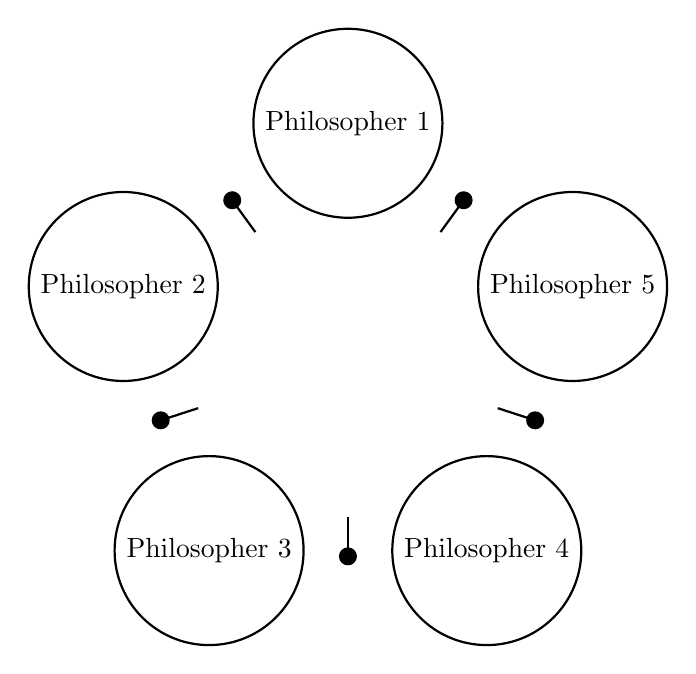
\begin{tikzpicture}

    % Draw the philosophers
    \foreach \angle/\name in {90/Philosopher 1, 162/Philosopher 2, 234/Philosopher 3, 306/Philosopher 4, 18/Philosopher 5} {
        \draw[thick] (\angle:3cm) circle (1.2cm); % Larger circle for philosophers
        \node at (\angle:3cm) {\name}; % Philosopher label
    }

    % Draw the forks between the philosophers
    \foreach \angle in {126, 198, 270, 342, 54} {
        \draw[thick] (\angle:2cm) -- (\angle:2.5cm); % Fork handle
        \draw[thick, fill=black] (\angle:2.5cm) circle (0.1cm); % Fork tip
    }

\end{tikzpicture}
\end{center}

Each philosopher is thinking or eating, but the philosopher needs to take
\textit{both} forks to eat. The problem is to design a solution that ensures one
or more philosophers can eat when they want to. \\

A possible failing scenario is when \textit{all} philosophers take the fork to
their left. Now every philosopher is stuck waiting for the fork to their right, 
and every philosopher starve.

\section{Design}

Every philosopher behaves similarly:
\begin{itemize}
    \item Take one fork 
    \item Take another fork 
    \item Eat
    \item Put away one fork
    \item Put away another fork
\end{itemize}

\section{Spec}

The core part of \textit{Spec} looks like this: 
\\
\begin{tla}
Next ==
    \/ \E k \in 0.. P-1:
        TakeFirst(k)
    \/ \E k \in 0.. P-1:
        TakeSecond(k)
    \/ \E k \in 0.. P-1:
        Eat(k)
    \/ \E k \in 0.. P-1:
        PutFirst(k)
    \/ \E k \in 0.. P-1:
        PutSecond(k)
\end{tla}
\begin{tlatex}
\@x{ Next \.{\defeq}}%
\@x{\@s{16.4} \.{\lor} \E\, k \.{\in} 0 \.{\dotdot} P \.{-} 1 \.{:}}%
\@x{\@s{20.5} TakeFirst ( k )}%
\@x{\@s{16.4} \.{\lor} \E\, k \.{\in} 0 \.{\dotdot} P \.{-} 1 \.{:}}%
\@x{\@s{20.5} TakeSecond ( k )}%
\@x{\@s{16.4} \.{\lor} \E\, k \.{\in} 0 \.{\dotdot} P \.{-} 1 \.{:}}%
\@x{\@s{20.5} Eat ( k )}%
\@x{\@s{16.4} \.{\lor} \E\, k \.{\in} 0 \.{\dotdot} P \.{-} 1 \.{:}}%
\@x{\@s{20.5} PutFirst ( k )}%
\@x{\@s{16.4} \.{\lor} \E\, k \.{\in} 0 \.{\dotdot} P \.{-} 1 \.{:}}%
\@x{\@s{20.5} PutSecond ( k )}%
\end{tlatex}
\\

This reflects the behavior described earlier. Note that there's a sequential
dependency to these actions. The philosopher can only take the second fork after
taking the first fork, eat after having both forks and put away the forks after
eating.
\\

\begin{tla}

First(k) == k
Second(k) == (k+1)% P

TakeFirst(k) == 
    /\ eaten[k] = 0
    /\ forks[First(k)] = UNUSED
    /\ UNCHANGED eaten

TakeSecond(k) ==
    /\ eaten[k] = 0
    /\ forks[First(k)] = k
    /\ forks[Second(k)] = UNUSED
    /\ forks' = [forks EXCEPT ![Second(k)] = k]
    /\ UNCHANGED eaten
\end{tla}
\begin{tlatex}
\@x{ First ( k ) \.{\defeq} k}%
\@x{ Second ( k ) \.{\defeq} ( k \.{+} 1 ) \.{\%} P}%
\@pvspace{8.0pt}%
\@x{ TakeFirst ( k ) \.{\defeq}}%
\@x{\@s{16.4} \.{\land} eaten [ k ] \.{=} 0}%
\@x{\@s{16.4} \.{\land} forks [ First ( k ) ] \.{=} UNUSED}%
\@x{\@s{16.4} \.{\land} {\UNCHANGED} eaten}%
\@pvspace{8.0pt}%
\@x{ TakeSecond ( k ) \.{\defeq}}%
\@x{\@s{16.4} \.{\land} eaten [ k ] \.{=} 0}%
\@x{\@s{16.4} \.{\land} forks [ First ( k ) ] \.{=} k}%
\@x{\@s{16.4} \.{\land} forks [ Second ( k ) ] \.{=} UNUSED}%
 \@x{\@s{16.4} \.{\land} forks \.{'} \.{=} [ forks {\EXCEPT} {\bang} [ Second
 ( k ) ] \.{=} k ]}%
\@x{\@s{16.4} \.{\land} {\UNCHANGED} eaten}%
\end{tlatex}
\\

The philosopher greedily takes the first fork when possible. After the
philosopher has the first fork, she greedily takes the second fork when
possible.
\\

\begin{tla}
Eat(k) == 
    LET 
        left == k 
        right == (k+1) % P
    IN 
        /\ forks[left] = k
        /\ forks[right] = k
        /\ eaten' = [eaten EXCEPT ![k] = 1]
        /\ UNCHANGED forks 
\end{tla}
\begin{tlatex}
\@x{ Eat ( k ) \.{\defeq}}%
\@x{ \.{\LET}}%
\@x{\@s{16.4} left \.{\defeq} k}%
\@x{\@s{16.4} right \.{\defeq} ( k \.{+} 1 ) \.{\%} P}%
\@x{ \.{\IN}}%
\@x{\@s{16.4} \.{\land} forks [ left ] \.{=} k}%
\@x{\@s{16.4} \.{\land} forks [ right ] \.{=} k}%
 \@x{\@s{16.4} \.{\land} eaten \.{'} \.{=} [ eaten {\EXCEPT} {\bang} [ k ]
 \.{=} 1 ]}%
\@x{\@s{16.4} \.{\land} {\UNCHANGED} forks}%
\end{tlatex}
\\

Once the philosopher has both forks, she can eat. 
\\
\begin{tla}
PutFirst(k) == 
    /\ eaten[k] = 1
    /\ forks[First(k)] = k 
    /\ forks' = [forks EXCEPT ![First(k)] = UNUSED]
    /\ UNCHANGED eaten

PutSecond(k) == 
    /\ eaten[k] = 1
    /\ forks[First(k)] # k 
    /\ forks[Second(k)] = k 
    /\ forks' = [forks EXCEPT ![Second(k)] = UNUSED]
    /\ eaten' = [eaten EXCEPT ![k] = 0]
\end{tla}
\begin{tlatex}
\@x{ PutFirst ( k ) \.{\defeq}}%
\@x{\@s{16.4} \.{\land} eaten [ k ] \.{=} 1}%
\@x{\@s{16.4} \.{\land} forks [ First ( k ) ] \.{=} k}%
 \@x{\@s{16.4} \.{\land} forks \.{'} \.{=} [ forks {\EXCEPT} {\bang} [ First (
 k ) ] \.{=} UNUSED ]}%
\@x{\@s{16.4} \.{\land} {\UNCHANGED} eaten}%
\@pvspace{8.0pt}%
\@x{ PutSecond ( k ) \.{\defeq}}%
\@x{\@s{16.4} \.{\land} eaten [ k ] \.{=} 1}%
\@x{\@s{16.4} \.{\land} forks [ First ( k ) ] \.{\neq} k}%
\@x{\@s{16.4} \.{\land} forks [ Second ( k ) ] \.{=} k}%
 \@x{\@s{16.4} \.{\land} forks \.{'} \.{=} [ forks {\EXCEPT} {\bang} [ Second
 ( k ) ] \.{=} UNUSED ]}%
 \@x{\@s{16.4} \.{\land} eaten \.{'} \.{=} [ eaten {\EXCEPT} {\bang} [ k ]
 \.{=} 0 ]}%
\end{tlatex}
\\

After eating, the philosopher puts away the forks.

\section{Safety}

Omitted for this chapter.

\section{Liveness}

One liveness property is to ensure that at least one philosopher can eat when she
wants to under all circumstances:\\

\begin{tla}
Liveness ==
    \E k \in 0..P-1:
        /\ eaten[k] = 0 ~> eaten[k] = 1
        /\ eaten[k] = 1 ~> eaten[k] = 0
\end{tla}
\begin{tlatex}
\@x{ Liveness \.{\defeq}}%
\@x{\@s{16.4} \E\, k \.{\in} 0 \.{\dotdot} P \.{-} 1 \.{:}}%
\@x{\@s{20.5} \.{\land} eaten [ k ] \.{=} 0 \.{\leadsto} eaten [ k ] \.{=} 1}%
\@x{\@s{20.5} \.{\land} eaten [ k ] \.{=} 1 \.{\leadsto} eaten [ k ] \.{=} 0}%
\end{tlatex}
\\

However, \textit{Spec} defined as is doesn't implement any deadlock mitigation.
Running it against the model the checker results in the following violations: 

\begin{verbatim}
State 2: <TakeFirst line 19, col 5 to line 23, 
    col 22 of module dining>
/\ eaten = (0 :> 0 @@ 1 :> 0 @@ 2 :> 0)
/\ forks = (0 :> 0 @@ 1 :> 100 @@ 2 :> 100)

State 3: <TakeFirst line 19, col 5 to line 23, 
    col 22 of module dining>
/\ eaten = (0 :> 0 @@ 1 :> 0 @@ 2 :> 0)
/\ forks = (0 :> 0 @@ 1 :> 1 @@ 2 :> 100)

State 4: <TakeFirst line 19, col 5 to line 23, 
    col 22 of module dining>
/\ eaten = (0 :> 0 @@ 1 :> 0 @@ 2 :> 0)
/\ forks = (0 :> 0 @@ 1 :> 1 @@ 2 :> 2)
\end{verbatim}

When all philosopher takes their left fork, no one can eat. \\

A simple fix to the problem is for every philosopher to take the fork with the
smaller index first:\\

\begin{tla}
First(k) == IF k # P-1 THEN k ELSE 0
Second(k) == IF k # P-1 THEN k+1 ELSE k
\end{tla}
\begin{tlatex}
 \@x{ First ( k ) \.{\defeq} {\IF} k \.{\neq} P \.{-} 1 \.{\THEN} k \.{\ELSE}
 0}%
 \@x{ Second ( k ) \.{\defeq} {\IF} k \.{\neq} P \.{-} 1 \.{\THEN} k \.{+} 1
 \.{\ELSE} k}%
\end{tlatex}
\\

When the philosopher with the highest index wants to eat, she will need to take
fork 0 first. In the case where all other philosophers have already taken their
first fork, the philosopher with the highest index will fail to take her first
fork (because it has already been taken by the first philosopher). This allows
the philosopher with the second-highest index to make progress, thus preventing a
deadlock.\\

The model checker will pass the updated \textit{Spec}.

% \end{document}


% \begin{document}

\chapter{Strongly Connected Components}

In a graph, a strongly connected component (SCC) is a subset of vertices where
every pair of vertices are reachable from each other. An example graph with four
SCCs is illustrated below, where the vertices that share the same color and belong in the
same SCC:\\

\begin{center}
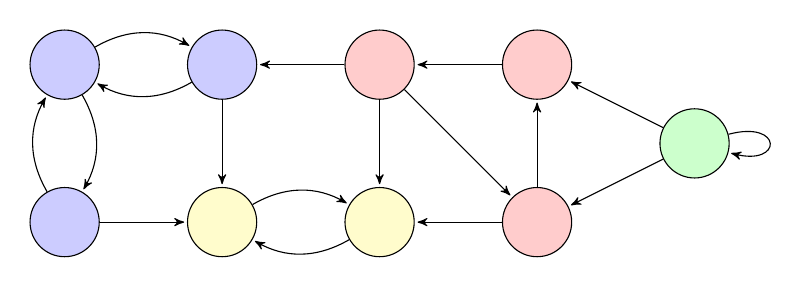
\begin{tikzpicture}[->, >=stealth', shorten >=1pt, auto, node distance=2cm]

  % Define nodes

  \node[state, fill=blue!20] (n1) at (0, 0)  {};
  \node[state, fill=blue!20] (n2) at (0, -2) {};
  \node[state, fill=blue!20] (n3) at (2, 0)  {};

  \node[state, fill=yellow!20] (n4) at (2, -2) {};

  \node[state, fill=red!20] (n5) at (4, 0)  {};
  \node[state, fill=yellow!20] (n6) at (4, -2) {};

  \node[state, fill=red!20] (n7) at (6, 0)  {};
  \node[state, fill=red!20] (n8) at (6, -2) {};

  \node[state, fill=green!20] (n9) at (8, -1) {};

  % Draw edges
  \draw[->] (n1) edge[bend left] (n2);
  \draw[->] (n2) edge[bend left] (n1);

  \draw[->] (n1) edge[bend left] (n3);
  \draw[->] (n3) edge[bend left] (n1);

  \draw[->] (n3) edge[] (n4);
  \draw[->] (n2) edge[] (n4);

  \draw[->] (n4) edge[bend left] (n6);
  \draw[->] (n6) edge[bend left] (n4);

  \draw[->] (n5) edge[] (n3);
  \draw[->] (n5) edge[] (n6);
  \draw[->] (n5) edge[] (n8);

  \draw[->] (n7) edge[] (n5);

  \draw[->] (n8) edge[] (n6);
  \draw[->] (n8) edge[] (n7);

  \draw[->] (n9) edge[] (n7);
  \draw[->] (n9) edge[] (n8);
  
  \draw[->] (n9) edge[loop right] (n9);

\end{tikzpicture}
\end{center}

A node is an SCC by itself. There are many applications of SCCs, including:
social network analysis, web crawling, and software modularity analysis.\\

TLA+ also uses SCCs to verify the liveness properties of a specification.
Consider the following graph from a hypothetical specification: 

\begin{center}
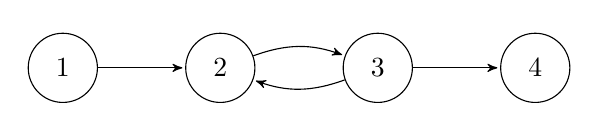
\begin{tikzpicture}[>=stealth',shorten >=1pt,auto,node distance=2cm]
  \node[state]  (q1)                {1};
  \node[state]  (q2) [right of=q1]  {2};
  \node[state]  (q3) [right of=q2]  {3};
  \node[state]  (q4) [right of=q3]  {4};

  \path[->]          (q1) edge   []   node {} (q2);

  \path[->]          (q2) edge   [bend left=20]   node {} (q3);
  \path[->]          (q3) edge   [bend left=20]   node {} (q2);
  
  \path[->]          (q3) edge   []   node {} (q4);
\end{tikzpicture}
\end{center}

States 2 and 3 form an SCC. Assume the system has a liveness property that
defines state 1 \textit{leads to} state 4. The model checker can fail the specification
because execution may be trapped inside the SSC (unless a fairness description
is provided). The model checker must first identify all SCCs in the graph to
verify liveness. This explains why verifying liveness non-trivially increases
model checker runtime, because the SCC identifying algorithm implemented in the
model checker runs linearly.\\

In this chapter, we will implement a horizontally scalable SCC detection
algorithm described in \textit{A GPU Algorithm for Detecting Strongly Connected
Components} \cite{gpu_scc}.

\section{Design}

The following provides the pseudocode description of the parallel SCC detection
algorithm as described in the paper:\\

\makeatletter
\algnewcommand{\LineComment}[1]{\Statex \hskip\ALG@thistlm \(\triangleright\) #1}
\makeatother

\begin{algorithmic}[1]

\State $converged \gets false$

\While{not $converged$}
    
    \LineComment{Initialize vertex}
    \ForAll{vertices $v \in V$}
        \State $v_{in} \gets v_{id}$
        \State $v_{out} \gets v_{id}$
    \EndFor

    \LineComment{Propagate max value}
    \State $updated \gets false$
    \While{$updated$}
        \ForAll{edges $(u -> v)\in E$}
            \State $v_{out} \gets max(u_{out},v_{out})$
            \State $v_{in} \gets max(u_{in},v_{in})$
        \EndFor
        \State $updated \gets$ at least one $v_{in}$ or $v_{out}$ value changed 
    \EndWhile

    \LineComment{Remove edges that span SCC}
    \ForAll{edges $(u \rightarrow v)\in E$}
        \If {$u_{in} \neq v_{in}$ or $u_{out} \neq v_{out}$}
            \State $E \gets E \ (u \rightarrow v)$
        \EndIf
    \EndFor

\EndWhile
\end{algorithmic}

The algorithm is split into three parts: initialization, max value
propagation and edge trimming.

\section{Specification}

\textit{Spec} is defined into three phases: \textit{Init}, \textit{Update},
\textit{Trim}. Phase \textit{Init} is defined as follow:\\
\begin{tla}
PhaseInit == 
    /\ phase = "Init" 
    /\ phase' = "Update"
    /\ edges' = new_edges
    /\ new_edges' = new_edges
    /\ in' = [k \in Vertex |-> k]
    /\ out' = [k \in Vertex |-> k]
    /\ updated' = 0
    /\ converged' = 0
\end{tla}
\begin{tlatex}
\@x{ PhaseInit \.{\defeq}}%
\@x{\@s{16.4} \.{\land} phase \.{=}\@w{Init}}%
\@x{\@s{16.4} \.{\land} phase \.{'} \.{=}\@w{Update}}%
\@x{\@s{16.4} \.{\land} edges \.{'} \.{=} new\_edges}%
\@x{\@s{16.4} \.{\land} new\_edges \.{'} \.{=} new\_edges}%
\@x{\@s{16.4} \.{\land} in \.{'} \.{=} [ k \.{\in} Vertex \.{\mapsto} k ]}%
\@x{\@s{16.4} \.{\land} out \.{'} \.{=} [ k \.{\in} Vertex \.{\mapsto} k ]}%
\@x{\@s{16.4} \.{\land} updated \.{'} \.{=} 0}%
\@x{\@s{16.4} \.{\land} converged \.{'} \.{=} 0}%
\end{tlatex}\\

\textit{in} and \textit{out} are defined as lookup table using
\textit{functions}.\\

\pagebreak

The \textit{Update} phase implements max value propagation:\\
\begin{tla}
PhaseUpdate == 
    /\ phase = "Update"
    /\ \/ /\ \E e \in edges: 
            LET 
                src == e[1]
                dst == e[2]
            IN 
                /\ in' = [in EXCEPT ![dst] = Max(in[src], in[dst])]
                /\ out' = [out EXCEPT ![src] = Max(out[src], out[dst])]
                /\ edges' = edges \ {e}
                /\ \/ /\ in' # in \/ out' # out
                      /\ updated' = 1
                   \/ /\ in' = in /\ out' = out
                      /\ updated' = 0
          /\ UNCHANGED <<new_edges, phase, converged>>
       \/ /\ edges = {}
          /\ updated = 0
          /\ phase' = "Trim"
          /\ UNCHANGED <<edges, new_edges, in, out, updated, converged>>
       \/ /\ edges = {}
          /\ updated # 0
          /\ edges' = new_edges
          /\ UNCHANGED <<phase, new_edges, in, out, updated, converged>>
\end{tla}
\begin{tlatex}
\@x{ PhaseUpdate \.{\defeq}}%
\@x{\@s{16.4} \.{\land} phase \.{=}\@w{Update}}%
\@x{\@s{16.4} \.{\land} \.{\lor} \.{\land} \E\, e \.{\in} edges \.{:}}%
\@x{\@s{24.59} \.{\LET}}%
\@x{\@s{41.0} src \.{\defeq} e [ 1 ]}%
\@x{\@s{41.0} dst \.{\defeq} e [ 2 ]}%
\@x{\@s{24.59} \.{\IN}}%
 \@x{\@s{41.0} \.{\land} in \.{'} \.{=} [ in {\EXCEPT} {\bang} [ dst ] \.{=}
 Max ( in [ src ] ,\, in [ dst ] ) ]}%
 \@x{\@s{41.0} \.{\land} out \.{'} \.{=} [ out {\EXCEPT} {\bang} [ src ] \.{=}
 Max ( out [ src ] ,\, out [ dst ] ) ]}%
\@x{\@s{41.0} \.{\land} edges \.{'} \.{=} edges \.{\,\backslash\,} \{ e \}}%
 \@x{\@s{41.0} \.{\land} \.{\lor} \.{\land} in \.{'} \.{\neq} in \.{\lor} out
 \.{'} \.{\neq} out}%
\@x{\@s{41.0} \.{\land} updated \.{'} \.{=} 1}%
 \@x{\@s{41.0} \.{\lor} \.{\land} in \.{'} \.{=} in \.{\land} out \.{'} \.{=}
 out}%
\@x{\@s{41.0} \.{\land} updated \.{'} \.{=} 0}%
 \@x{\@s{16.4} \.{\land} {\UNCHANGED} {\langle} new\_edges ,\, phase ,\,
 converged {\rangle}}%
\@x{\@s{16.4} \.{\lor} \.{\land} edges \.{=} \{ \}}%
\@x{\@s{16.4} \.{\land} updated \.{=} 0}%
\@x{\@s{16.4} \.{\land} phase \.{'} \.{=}\@w{Trim}}%
 \@x{\@s{16.4} \.{\land} {\UNCHANGED} {\langle} edges ,\, new\_edges ,\, in
 ,\, out ,\, updated ,\, converged {\rangle}}%
\@x{\@s{16.4} \.{\lor} \.{\land} edges \.{=} \{ \}}%
\@x{\@s{16.4} \.{\land} updated \.{\neq} 0}%
\@x{\@s{16.4} \.{\land} edges \.{'} \.{=} new\_edges}%
 \@x{\@s{16.4} \.{\land} {\UNCHANGED} {\langle} phase ,\, new\_edges ,\, in
 ,\, out ,\, updated ,\, converged {\rangle}}%
\end{tlatex}
\\

The edge iteration loop is implemented with an existential qualifier over edges.
After processing an edge, the edge is removed from the set edges to simulate so
it is not chosen again in the next iteration. Once set edges become empty, the
algorithm determines if we need to repeat the propagation process.\\

\pagebreak

The following implements phase \textit{trim}:\\
\begin{tla}
PhaseTrim == 
    /\ phase = "Trim"
    /\ \/ /\ edges = {}
          /\ in = out
          /\ converged' = 1
          /\ UNCHANGED <<phase, new_edges, edges, in, out, updated>>
       \/ /\ edges = {}
          /\ in # out
          /\ phase' = "Init"
          /\ UNCHANGED <<in, new_edges, edges, out, updated, converged>>
       \/ /\ edges # {}
          /\ \E e \in edges:
            LET 
                src == e[1]
                dst == e[2]
            IN
                /\ \/ /\ out[src] # out[dst] \/ in[src] # in[dst]
                      /\ new_edges' = new_edges \ {e}
                   \/ /\ out[src] = out[dst] /\ in[src] = in[dst]
                      /\ UNCHANGED new_edges
                /\ edges' = edges \ {e}
          /\ UNCHANGED <<phase, in, out, updated, converged>>
\end{tla}
\begin{tlatex}
\@x{ PhaseTrim \.{\defeq}}%
\@x{\@s{16.4} \.{\land} phase \.{=}\@w{Trim}}%
\@x{\@s{16.4} \.{\land} \.{\lor} \.{\land} edges \.{=} \{ \}}%
\@x{\@s{16.4} \.{\land} in \.{=} out}%
\@x{\@s{16.4} \.{\land} converged \.{'} \.{=} 1}%
 \@x{\@s{16.4} \.{\land} {\UNCHANGED} {\langle} phase ,\, new\_edges ,\, edges
 ,\, in ,\, out ,\, updated {\rangle}}%
\@x{\@s{16.4} \.{\lor} \.{\land} edges \.{=} \{ \}}%
\@x{\@s{16.4} \.{\land} in \.{\neq} out}%
\@x{\@s{16.4} \.{\land} phase \.{'} \.{=}\@w{Init}}%
 \@x{\@s{16.4} \.{\land} {\UNCHANGED} {\langle} in ,\, new\_edges ,\, edges
 ,\, out ,\, updated ,\, converged {\rangle}}%
\@x{\@s{16.4} \.{\lor} \.{\land} edges \.{\neq} \{ \}}%
\@x{\@s{16.4} \.{\land} \E\, e \.{\in} edges \.{:}}%
\@x{\@s{24.59} \.{\LET}}%
\@x{\@s{41.0} src \.{\defeq} e [ 1 ]}%
\@x{\@s{41.0} dst \.{\defeq} e [ 2 ]}%
\@x{\@s{24.59} \.{\IN}}%
 \@x{\@s{41.0} \.{\land} \.{\lor} \.{\land} out [ src ] \.{\neq} out [ dst ]
 \.{\lor} in [ src ] \.{\neq} in [ dst ]}%
 \@x{\@s{41.0} \.{\land} new\_edges \.{'} \.{=} new\_edges \.{\,\backslash\,}
 \{ e \}}%
 \@x{\@s{41.0} \.{\lor} \.{\land} out [ src ] \.{=} out [ dst ] \.{\land} in [
 src ] \.{=} in [ dst ]}%
\@x{\@s{41.0} \.{\land} {\UNCHANGED} new\_edges}%
\@x{\@s{41.0} \.{\land} edges \.{'} \.{=} edges \.{\,\backslash\,} \{ e \}}%
 \@x{\@s{16.4} \.{\land} {\UNCHANGED} {\langle} phase ,\, in ,\, out ,\,
 updated ,\, converged {\rangle}}%
\end{tlatex}
\\

Similar to the previous phase, we use existential qualifiers and set subtraction to
simulate iterating through all edges. Another variable \textit{new\_edges} is
used to track edges to be used in the next iteration if required. 

\section{Safety}

To find the solution of a given graph, let us define a safety property where
converged is always 0:\\

\begin{tla}
Termination == 
    converged = 0
\end{tla}
\begin{tlatex}
\@x{ Termination \.{\defeq}}%
\@x{\@s{16.4} converged \.{=} 0}%
\end{tlatex}

In other words, we want the model checker to terminate when converged becomes 1.\\ 

Let us assume input similar to as defined in the paper:

\begin{center}
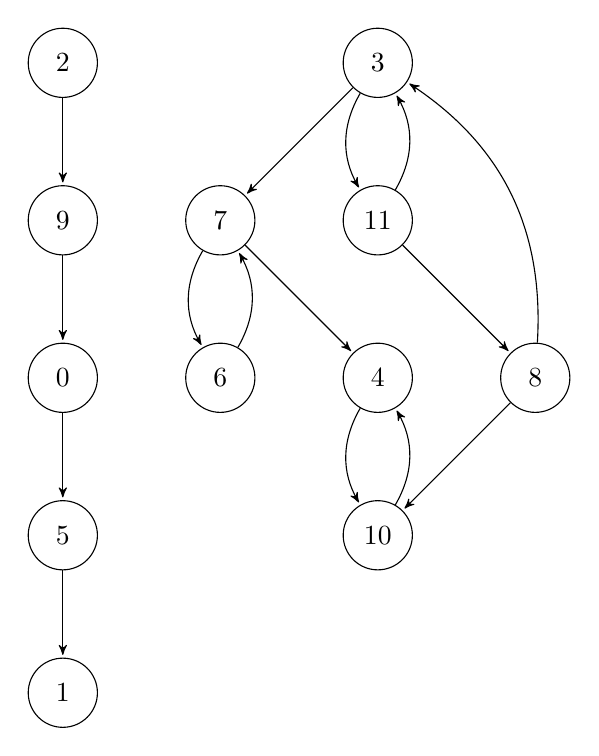
\begin{tikzpicture}[->, >=stealth', shorten >=1pt, auto, node distance=2cm]

  % Define nodes

  \node[state] (n2) at (0, 0)  {2};
  \node[state] (n9) at (0, -2) {9};
  \node[state] (n0) at (0, -4) {0};
  \node[state] (n5) at (0, -6) {5};
  \node[state] (n1) at (0, -8) {1};

  \node[state] (n3) at (4, 0) {3};
  \node[state] (n11) at (4, -2) {11};
  \node[state] (n7) at (2, -2) {7};
  \node[state] (n4) at (4, -4) {4};
  \node[state] (n6) at (2, -4) {6};
  \node[state] (n10) at (4, -6) {10};
  \node[state] (n8) at (6, -4) {8};

  % Draw edges
  \draw[->] (n2) edge[] (n9);
  \draw[->] (n9) edge[] (n0);
  \draw[->] (n0) edge[] (n5);
  \draw[->] (n5) edge[] (n1);

  \draw[->] (n3) edge[] (n7);
  \draw[->] (n3) edge[bend right] (n11);

  \draw[->] (n6) edge[bend right] (n7);

  \draw[->] (n7) edge[bend right] (n6);
  \draw[->] (n7) edge[] (n4);

  \draw[->] (n8) edge[] (n10);
  \draw[->] (n8) edge[bend right] (n3);

  \draw[->] (n4) edge[bend right] (n10);

  \draw[->] (n10) edge[bend right] (n4);

  \draw[->] (n11) edge[] (n8);
  \draw[->] (n11) edge[bend right] (n3);

%   \draw[->] (n2) edge[bend left] (n1);

%   \draw[->] (n1) edge[bend left] (n3);
%   \draw[->] (n3) edge[bend left] (n1);

%   \draw[->] (n3) edge[] (n4);
%   \draw[->] (n2) edge[] (n4);

%   \draw[->] (n4) edge[bend left] (n6);
%   \draw[->] (n6) edge[bend left] (n4);

%   \draw[->] (n5) edge[] (n3);
%   \draw[->] (n5) edge[] (n6);
%   \draw[->] (n5) edge[] (n8);

%   \draw[->] (n7) edge[] (n5);

%   \draw[->] (n8) edge[] (n6);
%   \draw[->] (n8) edge[] (n7);

%   \draw[->] (n9) edge[] (n7);
%   \draw[->] (n9) edge[] (n8);
  
%   \draw[->] (n9) edge[loop right] (n9);

\end{tikzpicture}
\end{center}

Running the model checker against the specification outputs the following: 
\begin{verbatim}
Error: Invariant Termination is violated.                               
Error: The behavior up to this point is:      
...
State 15: <PhaseTrim line 76, col 5 to line 96, 
    col 61 of module scc>
/\ out = ( 0 :> 0 @@ 
  1 :> 1 @@  
  2 :> 2 @@ 
  3 :> 11 @@                                                            
  4 :> 10 @@                                                            
  5 :> 5 @@                                                             
  6 :> 7 @@                                                             
  7 :> 7 @@                                                             
  8 :> 11 @@                                                            
  9 :> 9 @@                                                             
  10 :> 10 @@                                                           
  11 :> 11 )   
...
\end{verbatim}

As defined by the algorithm, vertices sharing the same value are part of the
same SCC. The specification correctly identifies three SCCs with more than one vertex:
\{3, 8, 11\}, \{6, 7\} and \{4, 10\}.

\section{Liveness}

Omitted for this chapter.

% \end{document}


SPECIFICATION Spec

INVARIANTS 
    \* TypeOK
PROPERTIES 
    \* Liveness


% \begin{document}

\chapter{Simple Gossip Protocol}

In a distributed system, a cluster of nodes collectively provides a service. A
distributed system may have 10s to 100s of nodes working together to offer the
service in a geo-diverse environment to maximize uptime. The nodes often
have requirements to know about each other. In the context of a distributed
database, a node may need to know the key range of another of its peers. The
cluster needs a way to communicate this information. One such mechanism is the
gossip protocol.\newline

Gossip protocol allows nodes to fetch the latest cluster information in a
distributed fashion. Before the gossip protocol, nodes in a cluster learn about
their neighbors by contacting a centralized server. This introduces a single
failure point in the system. Gossip protocol relies on nodes to initiate
the data exchange, and the nodes in the cluster periodically select a set of neighbors to
gossip with. \newline

Assume an N node cluster, at some periodic interval a node selects k neighbors
to gossip with. The total amount of gossip propagation time is described
logarithmically below:

\begin{center}
$propagation\_time = \log_k N * gossip\_interval$
\end{center}

With the total number of messages exchanged:
\begin{center}
$messages\_exchanged = \log_k N * k$
\end{center}

\section{Design}

In this chapter, we will implement a simplified gossip model where: 
\begin{itemize}
    \item Each node has a version.
    \item Each node caches the version of all other nodes.
    \item A pair of nodes are randomly selected to gossip 
    \item A node can restart. Restarting a node clears the node's version cache
    of the other nodes.
    \item A node can bump its version.
\end{itemize}

If the gossip protocol works correctly, every node should eventually have the
the latest version of all the nodes.

\section{Spec}

In gossip protocol, every node needs to remember all its peer's current
version:\newline

\begin{tla}
Init ==
    /\ version = [i \in Servers |-> [j \in Servers |-> 0]]
Next ==
    \/ \E i \in Servers:
        /\ Bump(i)
    \/ \E i, j \in Servers:
        /\ Gossip(i, j)
    \/ \E i \in Servers:
        /\ Restart(i)
\end{tla}
\begin{tlatex}
\@x{ Init \.{\defeq}}%
 \@x{\@s{16.4} \.{\land} version \.{=} [ i \.{\in} Servers \.{\mapsto} [ j
 \.{\in} Servers \.{\mapsto} 0 ] ]}%
\@x{ Next \.{\defeq}}%
\@x{\@s{16.4} \.{\lor} \E\, i \.{\in} Servers \.{:}}%
\@x{\@s{20.5} \.{\land} Bump ( i )}%
\@x{\@s{16.4} \.{\lor} \E\, i ,\, j \.{\in} Servers \.{:}}%
\@x{\@s{20.5} \.{\land} Gossip ( i ,\, j )}%
\@x{\@s{16.4} \.{\lor} \E\, i \.{\in} Servers \.{:}}%
\@x{\@s{20.5} \.{\land} Restart ( i )}%
\end{tlatex}
\newline

The \textit{Init} formula simply declares the version to be a two-dimensional array
with all elements initialized to 0. \textit{Next} allows either bumping the version
of a server, picking a pair of nodes to gossip, or restarting a server.\newline

The following defines these steps:\newline

\begin{tla}
Gossip(i, j) == 
    LET 
        Max(a, b) == IF a > b THEN a ELSE b
        updated == [k \in Servers |-> Max(version[i][k], version[j][k])]
        version_a == [version EXCEPT ![i] = updated]
        version_ab == [version_a EXCEPT ![j] = updated]
    IN 
        /\ version' = version_ab 
\end{tla}
\begin{tlatex}
\@x{ Gossip ( i ,\, j ) \.{\defeq}}%
\@x{\@s{16.4} \.{\LET}}%
 \@x{\@s{32.8} Max ( a ,\, b ) \.{\defeq} {\IF} a \.{>} b \.{\THEN} a
 \.{\ELSE} b}%
 \@x{\@s{32.8} updated \.{\defeq} [ k \.{\in} Servers \.{\mapsto} Max (
 version [ i ] [ k ] ,\, version [ j ] [ k ] ) ]}%
 \@x{\@s{32.8} version\_a \.{\defeq} [ version {\EXCEPT} {\bang} [ i ] \.{=}
 updated ]}%
 \@x{\@s{32.8} version\_ab \.{\defeq} [ version\_a {\EXCEPT} {\bang} [ j ]
 \.{=} updated ]}%
\@x{\@s{16.4} \.{\IN}}%
\@x{\@s{32.8} \.{\land} version \.{'} \.{=} version\_ab}%
\end{tlatex}
\newline

When two servers gossip, they gossip about all the nodes (including themselves)
and update both of their version cache with the more up-to-date entry between
the two. The \textit{LET..IN} syntax enables local macro definition. In this
example, we use temporary variables defined inside \textit{LET}, and update the
primed variable inside the \textit{IN} clause.\newline

\begin{tla}
Bump(i) == 
    /\ version[i][i] # MaxVersion 
    /\ version' = [version EXCEPT ![i] = [k \in Servers |-> 
        IF i # k THEN version[i][k] ELSE version[i][k] + 1]]
\end{tla}
\begin{tlatex}
\@x{ Bump ( i ) \.{\defeq}}%
\@x{ \.{\land} version [ i ] [ i ] \.{\neq} MaxVersion}%
 \@x{ \.{\land} version \.{'} \.{=} [ version {\EXCEPT} {\bang} [ i ] \.{=} [
 k \.{\in} Servers \.{\mapsto}}%
 \@x{\@s{4.1} {\IF} i \.{\neq} k \.{\THEN} version [ i ] [ k ] \.{\ELSE}
 version [ i ] [ k ] \.{+} 1 ] ]}%
\end{tlatex}
\newline

The action only permits version bump if the Server hasn't made it to 
\textit{MaxVersion}. When the Server bumps the version, it only bumps its 
version and keeps all other versions in its version cache as is. \newline
\begin{tla}
Restart(i) == 
    /\ version' = [version EXCEPT ![i] = [k \in Servers |-> 
        IF i # k THEN 0 ELSE version[i][i]]]
\end{tla}
\begin{tlatex}
\@x{ Restart ( i ) \.{\defeq}}%
 \@x{\@s{16.4} \.{\land} version \.{'} \.{=} [ version {\EXCEPT} {\bang} [ i ]
 \.{=} [ k \.{\in} Servers \.{\mapsto}}%
 \@x{\@s{20.5} {\IF} i \.{\neq} k \.{\THEN} 0 \.{\ELSE} version [ i ] [ i ] ]
 ]}%
\end{tlatex}
\newline

Upon \textit{Restart}, a server reloads from its local storage (so its version persists), but the server needs to re-learn the cluster status (all other
entries in its version cache are wiped).\newline

\textit{Spec} defines three actions: \textit{Bump}, \textit{Restart},
\textit{Gossip}. Without any fairness description, \textit{Any} permutation of
these actions are allowed by the Spec, and \textit{will} be checked by the model
checker:
\begin{itemize}
    \item Restart, Restart, Restart,...
    \item Bump, Bump, Bump, Bump ...
    \item Restart, Gossip, Restart, Gossip, ... 
\end{itemize}

We will discuss how to specify fairness in the Liveness section of this chapter.

\section{Safety}

\section{Liveness}

The expected behavior of a system using gossip protocol is to ensure the
cluster converges towards a higher version number for all servers even in the
presence of failure (represented by \textit{Restart}). This means we need to
guarantee \textit{Bump} is always being called. Without this guarantee, the Spec
can trap in a \textit{Restart} and \textit{Gossip} loop. To ensure \textit{Bump}
is always called, we need to add fairness description:\\

\begin{tla}
Spec ==
  /\ Init
  /\ [][Next]_vars
  /\ WF_vars(Next)
  /\ \A i \in Servers: 
    WF_vars(Bump(i))
\end{tla}
\begin{tlatex}
\@x{ Spec \.{\defeq}}%
\@x{\@s{8.2} \.{\land} Init}%
\@x{\@s{8.2} \.{\land} {\Box} [ Next ]_{ vars}}%
\@x{\@s{8.2} \.{\land} {\WF}_{ vars} ( Next )}%
\@x{\@s{8.2} \.{\land} \A\, i \.{\in} Servers \.{:}}%
\@x{\@s{16.4} {\WF}_{ vars} ( Bump ( i ) )}%
\end{tlatex}
\\

The model checker explores all possible transitions permitted by \textit{Spec}.
This includes calling Restart repeatedly, calling Gossip, and calling any
subset of the actions repeatedly. The fairness description guarantees that if
the enabling condition of an action is true, the action will be taken. If the system
is trapped in a Restart and Gossip loop when Bump can be called, specifying fairness 
for Bump ensures Bump is called, breaking the loop.\newline

With the Spec ensuring the system always migrate towards higher version number, 
we can now define the Liveness property:\newline

\begin{tla}
Liveness == 
    \E i, j \in Servers: 
        /\ i # j
        /\ []<>(version[i][i] = MaxVersion
             /\ version[i][i] = MaxVersion 
             /\ version[i][j] = MaxVersion)
\end{tla}
\begin{tlatex}
\@x{ Liveness \.{\defeq}}%
\@x{\@s{16.4} \E\, i ,\, j \.{\in} Servers \.{:}}%
\@x{\@s{16.4} \.{\land} i \.{\neq} j}%
 \@x{\@s{16.4} \.{\land} {\Box} {\Diamond} ( version [ i ] [ i ] \.{=}
 MaxVersion}%
\@x{\@s{16.4} \.{\land} version [ i ] [ i ] \.{=} MaxVersion}%
\@x{\@s{16.4} \.{\land} version [ i ] [ j ] \.{=} MaxVersion )}%
\end{tlatex}
\\

The $\Box\Diamond$ represents \textit{always eventually}. The liveness condition
specifies that there exists a pair of Servers such that both of them
\textit{always eventually} make it to MaxVersion and have Gossip with each
other.\\

Since the Spec permits \textit{Restart} to be called anytime, a liveness
property where \textit{all} Servers are up-to-date cannot be true. The model
checker can always \textit{Restart} one of the Servers before this property is
met.\\

Likewise, replacing \textit{always eventually} with \textit{eventually always}
($\Diamond\Box$) also fails. $\Diamond\Box$ checks that once the system
\textit{eventually} enters a specified state, it \textit{always} remains in that
state. This cannot be true as the liveness condition is transient, since the
model checker can always disturb any condition with a \textit{Restart}.\\

For a more comprehensive discussion of fairness, refer to the last section of
the book.

% \end{document}


% \begin{document}

\chapter{Selective Retransmit}

Assume a client device that plays a video stream. Structurally, a video is
composed of frames, frames are then segmented into packets to stream across a
network. The client device recombines the packets into a frame and then sequences the frame to playback the video.\newline

However, the network is not-deterministic. Depending on the route the packets take
to get to the client, they may arrive out-of-order. The client may need to
maintain a receive buffer for the packets and re-order the packets back into
sequence before pushing the packets down to the decoding engine.\newline

The network may also drop packets if any of the switches along the way get
busy. In the case of a packet drop, the client has a few options. The client can
either discard the frame and let the decoding engine downstream deal with it
(which may result in visible artifacts during playback). The client can
request the whole frame to be re-sent, which results in additional bandwidth consumption.  The client can selectively request the missing packet to be
retransmitted, which will minimize additional bandwidth consumption but
increase implementation complexity.\newline

In this chapter, we will implement a simple selective retransmit
algorithm.\newline

\begin{center}

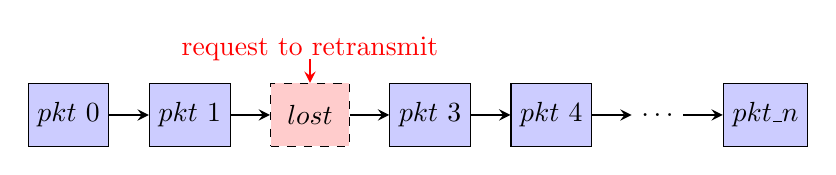
\begin{tikzpicture}[
    packet/.style={rectangle, draw, fill=blue!20, minimum width=1cm, minimum height=0.8cm},
    missing/.style={rectangle, draw, dashed, fill=red!20, minimum width=1cm, minimum height=0.8cm},
    arrow/.style={->, >=stealth, thick}
]

    % Draw packets
    \node[packet] (p0) at (0,0) {\(pkt\ 0\)};
    \node[packet, right=0.5cm of p0] (p2) {\(pkt\ 1\)};
    \node[missing, right=0.5cm of p2] (missing1) {\(lost\)};
    \node[packet, right=0.5cm of missing1] (p4) {\(pkt\ 3\)};
    \node[packet, right=0.5cm of p4] (p5) {\(pkt\ 4\)};
    \node[right=0.5cm of p5] (dots) {\(\dots\)}; % Just dots, no box
    \node[packet, right=0.5cm of dots] (pn) {\(pkt\_n\)};

    % Draw arrows between packets
    \draw[arrow] (p0.east) -- (p2.west);
    \draw[arrow] (p2.east) -- (missing1.west);
    \draw[arrow] (missing1.east) -- (p4.west);
    \draw[arrow] (p4.east) -- (p5.west);
    \draw[arrow] (p5.east) -- (dots);
    \draw[arrow] (dots) -- (pn.west);

    % Add arrow pointing to "lost" with caption
    \draw[arrow, red] ([yshift=0.3cm] missing1.north) -- (missing1.north) 
        node[midway, above, text=red] {request to retransmit};

\end{tikzpicture}

\end{center}

Since packets may arrive out-of-order, the server stamps the packets with
sequence number to allow the client to order the packets as they arrive.
Once the client has a set of ordered packets, it moves the packets from the 
receive buffer into the decoding engine to be displayed.\newline

The video packets are often sent via unreliable channel to minimize network
overhead and latency. The client sends acknowledgement back to the server to
acknowledge the received packet. This indicates to the server it can send more
video data to the client. Acknowlegements are not latency sensitive in
nature, and take up a very small proportion of bandwidth, so they are
transported through reliable channel.\newline

The following illustrates packet reorder handling:
\begin{center}
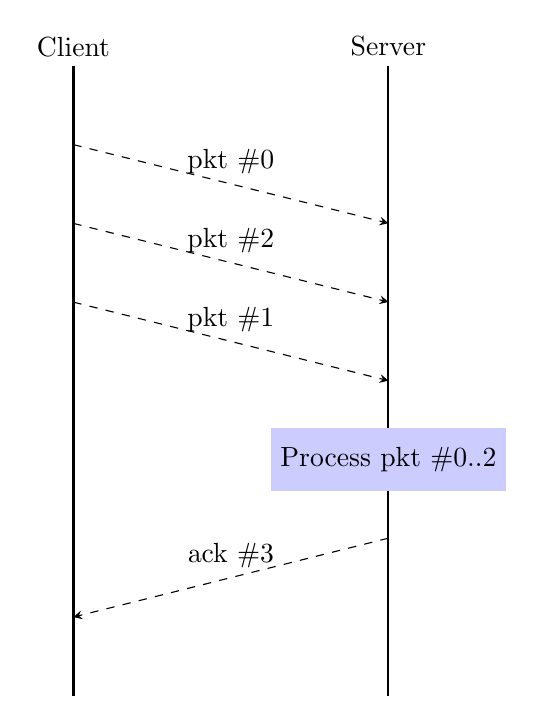
\begin{tikzpicture}[
    lifeline/.style={thick},
    message/.style={->, >=stealth, dashed},
    activation/.style={rectangle, fill=blue!20, minimum width=0.5cm, minimum height=0.8cm} ]

    \node[] (client) at (0,0) {Client};
    \node[] (server) at (4,0) {Server};

    \draw[lifeline] (client.south) -- ++(0,-8);
    \draw[lifeline] (server.south) -- ++(0,-8);

    \draw[message] ([yshift=-1cm] client.south) -- node[above] {pkt \#0} ([yshift=-2cm] server.south);
    \draw[message] ([yshift=-2cm] client.south) -- node[above] {pkt \#2} ([yshift=-3cm] server.south);
    \draw[message] ([yshift=-3cm] client.south) -- node[above] {pkt \#1} ([yshift=-4cm] server.south);
    \draw[message] ([yshift=-6cm] server.south) -- node[above] {ack \#3} ([yshift=-7cm] client.south);

    \node[activation] at ([yshift=-5cm] server.south) {Process pkt \#0..2};
\end{tikzpicture}
\end{center}

The following illustrates packet loss handling:
\begin{center}
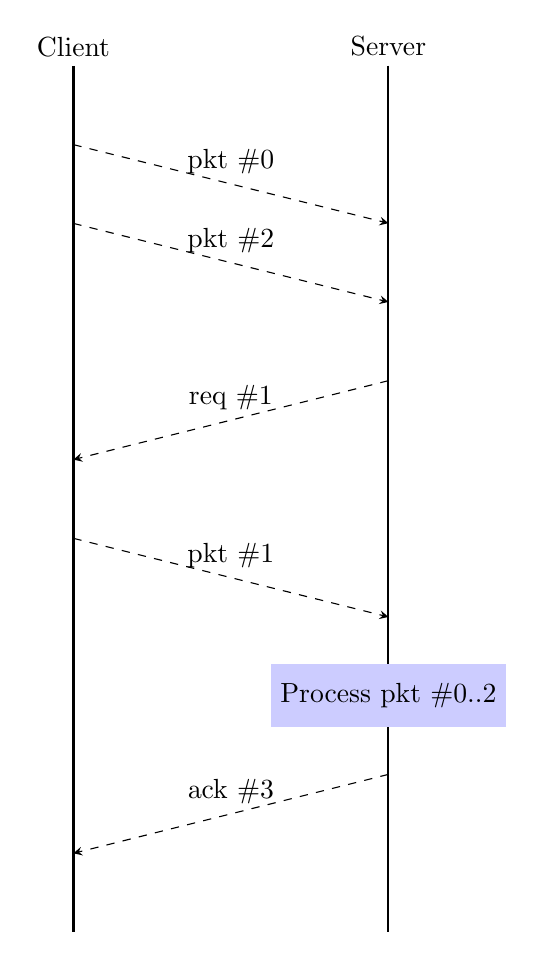
\begin{tikzpicture}[
    lifeline/.style={thick},
    message/.style={->, >=stealth, dashed},
    activation/.style={rectangle, fill=blue!20, minimum width=0.5cm, minimum height=0.8cm} ]

    \node[] (client) at (0,0) {Client};
    \node[] (server) at (4,0) {Server};

    \draw[lifeline] (client.south) -- ++(0,-11);
    \draw[lifeline] (server.south) -- ++(0,-11);

    \draw[message] ([yshift=-1cm] client.south) -- node[above] {pkt \#0} ([yshift=-2cm] server.south);
    \draw[message] ([yshift=-2cm] client.south) -- node[above] {pkt \#2} ([yshift=-3cm] server.south);
    \draw[message] ([yshift=-4cm] server.south) -- node[above] {req \#1} ([yshift=-5cm] client.south);
    \draw[message] ([yshift=-6cm] client.south) -- node[above] {pkt \#1} ([yshift=-7cm] server.south);
    \draw[message] ([yshift=-9cm] server.south) -- node[above] {ack \#3} ([yshift=-10cm] client.south);

    \node[activation] at ([yshift=-8cm] server.south) {Process pkt \#0..2};
 
\end{tikzpicture}
\end{center}

There are other design considerations. The server is allowed to send up to W
packets before getting an acknowledgement, this reduces latency perceived by the
user. The client also doesn't need to acknowledge all the packets, since the
server assumes once an acknowledgement of packet N is received, then all packets
prior to N have also been received.

\section{Design}

With the above description, we are now ready to provide a more formal
description for our design:

\begin{itemize}
    \item Client is the receiver that displays the video stream.
    \item Server is the sender that sends the video stream.
    \item Server always sends the packets in-order.
    \item Client may receive the packets out-of-order.
    \item Client may never receive some packet due to loss.
    \item Server can send up to W packets before an acknowledgement is received
    \item Packet sequence number is represented by a fixed number of bytes in
    the network header, the sequence number will eventually wrap around once it
    hits the maximum representable value. The maximum sequence number is
    represented as N-1. 
    \item Client puts a received packet in its receive buffer. Packets in the 
    receive buffer may be out-of-order due to network conditions.
    \item Client will remove the packets from the receive buffer once the
    sequence number of the received packets are contiguous. The client will also
    send an acknowledgement back to the Server with the most recently
    acknowledged sequence number.
    \item Data patckets are transported using unreliable channel due to
    bandwidth and latency requirement.
    \item Control packets are transported using reliable channel due to relaxed 
    and latency requirement. 
\end{itemize}

We are now ready to implement the \textit{Spec}. 

\section{Spec}

The following is the skeleton of the Spec: 
\newline

\begin{tla}
Init ==
    /\ network = {}
    /\ server_tx = 0
    /\ server_tx_limit = W
    /\ server_tx_ack = 0
    /\ client_rx = 0
    /\ client_buffer = {} 
    /\ lost = 0

Next == 
    \/ Send 
    \/ \E p \in network: 
        Receive(p)
    \/ ClientRetransmitRequest
    \/ ClientAcknowledgement
    \/ \E p \in network: 
        /\ p.dst = "client" 
        /\ Drop(p)
\end{tla}
\begin{tlatex}
\@x{ Init \.{\defeq}}%
\@x{\@s{16.4} \.{\land} network \.{=} \{ \}}%
\@x{\@s{16.4} \.{\land} server\_tx \.{=} 0}%
\@x{\@s{16.4} \.{\land} server\_tx\_limit \.{=} W}%
\@x{\@s{16.4} \.{\land} server\_tx\_ack \.{=} 0}%
\@x{\@s{16.4} \.{\land} client\_rx \.{=} 0}%
\@x{\@s{16.4} \.{\land} client\_buffer \.{=} \{ \}}%
\@x{\@s{16.4} \.{\land} lost \.{=} 0}%
\@pvspace{8.0pt}%
\@x{ Next \.{\defeq}}%
\@x{\@s{16.4} \.{\lor} Send}%
\@x{\@s{16.4} \.{\lor} \E\, p \.{\in} network \.{:}}%
\@x{\@s{20.5} Receive ( p )}%
\@x{\@s{16.4} \.{\lor} ClientRetransmitRequest}%
\@x{\@s{16.4} \.{\lor} ClientAcknowledgement}%
\@x{\@s{16.4} \.{\lor} \E\, p \.{\in} network \.{:}}%
\@x{\@s{20.5} \.{\land} p . dst \.{=}\@w{client}}%
\@x{\@s{20.5} \.{\land} Drop ( p )}%
\end{tlatex}
\newline

The server is represented by three variables: 
\begin{itemize}
    \item tx+1 represents the sequence number to be used in the next packet
    \item tx\_liimit represents the highest sequence number server can send
    without waiting for an acknowledgement
    \item tx\_ack represents the most recent acknowledged sequence number
\end{itemize}

The client is represented by two variables: 
\begin{itemize}
    \item client\_rx is the most recently acknowledged sequence number
    \item client\_buffer is the receive buffer holding all the packets waiting 
    to be re-ordered prior to being acknowleged 
\end{itemize}

The allowed actions include packet \textit{Receive}, which the existential
quantifier also has the side effect of re-ordering.
\textit{ClientRetransmitRequest} detects and sends retransmit request.
\textit{ClientAcknowledgement} sends acknowledgement. Finally, data packets may
be dropped.\newline

Before we start defining the actions, let us define some helper functions:\newline
\begin{tla}
MinS(s) == 
    CHOOSE x \in s: \A y \in s: x <= y

MaxS(s) == 
    CHOOSE x \in s: \A y \in s: x >= y

MaxIndex == 
    LET 
        upper == {x \in client_buffer : x > N - W}
        lower == {x \in client_buffer : x < W}
        maxv == IF upper # {} /\ lower # {} 
                THEN 
                    MaxS(lower)
                ELSE 
                    MaxS(client_buffer)
    IN 
        maxv

MinIndex == 
    LET 
        upper == {x \in client_buffer : x > N - W}
        lower == {x \in client_buffer : x < W}
        minv == IF upper # {} /\ lower # {} 
                THEN 
                    MinS(upper)
                ELSE 
                    MinS(client_buffer)
    IN 
        minv

Range == 
    IF MaxIndex >= MinIndex
    THEN
        MaxIndex - MinIndex + 1
    ELSE 
        MaxIndex + 1 + N - MinIndex
\end{tla}
\begin{tlatex}
\@x{ MinS ( s ) \.{\defeq}}%
\@x{ {\CHOOSE} x \.{\in} s \.{:} \A\, y \.{\in} s \.{:} x \.{\leq} y}%
\@pvspace{8.0pt}%
\@x{ MaxS ( s ) \.{\defeq}}%
\@x{ {\CHOOSE} x \.{\in} s \.{:} \A\, y \.{\in} s \.{:} x \.{\geq} y}%
\@pvspace{8.0pt}%
\@x{ MaxIndex \.{\defeq}}%
\@x{\@s{16.4} \.{\LET}}%
 \@x{\@s{32.8} upper \.{\defeq} \{ x \.{\in} client\_buffer \.{:} x \.{>} N
 \.{-} W \}}%
 \@x{\@s{32.8} lower \.{\defeq} \{ x \.{\in} client\_buffer \.{:} x \.{<} W
 \}}%
 \@x{\@s{32.8} maxv \.{\defeq} {\IF} upper \.{\neq} \{ \} \.{\land} lower
 \.{\neq} \{ \}}%
\@x{\@s{32.8} \.{\THEN}}%
\@x{\@s{49.19} MaxS ( lower )}%
\@x{\@s{32.8} \.{\ELSE}}%
\@x{\@s{49.19} MaxS ( client\_buffer )}%
\@x{\@s{16.4} \.{\IN}}%
\@x{\@s{32.8} maxv}%
\@pvspace{8.0pt}%
\@x{ MinIndex \.{\defeq}}%
\@x{\@s{16.4} \.{\LET}}%
 \@x{\@s{32.8} upper \.{\defeq} \{ x \.{\in} client\_buffer \.{:} x \.{>} N
 \.{-} W \}}%
 \@x{\@s{32.8} lower \.{\defeq} \{ x \.{\in} client\_buffer \.{:} x \.{<} W
 \}}%
 \@x{\@s{32.8} minv \.{\defeq} {\IF} upper \.{\neq} \{ \} \.{\land} lower
 \.{\neq} \{ \}}%
\@x{\@s{32.8} \.{\THEN}}%
\@x{\@s{49.19} MinS ( upper )}%
\@x{\@s{32.8} \.{\ELSE}}%
\@x{\@s{49.19} MinS ( client\_buffer )}%
\@x{\@s{16.4} \.{\IN}}%
\@x{\@s{32.8} minv}%
\@pvspace{8.0pt}%
\@x{ Range \.{\defeq}}%
\@x{\@s{16.4} {\IF} MaxIndex \.{\geq} MinIndex}%
\@x{\@s{16.4} \.{\THEN}}%
\@x{\@s{32.8} MaxIndex \.{-} MinIndex \.{+} 1}%
\@x{\@s{16.4} \.{\ELSE}}%
\@x{\@s{32.8} MaxIndex \.{+} 1 \.{+} N \.{-} MinIndex}%
\end{tlatex}
\newline

At any moment the system allows a window of packets to be unacknowledged. Both
the client and server are aware of the window size, represented by W. By looking
at packets in its receive buffer and its most acknowleged sequence number, the
client can determine which packets were lost. There's actually some nuisance 
to implement this.\newline

Since the system does not allow more than W unacknowledged packets, the client
can assume the window of packet in its receiver buffer must have sequence number
$s \in client\_rx ..client\_rx+W$. Since the sequence number has a ceiling, the
window of packets may wrap around the boundary. This introduces some
complication around determining the minimum and maximum in the window of packet.
The functions defined above calcluates the range, maximum and minimum value in
the window accounting for wraparound.\newline

Now we can look at how the client acknowledgement logic:\newline
\begin{tla}
MergeReady == 
    /\ client_buffer # {}
    /\ (client_rx + 1) % N = MinIndex       \* contiguous with previous ack
    /\ Range = Cardinality(client_buffer)   \* combined is contiguous 

ClientAcknowledgement == 
    /\ client_buffer # {}
    /\ MergeReady 
    /\ client_buffer' = {}
    /\ client_rx' = MaxIndex
    /\ network' = AddMessage([dst |-> "server",
                              type |-> "ack",
                              ack |-> MaxIndex], 
                                network)
    /\ UNCHANGED <<server_tx, server_tx_ack, server_tx_limit, lost>>
\end{tla}
\begin{tlatex}
\@x{ MergeReady \.{\defeq}}%
\@x{\@s{16.4} \.{\land} client\_buffer \.{\neq} \{ \}}%
 \@x{\@s{16.4} \.{\land} ( client\_rx \.{+} 1 ) \.{\%} N \.{=}
 MinIndex\@s{24.59}}%
\@y{%
  contiguous with previous ack
}%
\@xx{}%
\@x{\@s{16.4} \.{\land} Range \.{=} Cardinality ( client\_buffer )\@s{24.6}}%
\@y{%
  combined is contiguous 
}%
\@xx{}%
\@pvspace{8.0pt}%
\@x{ ClientAcknowledgement \.{\defeq}}%
\@x{\@s{16.4} \.{\land} client\_buffer \.{\neq} \{ \}}%
\@x{\@s{16.4} \.{\land} MergeReady}%
\@x{\@s{16.4} \.{\land} client\_buffer \.{'} \.{=} \{ \}}%
\@x{\@s{16.4} \.{\land} client\_rx \.{'} \.{=} MaxIndex}%
 \@x{\@s{16.4} \.{\land} network \.{'} \.{=} AddMessage ( [ dst
 \.{\mapsto}\@w{server} ,\, type \.{\mapsto}\@w{ack} ,\, ack \.{\mapsto}
 MaxIndex ] ,\, network )}%
 \@x{\@s{16.4} \.{\land} {\UNCHANGED} {\langle} server\_tx ,\, server\_tx\_ack
 ,\, server\_tx\_limit ,\, lost {\rangle}}%
\end{tlatex}
\newline

The client only acknowledges when it has a contiguous sequence of packets that
follows its most recently acknowledged packet. When MergeReady is true, the
client sends the acknowledgement back to the server.\newline

\begin{tla}
ClientReceive(pp) == 
    /\ network' = RemoveMessage(pp, network)
    /\ client_buffer' = client_buffer \cup {pp.seq}
    /\ UNCHANGED <<server_tx, client_rx, server_tx_ack, server_tx_limit, lost>>

Missing == 
    LET 
        full_seq == 
            IF MaxIndex >= client_rx+1 
            THEN 
                {x \in client_rx+1 .. MaxIndex : TRUE}
            ELSE 
                {x \in 0..MaxIndex : TRUE} \cup {x \in client_rx + 1..N-1 : TRUE}
        all_client_msgs == {m \in network: m.dst = "client"}
        all_client_seqs == {m.seq : m \in all_client_msgs}
        network_missing == full_seq \ all_client_seqs
        client_missing == full_seq \ client_buffer
        to_request == network_missing \intersect client_missing
    IN 
        to_request

ClientRetransmitRequest == 
    /\ ~MergeReady
    /\ client_buffer # {}
    /\ Missing # {}
    /\ network' = AddMessage([dst |-> "server", 
                              type |-> "retransmit",
                              seq |-> CHOOSE x \in Missing : TRUE],
                                network)
    /\ UNCHANGED <<server_tx, server_tx_limit, client_rx, client_buffer, server_tx_ack, lost>>
\end{tla}
\begin{tlatex}
\@x{ ClientReceive ( pp ) \.{\defeq}}%
\@x{\@s{16.4} \.{\land} network \.{'} \.{=} RemoveMessage ( pp ,\, network )}%
 \@x{\@s{16.4} \.{\land} client\_buffer \.{'} \.{=} client\_buffer \.{\cup} \{
 pp . seq \}}%
 \@x{\@s{16.4} \.{\land} {\UNCHANGED} {\langle} server\_tx ,\, client\_rx ,\,
 server\_tx\_ack ,\, server\_tx\_limit ,\, lost {\rangle}}%
\@pvspace{8.0pt}%
\@x{ Missing \.{\defeq}}%
\@x{\@s{16.4} \.{\LET}}%
\@x{\@s{32.8} full\_seq \.{\defeq}}%
\@x{\@s{49.19} {\IF} MaxIndex \.{\geq} client\_rx \.{+} 1}%
\@x{\@s{49.19} \.{\THEN}}%
 \@x{\@s{65.6} \{ x \.{\in} client\_rx \.{+} 1 \.{\dotdot} MaxIndex \.{:}
 {\TRUE} \}}%
\@x{\@s{49.19} \.{\ELSE}}%
 \@x{\@s{65.6} \{ x \.{\in} 0 \.{\dotdot} MaxIndex \.{:} {\TRUE} \} \.{\cup}
 \{ x \.{\in} client\_rx \.{+} 1 \.{\dotdot} N \.{-} 1 \.{:} {\TRUE} \}}%
 \@x{\@s{32.8} all\_client\_msgs \.{\defeq} \{ m \.{\in} network \.{:} m . dst
 \.{=}\@w{client} \}}%
 \@x{\@s{32.8} all\_client\_seqs \.{\defeq} \{ m . seq \.{:} m \.{\in}
 all\_client\_msgs \}}%
 \@x{\@s{32.8} network\_missing \.{\defeq} full\_seq \.{\,\backslash\,}
 all\_client\_seqs}%
 \@x{\@s{32.8} client\_missing \.{\defeq} full\_seq \.{\,\backslash\,}
 client\_buffer}%
 \@x{\@s{32.8} to\_request \.{\defeq} network\_missing \.{\cap}
 client\_missing}%
\@x{\@s{16.4} \.{\IN}}%
\@x{\@s{32.8} to\_request}%
\@pvspace{8.0pt}%
\@x{ ClientRetransmitRequest \.{\defeq}}%
\@x{\@s{16.4} \.{\land} {\lnot} MergeReady}%
\@x{\@s{16.4} \.{\land} client\_buffer \.{\neq} \{ \}}%
\@x{\@s{16.4} \.{\land} Missing \.{\neq} \{ \}}%
 \@x{\@s{16.4} \.{\land} network \.{'} \.{=} AddMessage ( [ dst
 \.{\mapsto}\@w{server} ,\,}%
\@x{\@s{16.4} type \.{\mapsto}\@w{retransmit} ,\,}%
 \@x{\@s{16.4} seq \.{\mapsto} {\CHOOSE} x \.{\in} Missing \.{:} {\TRUE} ]
 ,\,}%
\@x{\@s{24.59} network )}%
 \@x{\@s{16.4} \.{\land} {\UNCHANGED} {\langle} server\_tx ,\,
 server\_tx\_limit ,\, client\_rx ,\, client\_buffer ,\, server\_tx\_ack ,\,
 lost {\rangle}}%
\end{tlatex}
\newline

\textit{ClientReceive} moves the a packet from network into client receive
buffer. The only reason why this is done as a separate step is to make debugging
easier.\newline

\textit{Missing} returns a set of missing missing sequence number. This is done
by cross checking the client receive buffer and the outstanding network packet
targeting the client. In theory, the client doesn't know if a gap in its receive
buffer means the packet is lost or will arrive soon. Practically, the client
will assume a packet is lost after some configurable timeout and request a
retransmit.\newline

Let us take a look at server related definitions:\newline

\begin{tla}
RemoveStaleAck(ack, msgs) == 
    LET 
        acks == {(ack - k + N ) % N : k \in 1..W}
    IN 
        {m \in msgs : ~(m.dst = "server" /\ m.type = "ack" /\ m.ack \in acks)}

ServerReceive(pp) == 
    \/ /\ pp.type = "ack"
       /\ server_tx_ack' = pp.ack
       /\ server_tx_limit' = (pp.ack + W) % N
       /\ network' = RemoveStaleAck(pp.ack, RemoveMessage(pp, network))
       /\ UNCHANGED <<server_tx, client_rx, client_buffer, lost>>
    \/ /\ pp.type = "retransmit"
       /\ network' = AddMessage([dst |-> "client", seq |-> pp.seq], 
                                RemoveMessage(pp, network))
       /\ lost' = lost -1
       /\ UNCHANGED <<server_tx, server_tx_limit, client_rx, client_buffer, server_tx_ack>>
\end{tla}
\begin{tlatex}
\@x{ RemoveStaleAck ( ack ,\, msgs ) \.{\defeq}}%
\@x{\@s{16.4} \.{\LET}}%
 \@x{\@s{32.8} acks \.{\defeq} \{ ( ack \.{-} k \.{+} N ) \.{\%} N \.{:} k
 \.{\in} 1 \.{\dotdot} W \}}%
\@x{\@s{16.4} \.{\IN}}%
 \@x{\@s{32.8} \{ m \.{\in} msgs \.{:} {\lnot} ( m . dst \.{=}\@w{server}
 \.{\land} m . type \.{=}\@w{ack} \.{\land} m . ack \.{\in} acks ) \}}%
\@pvspace{8.0pt}%
\@x{ ServerReceive ( pp ) \.{\defeq}}%
\@x{\@s{16.4} \.{\lor} \.{\land} pp . type \.{=}\@w{ack}}%
\@x{\@s{16.4} \.{\land} server\_tx\_ack \.{'} \.{=} pp . ack}%
 \@x{\@s{16.4} \.{\land} server\_tx\_limit \.{'} \.{=} ( pp . ack \.{+} W )
 \.{\%} N}%
 \@x{\@s{16.4} \.{\land} network \.{'} \.{=} RemoveStaleAck ( pp . ack ,\,
 RemoveMessage ( pp ,\, network ) )}%
 \@x{\@s{16.4} \.{\land} {\UNCHANGED} {\langle} server\_tx ,\, client\_rx ,\,
 client\_buffer ,\, lost {\rangle}}%
\@x{\@s{16.4} \.{\lor} \.{\land} pp . type \.{=}\@w{retransmit}}%
 \@x{\@s{16.4} \.{\land} network \.{'} \.{=} AddMessage ( [ dst
 \.{\mapsto}\@w{client} ,\, seq \.{\mapsto} pp . seq ] ,\,}%
\@x{\@s{16.4} RemoveMessage ( pp ,\, network ) )}%
\@x{\@s{16.4} \.{\land} lost \.{'} \.{=} lost \.{-} 1}%
 \@x{\@s{16.4} \.{\land} {\UNCHANGED} {\langle} server\_tx ,\,
 server\_tx\_limit ,\, client\_rx ,\, client\_buffer ,\, server\_tx\_ack
 {\rangle}}%
\end{tlatex}
\newline

When the server receives an acknowledgement for sequence number K, it assumes
K-1 and prior were all received by the client. \textit{RemoveStaleAck} is an
model optimization to drop all acknowledgements with sequence number less than
K. Note that sequence number k, k-N, k-2*N, are all represented as k, and in
theory the client may not be able to differentiate betweeen them.  Practically,
N is sized large enough to represent a few seconds worth of data, so the system
can safely assume a sequence number k is for the most recent N packets.\newline

Upon receiving an acknowledgement from the client, the server bumps the
server\_tx\_limit allowing it to send more data. The server can also receive a 
retransmit request and send the requested data. \textit{lost} is configurable to
determine how many packets can be dropped at the same time.

\section{Model Reduction}

\subsection{Removing Stale Acknowlegement}

TODO: W * 2 < N
TODO: stale ack removal
TODO: describe network empty 
TODO: retransmit is assumed to be reliable, because making it unreliable doesn't make sense.

\section{Safety}

\section{Liveness}

Given the system may randomly drop packets, one possible liveness condition is
to verify packets of all sequence number are received by the client at some
point. This can be described as for all possible sequence number value k, k is
eventually exists in client receive buffer.\newline

\begin{tla}
Liveness == 
    \A i \in 0..N-1:
        client_buffer = {} ~> \E j \in client_buffer: i = j 
\end{tla}
\begin{tlatex}
\@x{ Liveness \.{\defeq}}%
\@x{\@s{16.4} \A\, i \.{\in} 0 \.{\dotdot} N \.{-} 1 \.{:}}%
 \@x{\@s{20.5} client\_buffer \.{=} \{ \} \.{\leadsto} \E\, j \.{\in}
 client\_buffer \.{:} i \.{=} j}%
\end{tlatex}
\newline






% \end{document}



\usetikzlibrary{arrows.meta} % For double arrows

\chapter{BitTorrent Protocol}

BitTorrent is a peer-to-peer file sharing protocol that allows users to 
distribute data in a decentralized fashion.\\

\begin{center}

\begin{tikzpicture}
    % Draw 5 "client" nodes in a bigger circle, labeled from 1 to 5
    \foreach \angle/\label in {0/1, 72/2, 144/3, 216/4, 288/5} {
        \node[draw, circle] (client\angle) at (\angle:5cm) {Client \label}; % Increased radius to 5cm
    }

    % Draw the "tracker" node in the center
    \node[draw, circle] (tracker) at (0,0) {Tracker};

    % Draw double-ended dotted lines from each client to the tracker
    \foreach \angle in {0, 72, 144, 216, 288} {
        \draw[Latex-Latex, dotted] (client\angle) -- (tracker);
    }

    % Draw single-line, double-ended arrows between all client nodes
    \foreach \source in {0, 72, 144, 216, 288} {
        \foreach \target in {72, 144, 216, 288, 0} {
            \ifnum\source<\target % Avoid duplicate and self-loops
                \draw[Latex-Latex] (client\source) -- (client\target);
            \fi
        }
    }
\end{tikzpicture}

\end{center}

% \begin{document}

\chapter{Raft Consensus Protocol}

Raft is a consensus algorithm that enables a cluster of nodes to agree on a
collective state even in the presence of failures. An application of Raft is
a database replication protocol. With a replication factor of 3 (eg. data is
replicated across 3 nodes) and a hard drive failure rate of 0.81\% per year, the
possibility of total failure where the entire replication group goes down is
$1-0.0081^3 = 99.9999\%$ uptime \cite{backblaze}.\\

This chapter implements only the leader election portion of the protocol to
limit the scope of the discussion. For a full description of the Raft
protocol, please refer to the original paper \cite{raft}.\\

\section{Design}

We will briefly describe Raft and its leadership election process below: 
\begin{itemize}
    \item A Raft cluster has N nodes, the cluster works collectively as a
    \textit{system} to offer some service
    \item Each node can be in one of three possible states: Follower, Candidate, Leader
    \item During normal operations, a cluster of N nodes has a single leader
    and N-1 followers
    \item The leader handles all the client interactions. Requests sent to followers will be 
    redirected to the leader
    \item The leader regularly sends a heartbeat to the follower, indicating its
    alive
    \item If a follower fails to receive a heartbeat from the leader after
    timeout, it will become a candidate, vote for itself, and campaign to be
    leader
    \item A candidate who collects the majority of the vote becomes the leader
    \item If multiple candidates are campaigning and a split vote happens,
    candidates will eventually declare an election timeout and start a new round of
    election
    \item The cluster can have multiple leaders due to unfavorable network conditions, 
    but the leaders must be on different terms 
    \item A newly elected leader will send a heartbeat to other nodes to establish 
    leadership 
    \item All requests and responses include the sender's term, allowing the
    receiver to react accordingly
\end{itemize}

The protocol also included a description of log synchronization, state
recovery, and more. Many details are omitted in this chapter to reduce modeling
costs. The N nodes in the cluster operate \textit{independently} following the
above heuristics. Hopefully, this highlights the complexity of verifying the
correctness of the protocol.\newline

The following illustrates the state diagram of one node in the cluster:\newline
\begin{center}
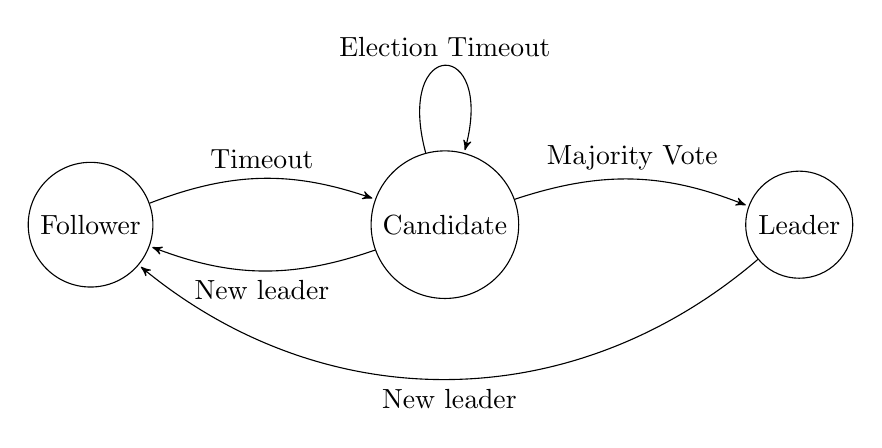
\begin{tikzpicture}[>=stealth',shorten >=1pt,auto,node distance=4.5cm]
  \node[state]  (f)                {Follower};
  \node[state]  (c) [right of=f]  {Candidate};
  \node[state]  (l) [right of=c]  {Leader};

  \path[->]          (f)  edge   [bend left=20]   node {Timeout} (c);
  \path[->]          (c)  edge   [bend left=20]   node {New leader} (f);

  \path[->]          (c)  edge   [bend left=20]   node {Majority Vote} (l);
  \path[->]          (l)  edge   [bend left=40]   node {New leader} (f);
  \path[->] (c) edge [loop above] node {Election Timeout} (c);

\end{tikzpicture}
\end{center}

\section{Spec}

The following implements the skeleton portion of the leader election
protocol:\newline

\begin{tla}
Init ==
    /\ state = [s \in Servers |-> "Follower"]
    /\ messages = {} 
    /\ voted_for = [s \in Servers |-> ""]
    /\ vote_granted = [s \in Servers |-> {}]
    /\ vote_requested = [s \in Servers |-> 0]
    /\ term = [s \in Servers |-> 0]

RequestVoteSet(i) == {
    [fSrc |-> i, fDst |-> s, fType |-> "RequestVoteReq", fTerm |-> term[i]] 
        : s \in Servers \ {i}
}

Campaign(i) == 
    /\ vote_requested[i] = 0
    /\ vote_requested' = [vote_requested EXCEPT ![i] = 1]
    /\ messages' = messages \cup RequestVoteSet(i) 
    /\ UNCHANGED <<state, term, vote_granted, voted_for>>

KeepAliveSet(i) == {
    [fSrc |-> i, fDst |-> s, fType |-> "AppendEntryReq", fTerm |-> term[i]] 
        : s \in Servers \ {i}
}

Leader(i) == 
    /\ state[i] = "Leader"
    /\ messages' = messages \cup KeepAliveSet(i) 
    /\ UNCHANGED <<state, voted_for, term, vote_granted, vote_requested>>

BecomeLeader(i) ==
    /\ Cardinality(vote_granted[i]) > Cardinality(Servers) \div 2
    /\ state' = [state EXCEPT ![i] = "Leader"]
    /\ UNCHANGED <<messages, voted_for, 
        term, vote_granted, vote_requested>>

Candidate(i) == 
    /\ state[i] = "Candidate"
    /\ \/ Campaign(i)
       \/ BecomeLeader(i)
       \/ Timeout(i)

Follower(i) == 
    /\ state[i] = "Follower"
    /\ Timeout(i)

Receive(msg) == 
    \/ /\ msg.fType = "AppendEntryReq"
       /\ AppendEntryReq(msg) 
    \/ /\ msg.fType = "AppendEntryResp"
       /\ AppendEntryResp(msg) 
    \/ /\ msg.fType = "RequestVoteReq"
       /\ RequestVoteReq(msg) 
    \/ /\ msg.fType = "RequestVoteResp"
       /\ RequestVoteResp(msg) 

Next == 
    \/ \E i \in Servers : 
          \/ Leader(i) 
          \/ Candidate(i)
          \/ Follower(i)
    \/ \E msg \in messages : Receive(msg)
\end{tla}
\begin{tlatex}
\@x{ Init \.{\defeq}}%
 \@x{\@s{16.4} \.{\land} state \.{=} [ s \.{\in} Servers
 \.{\mapsto}\@w{Follower} ]}%
\@x{\@s{16.4} \.{\land} messages \.{=} \{ \}}%
 \@x{\@s{16.4} \.{\land} voted\_for \.{=} [ s \.{\in} Servers \.{\mapsto}\@w{}
 ]}%
 \@x{\@s{16.4} \.{\land} vote\_granted \.{=} [ s \.{\in} Servers \.{\mapsto}
 \{ \} ]}%
 \@x{\@s{16.4} \.{\land} vote\_requested \.{=} [ s \.{\in} Servers \.{\mapsto}
 0 ]}%
\@x{\@s{16.4} \.{\land} term \.{=} [ s \.{\in} Servers \.{\mapsto} 0 ]}%
\@pvspace{8.0pt}%
\@x{ RequestVoteSet ( i ) \.{\defeq} \{}%
 \@x{\@s{16.4} [ fSrc \.{\mapsto} i ,\, fDst \.{\mapsto} s ,\, fType
 \.{\mapsto}\@w{RequestVoteReq} ,\, fTerm \.{\mapsto} term [ i ] ]}%
\@x{\@s{28.69} \.{:} s \.{\in} Servers \.{\,\backslash\,} \{ i \}}%
\@x{ \}}%
\@pvspace{8.0pt}%
\@x{ Campaign ( i ) \.{\defeq}}%
\@x{\@s{16.4} \.{\land} vote\_requested [ i ] \.{=} 0}%
 \@x{\@s{16.4} \.{\land} vote\_requested \.{'} \.{=} [ vote\_requested
 {\EXCEPT} {\bang} [ i ] \.{=} 1 ]}%
 \@x{\@s{16.4} \.{\land} messages \.{'} \.{=} messages \.{\cup} RequestVoteSet
 ( i )}%
 \@x{\@s{16.4} \.{\land} {\UNCHANGED} {\langle} state ,\, term ,\,
 vote\_granted ,\, voted\_for {\rangle}}%
\@pvspace{8.0pt}%
\@x{ KeepAliveSet ( i ) \.{\defeq} \{}%
 \@x{\@s{16.4} [ fSrc \.{\mapsto} i ,\, fDst \.{\mapsto} s ,\, fType
 \.{\mapsto}\@w{AppendEntryReq} ,\, fTerm \.{\mapsto} term [ i ] ]}%
\@x{\@s{28.69} \.{:} s \.{\in} Servers \.{\,\backslash\,} \{ i \}}%
\@x{ \}}%
\@pvspace{8.0pt}%
\@x{ Leader ( i ) \.{\defeq}}%
\@x{\@s{16.4} \.{\land} state [ i ] \.{=}\@w{Leader}}%
 \@x{\@s{16.4} \.{\land} messages \.{'} \.{=} messages \.{\cup} KeepAliveSet (
 i )}%
 \@x{\@s{16.4} \.{\land} {\UNCHANGED} {\langle} state ,\, voted\_for ,\, term
 ,\, vote\_granted ,\, vote\_requested {\rangle}}%
\@pvspace{8.0pt}%
\@x{ BecomeLeader ( i ) \.{\defeq}}%
 \@x{\@s{16.4} \.{\land} Cardinality ( vote\_granted [ i ] ) \.{>} Cardinality
 ( Servers ) \.{\div} 2}%
 \@x{\@s{16.4} \.{\land} state \.{'} \.{=} [ state {\EXCEPT} {\bang} [ i ]
 \.{=}\@w{Leader} ]}%
\@x{\@s{16.4} \.{\land} {\UNCHANGED} {\langle} messages ,\, voted\_for ,\,}%
\@x{\@s{20.5} term ,\, vote\_granted ,\, vote\_requested {\rangle}}%
\@pvspace{8.0pt}%
\@x{ Candidate ( i ) \.{\defeq}}%
\@x{\@s{16.4} \.{\land} state [ i ] \.{=}\@w{Candidate}}%
\@x{\@s{16.4} \.{\land} \.{\lor} Campaign ( i )}%
\@x{\@s{16.4} \.{\lor} BecomeLeader ( i )}%
\@x{\@s{16.4} \.{\lor} Timeout ( i )}%
\@pvspace{8.0pt}%
\@x{ Follower ( i ) \.{\defeq}}%
\@x{\@s{16.4} \.{\land} state [ i ] \.{=}\@w{Follower}}%
\@x{\@s{16.4} \.{\land} Timeout ( i )}%
\@pvspace{8.0pt}%
\@x{ Receive ( msg ) \.{\defeq}}%
\@x{\@s{16.4} \.{\lor} \.{\land} msg . fType \.{=}\@w{AppendEntryReq}}%
\@x{\@s{16.4} \.{\land} AppendEntryReq ( msg )}%
\@x{\@s{16.4} \.{\lor} \.{\land} msg . fType \.{=}\@w{AppendEntryResp}}%
\@x{\@s{16.4} \.{\land} AppendEntryResp ( msg )}%
\@x{\@s{16.4} \.{\lor} \.{\land} msg . fType \.{=}\@w{RequestVoteReq}}%
\@x{\@s{16.4} \.{\land} RequestVoteReq ( msg )}%
\@x{\@s{16.4} \.{\lor} \.{\land} msg . fType \.{=}\@w{RequestVoteResp}}%
\@x{\@s{16.4} \.{\land} RequestVoteResp ( msg )}%
\@pvspace{8.0pt}%
\@x{ Next \.{\defeq}}%
\@x{\@s{16.4} \.{\lor} \E\, i \.{\in} Servers \.{:}}%
\@x{\@s{16.4} \.{\lor} Leader ( i )}%
\@x{\@s{16.4} \.{\lor} Candidate ( i )}%
\@x{\@s{16.4} \.{\lor} Follower ( i )}%
\@x{\@s{16.4} \.{\lor} \E\, msg \.{\in} messages \.{:} Receive ( msg )}%
\end{tlatex}

\begin{itemize}
    \item \textit{Next} either picks a server to make progress, or picks a
    message in the message pool to process. Message processing is done by
    \textit{Receive}, handling is state agnostic
    \item \textit{message} is defined to be a set that holds a collection of functions, where 
    each function is a message with source, destination, type, and more specified
    \item \textit{voted\_for} tracks who a given node previously voted for.
    This prevents a node from voting more than once
    \item \textit{vote\_granted} tracks how many votes a candidate has received
    \item \textit{vote\_requested} tracks if a node has already issued a request
    vote to its peers
    \item \textit{Follower} either Receive or Timeout and campaign to be a leader
    \item \textit{Candidate} campaigns to be a leader, and becomes one if it has
    enough vote. Failing to collect enough votes, \textit{Candidate} start a new
    election on a new term. It can also receive a request with a higher term and
    transition to be a \textit{Follower}.
    \item \textit{Leader} will establish its leadership by sending
    \textit{AppepndEntryReq} to all its peers
\end{itemize}

 \textit{Spec} implements four messages AppendEntry request/response, RequestVote
request/response. Handling for all messages is similar in structure. In
this chapter, we will look at \textit{RequestVoteReq} only. Readers are
encouraged to check the remaining definition as an exercise:\newline

\begin{tla}
RequestVoteReq(msg) == 
    LET 
        i == msg.fDst
        j == msg.fSrc
        type == msg.fType
        t == msg.fTerm
    IN 
        \* haven't voted, or whom we voted re-requested
        \/ /\ t = term[i]
           /\ \/ voted_for[i] = j 
              \/ voted_for[i] = ""
           /\ voted_for' = [voted_for EXCEPT ![i] = j]
           /\ messages' = AddMessage([fSrc |-> i, 
                                        fDst |-> j, 
                                        fType |-> "RequestVoteResp",
                                        fTerm |-> t, 
                                        fSuccess |-> 1],
                                        RemoveMessage(msg, messages))
           /\ UNCHANGED <<state, term, vote_granted, 
                vote_requested, establish_leadership >>
        \* already voted for someone else
        \/ /\ t = term[i]
           /\ voted_for[i] # j 
           /\ voted_for[i] # ""
           /\ messages' = AddMessage([fSrc |-> i, 
                                        fDst |-> j, 
                                        fType |-> "RequestVoteResp",
                                        fTerm |-> t, 
                                        fSuccess |-> 0],
                                        RemoveMessage(msg, messages))
            /\ UNCHANGED <<state, voted_for, term, 
                vote_granted, vote_requested, establish_leadership>>
        \/  /\ t < term[i]
            /\ messages' = AddMessage([fSrc |-> i, 
                                        fDst |-> j, 
                                        fType |-> "RequestVoteResp",
                                        fTerm |-> term[i], 
                                        fSuccess |-> 0],
                                        RemoveMessage(msg, messages))
            /\ UNCHANGED <<state, voted_for, term, 
                vote_granted, vote_requested, establish_leadership>>
        \* revert to follower
        \/  /\ t > term[i]
            /\ state' = [state EXCEPT ![i] = "Follower"]
            /\ term' = [term EXCEPT ![i] = t]
            /\ voted_for' = [voted_for EXCEPT ![i] = j]
            /\ vote_granted' = [vote_granted EXCEPT ![i] = {}]
            /\ vote_requested' = [vote_requested EXCEPT ![i] = 0]
            /\ establish_leadership' = [establish_leadership EXCEPT ![i] = 0]
            /\ messages' = AddMessage([fSrc |-> i, 
                                        fDst |-> j, 
                                        fType |-> "RequestVoteResp",
                                        fTerm |-> t, 
                                        fSuccess |-> 1],
                                        RemoveMessage(msg, messages))
\end{tla}
\begin{tlatex}
\@x{ RequestVoteReq ( msg ) \.{\defeq}}%
\@x{\@s{16.4} \.{\LET}}%
\@x{\@s{32.8} i \.{\defeq} msg . fDst}%
\@x{\@s{32.8} j \.{\defeq} msg . fSrc}%
\@x{\@s{32.8} type \.{\defeq} msg . fType}%
\@x{\@s{32.8} t \.{\defeq} msg . fTerm}%
\@x{\@s{16.4} \.{\IN}}%
\@x{\@s{32.8}}%
\@y{%
  haven't voted, or whom we voted re-requested
}%
\@xx{}%
\@x{\@s{32.8} \.{\lor} \.{\land} t \.{=} term [ i ]}%
\@x{\@s{32.8} \.{\land} \.{\lor} voted\_for [ i ] \.{=} j}%
\@x{\@s{32.8} \.{\lor} voted\_for [ i ] \.{=}\@w{}}%
 \@x{\@s{32.8} \.{\land} voted\_for \.{'} \.{=} [ voted\_for {\EXCEPT} {\bang}
 [ i ] \.{=} j ]}%
 \@x{\@s{32.8} \.{\land} messages \.{'} \.{=} AddMessage ( [ fSrc \.{\mapsto}
 i ,\,}%
\@x{\@s{41.0} fDst \.{\mapsto} j ,\,}%
\@x{\@s{41.0} fType \.{\mapsto}\@w{RequestVoteResp} ,\,}%
\@x{\@s{41.0} fTerm \.{\mapsto} t ,\,}%
\@x{\@s{41.0} fSuccess \.{\mapsto} 1 ] ,\,}%
\@x{\@s{41.0} RemoveMessage ( msg ,\, messages ) )}%
 \@x{\@s{32.8} \.{\land} {\UNCHANGED} {\langle} state ,\, term ,\,
 vote\_granted ,\,}%
\@x{\@s{41.0} vote\_requested ,\, establish\_leadership {\rangle}}%
\@x{\@s{32.8}}%
\@y{%
  already voted for someone else
}%
\@xx{}%
\@x{\@s{32.8} \.{\lor} \.{\land} t \.{=} term [ i ]}%
\@x{\@s{32.8} \.{\land} voted\_for [ i ] \.{\neq} j}%
\@x{\@s{32.8} \.{\land} voted\_for [ i ] \.{\neq}\@w{}}%
 \@x{\@s{32.8} \.{\land} messages \.{'} \.{=} AddMessage ( [ fSrc \.{\mapsto}
 i ,\,}%
\@x{\@s{41.0} fDst \.{\mapsto} j ,\,}%
\@x{\@s{41.0} fType \.{\mapsto}\@w{RequestVoteResp} ,\,}%
\@x{\@s{41.0} fTerm \.{\mapsto} t ,\,}%
\@x{\@s{41.0} fSuccess \.{\mapsto} 0 ] ,\,}%
\@x{\@s{41.0} RemoveMessage ( msg ,\, messages ) )}%
 \@x{\@s{36.89} \.{\land} {\UNCHANGED} {\langle} state ,\, voted\_for ,\, term
 ,\,}%
 \@x{\@s{40.99} vote\_granted ,\, vote\_requested ,\, establish\_leadership
 {\rangle}}%
\@x{\@s{32.8} \.{\lor}\@s{4.1} \.{\land} t \.{<} term [ i ]}%
 \@x{\@s{36.89} \.{\land} messages \.{'} \.{=} AddMessage ( [ fSrc \.{\mapsto}
 i ,\,}%
\@x{\@s{40.99} fDst \.{\mapsto} j ,\,}%
\@x{\@s{40.99} fType \.{\mapsto}\@w{RequestVoteResp} ,\,}%
\@x{\@s{40.99} fTerm \.{\mapsto} term [ i ] ,\,}%
\@x{\@s{40.99} fSuccess \.{\mapsto} 0 ] ,\,}%
\@x{\@s{40.99} RemoveMessage ( msg ,\, messages ) )}%
 \@x{\@s{36.89} \.{\land} {\UNCHANGED} {\langle} state ,\, voted\_for ,\, term
 ,\,}%
 \@x{\@s{40.99} vote\_granted ,\, vote\_requested ,\, establish\_leadership
 {\rangle}}%
\@x{\@s{32.8}}%
\@y{%
  revert to follower
}%
\@xx{}%
\@x{\@s{32.8} \.{\lor}\@s{4.1} \.{\land} t \.{>} term [ i ]}%
 \@x{\@s{36.89} \.{\land} state \.{'} \.{=} [ state {\EXCEPT} {\bang} [ i ]
 \.{=}\@w{Follower} ]}%
 \@x{\@s{36.89} \.{\land} term \.{'} \.{=} [ term {\EXCEPT} {\bang} [ i ]
 \.{=} t ]}%
 \@x{\@s{36.89} \.{\land} voted\_for \.{'} \.{=} [ voted\_for {\EXCEPT}
 {\bang} [ i ] \.{=} j ]}%
 \@x{\@s{36.89} \.{\land} vote\_granted \.{'} \.{=} [ vote\_granted {\EXCEPT}
 {\bang} [ i ] \.{=} \{ \} ]}%
 \@x{\@s{36.89} \.{\land} vote\_requested \.{'} \.{=} [ vote\_requested
 {\EXCEPT} {\bang} [ i ] \.{=} 0 ]}%
 \@x{\@s{36.89} \.{\land} establish\_leadership \.{'} \.{=} [
 establish\_leadership {\EXCEPT} {\bang} [ i ] \.{=} 0 ]}%
 \@x{\@s{36.89} \.{\land} messages \.{'} \.{=} AddMessage ( [ fSrc \.{\mapsto}
 i ,\,}%
\@x{\@s{40.99} fDst \.{\mapsto} j ,\,}%
\@x{\@s{40.99} fType \.{\mapsto}\@w{RequestVoteResp} ,\,}%
\@x{\@s{40.99} fTerm \.{\mapsto} t ,\,}%
\@x{\@s{40.99} fSuccess \.{\mapsto} 1 ] ,\,}%
\@x{\@s{40.99} RemoveMessage ( msg ,\, messages ) )}%
\end{tlatex}
\newline

The handling is split into three cases: 
\begin{itemize}
    \item If the received request is on a higher term, the processing node grants a vote and becomes a Follower
    \item If the received request is on a lower term, the processing node ignores the request
    \item If the received request is on the same term, the processing node only grants
    vote if it hasn't voted, or has voted for the same requester prior 
\end{itemize}

\section{Refinement}

The model checker will run \textit{Spec} as defined, but is unlikely to be
completed in a reasonable amount of time due to exponential state growth. We
need to simplify the model, and careful consideration must go into finding the
right balance between maximizing model correctness and minimizing model checker
runtime.\newline

The main strategy is to \textit{bound} the state graph. The following describes
a set of optimization implemented for this example.

\subsection{Modeling Messages as a Set}

In the original Raft TLA+ Spec \cite{raft_tla}, messages are modeled as an
\textit{unordered map} to track the count of each message. It is possible for a
sender to repeatedly send the same message (eg. keepalive), and grow the 
message count in an unbounded fashion.\newline

\textit{messages} in this example has been implemented as a set, which
effectively limits the message instance count to one. It is still possible for
messages to grow unboundedly because of the monotonically increasing term value.
Further changes are described below.

\subsection{Limit Term Divergence} 

It is possible for a node to \textit{never} make progress. Such a case can occur
when a node is partitioned off while the rest of the cluster elects a new leader
and moves onto newer terms. Many of the interesting behaviors of Raft are how it
addresses these cases. In a cluster of nodes with mixed terms, the nodes with
older terms will eventually converge onto newer terms when they are contacted by
a new leader. This converging behavior will happen whether the stale node is
either 1 or N terms away from the current leader, and the former is much less
costly to simulate than the latter because of the reduced number of states.\newline

We can include \textit{LimitDivergence} as a conjunction in
\textit{Timeout}:\newline
\begin{tla}
LimitDivergence(i) == 
    LET 
        values == {term[s] : s \in Servers}
        max_v == CHOOSE x \in values : \A y \in values : x >= y
        min_v == CHOOSE x \in values : \A y \in values : x <= y
    IN 
        \/ /\ term[i] # max_v
        \/ /\ term[i] = max_v 
           /\ term[i] - min_v < MaxDiff

Timeout(i) == 
    /\ LimitDivergence(i)
    /\ state' = [state EXCEPT ![i] = "Candidate"]
    /\ voted_for' = [voted_for EXCEPT ![i] = i]             \* voted for myself
    /\ vote_granted' = [vote_granted EXCEPT ![i] = {i}]
    /\ vote_requested' = [vote_requested EXCEPT ![i] = 0]
    /\ term' = [term EXCEPT ![i] = @ + 1]                   \* bump term
    /\ establish_leadership' = [establish_leadership EXCEPT ![i] = 0]
    /\ UNCHANGED <<messages>>
    \* /\ PrintT(state')
\end{tla}
\begin{tlatex}
\@x{ LimitDivergence ( i ) \.{\defeq}}%
\@x{\@s{16.4} \.{\LET}}%
\@x{\@s{32.8} values \.{\defeq} \{ term [ s ] \.{:} s \.{\in} Servers \}}%
 \@x{\@s{32.8} max\_v \.{\defeq} {\CHOOSE} x \.{\in} values \.{:} \A\, y
 \.{\in} values \.{:} x \.{\geq} y}%
 \@x{\@s{32.8} min\_v \.{\defeq} {\CHOOSE} x \.{\in} values \.{:} \A\, y
 \.{\in} values \.{:} x \.{\leq} y}%
\@x{\@s{16.4} \.{\IN}}%
\@x{\@s{32.8} \.{\lor} \.{\land} term [ i ] \.{\neq} max\_v}%
\@x{\@s{32.8} \.{\lor} \.{\land} term [ i ] \.{=} max\_v}%
\@x{\@s{32.8} \.{\land} term [ i ] \.{-} min\_v \.{<} MaxDiff}%
\@pvspace{8.0pt}%
\@x{ Timeout ( i ) \.{\defeq}}%
\@x{\@s{16.4} \.{\land} LimitDivergence ( i )}%
 \@x{\@s{16.4} \.{\land} state \.{'} \.{=} [ state {\EXCEPT} {\bang} [ i ]
 \.{=}\@w{Candidate} ]}%
 \@x{\@s{16.4} \.{\land} voted\_for \.{'} \.{=} [ voted\_for {\EXCEPT} {\bang}
 [ i ] \.{=} i ]\@s{49.19}}%
\@y{%
  voted for myself
}%
\@xx{}%
 \@x{\@s{16.4} \.{\land} vote\_granted \.{'} \.{=} [ vote\_granted {\EXCEPT}
 {\bang} [ i ] \.{=} \{ i \} ]}%
 \@x{\@s{16.4} \.{\land} vote\_requested \.{'} \.{=} [ vote\_requested
 {\EXCEPT} {\bang} [ i ] \.{=} 0 ]}%
 \@x{\@s{16.4} \.{\land} term \.{'} \.{=} [ term {\EXCEPT} {\bang} [ i ] \.{=}
 @ \.{+} 1 ]\@s{49.19}}%
\@y{%
  bump term
}%
\@xx{}%
 \@x{\@s{16.4} \.{\land} establish\_leadership \.{'} \.{=} [
 establish\_leadership {\EXCEPT} {\bang} [ i ] \.{=} 0 ]}%
\@x{\@s{16.4} \.{\land} {\UNCHANGED} {\langle} messages {\rangle}}%
\@x{\@s{16.4}}%
\@y{%
  /\ PrintT(state')
}%
\@xx{}%
\end{tlatex}

\subsection{Normalize Cluster Term}

However, \textit{term} can grow unbounded. A monotonically increasing counter is
what many consensus protocol rely on to represent the latest reality. We want to
\textit{normalize} the range of terms in the cluster so the minimum value resets
back to 0 to bound the state graph. This is a trick described in \cite{finite}.
\\

\begin{tla}
Normalize == 
    LET 
        values == {term[s] : s \in Servers}
        max_v == CHOOSE x \in values : \A y \in values : x >= y
        min_v == CHOOSE x \in values : \A y \in values : x <= y
    IN 
        /\ max_v = MaxTerm
        /\ term' = [s \in Servers |-> term[s] - min_v]
        /\ messages' = {}
        /\ UNCHANGED <<state, voted_for, 
            vote_granted, vote_requested, establish_leadership>>

Next == 
    \/ /\ \A i \in Servers : term[i] # MaxTerm 
       /\ \/ \E i \in Servers : 
                \/ Leader(i) 
                \/ Candidate(i)
                \/ Follower(i)
          \/ \E msg \in messages : Receive(msg)
    \/ /\ \E i \in Servers: term[i] = MaxTerm 
       /\ Normalize
\end{tla}
\begin{tlatex}
\@x{ Normalize \.{\defeq}}%
\@x{\@s{16.4} \.{\LET}}%
\@x{\@s{32.8} values \.{\defeq} \{ term [ s ] \.{:} s \.{\in} Servers \}}%
 \@x{\@s{32.8} max\_v \.{\defeq} {\CHOOSE} x \.{\in} values \.{:} \A\, y
 \.{\in} values \.{:} x \.{\geq} y}%
 \@x{\@s{32.8} min\_v \.{\defeq} {\CHOOSE} x \.{\in} values \.{:} \A\, y
 \.{\in} values \.{:} x \.{\leq} y}%
\@x{\@s{16.4} \.{\IN}}%
\@x{\@s{32.8} \.{\land} max\_v \.{=} MaxTerm}%
 \@x{\@s{32.8} \.{\land} term \.{'} \.{=} [ s \.{\in} Servers \.{\mapsto} term
 [ s ] \.{-} min\_v ]}%
\@x{\@s{32.8} \.{\land} messages \.{'} \.{=} \{ \}}%
\@x{\@s{32.8} \.{\land} {\UNCHANGED} {\langle} state ,\, voted\_for ,\,}%
 \@x{\@s{36.89} vote\_granted ,\, vote\_requested ,\, establish\_leadership
 {\rangle}}%
\@pvspace{8.0pt}%
\@x{ Next \.{\defeq}}%
 \@x{\@s{16.4} \.{\lor} \.{\land} \A\, i \.{\in} Servers \.{:} term [ i ]
 \.{\neq} MaxTerm}%
\@x{\@s{16.4} \.{\land} \.{\lor} \E\, i \.{\in} Servers \.{:}}%
\@x{\@s{16.4} \.{\lor} Leader ( i )}%
\@x{\@s{16.4} \.{\lor} Candidate ( i )}%
\@x{\@s{16.4} \.{\lor} Follower ( i )}%
\@x{\@s{16.4} \.{\lor} \E\, msg \.{\in} messages \.{:} Receive ( msg )}%
 \@x{\@s{16.4} \.{\lor} \.{\land} \E\, i \.{\in} Servers \.{:} term [ i ]
 \.{=} MaxTerm}%
\@x{\@s{16.4} \.{\land} Normalize}%
\end{tlatex}
\newline

The implementation ensures only the state machine only moves forward when none
of the nodes is on \textit{MaxTerm}. If any of the nodes are on \textit{MaxTerm},
the cluster terms are normalized.\newline

Another caveat here is in the initial implementation I didn't update messages.
This led to liveness property violation as the messages had terms disagreeing
with the system state. To simplify \textit{Spec} I simply cleared all messages. This 
indirectly verifies a portion of the packet loss handling in \textit{Spec} as well.

\subsection{Sending Request as a Batch}

The send requests were initially implemented using the existential quantifier. 
This introduces many interleaving states. This was replaced with a universal
quantifier so the set of messages is only sent once. The implementation no
longer tracks if the responses were received since \textit{Spec} should handle
packet loss scenarios as well.\\

\begin{tla}
RequestVoteSet(i) == {
    [fSrc |-> i, fDst |-> s, fType |-> "RequestVoteReq", fTerm |-> term[i]] 
        : s \in Servers \ {i}
}

Campaign(i) == 
    /\ vote_requested[i] = 0
    /\ vote_requested' = [vote_requested EXCEPT ![i] = 1]
    /\ messages' = messages \cup RequestVoteSet(i) 
    /\ UNCHANGED <<state, term, vote_granted, 
        voted_for, establish_leadership>>

KeepAliveSet(i) == {
    [fSrc |-> i, fDst |-> s, fType |-> "AppendEntryReq", fTerm |-> term[i]] 
        : s \in Servers \ {i}
}

Leader(i) == 
    /\ state[i] = "Leader"
    /\ establish_leadership[i] = 0
    /\ establish_leadership' = [establish_leadership EXCEPT ![i] = 1]
    /\ messages' = messages \cup KeepAliveSet(i) 
    /\ UNCHANGED <<state, voted_for, term, vote_granted, vote_requested>>
\end{tla}
\begin{tlatex}
\@x{ RequestVoteSet ( i ) \.{\defeq} \{}%
 \@x{\@s{16.4} [ fSrc \.{\mapsto} i ,\, fDst \.{\mapsto} s ,\, fType
 \.{\mapsto}\@w{RequestVoteReq} ,\, fTerm \.{\mapsto} term [ i ] ]}%
\@x{\@s{28.69} \.{:} s \.{\in} Servers \.{\,\backslash\,} \{ i \}}%
\@x{ \}}%
\@pvspace{8.0pt}%
\@x{ Campaign ( i ) \.{\defeq}}%
\@x{\@s{16.4} \.{\land} vote\_requested [ i ] \.{=} 0}%
 \@x{\@s{16.4} \.{\land} vote\_requested \.{'} \.{=} [ vote\_requested
 {\EXCEPT} {\bang} [ i ] \.{=} 1 ]}%
 \@x{\@s{16.4} \.{\land} messages \.{'} \.{=} messages \.{\cup} RequestVoteSet
 ( i )}%
 \@x{\@s{16.4} \.{\land} {\UNCHANGED} {\langle} state ,\, term ,\,
 vote\_granted ,\,}%
\@x{\@s{20.5} voted\_for ,\, establish\_leadership {\rangle}}%
\@pvspace{8.0pt}%
\@x{ KeepAliveSet ( i ) \.{\defeq} \{}%
 \@x{\@s{16.4} [ fSrc \.{\mapsto} i ,\, fDst \.{\mapsto} s ,\, fType
 \.{\mapsto}\@w{AppendEntryReq} ,\, fTerm \.{\mapsto} term [ i ] ]}%
\@x{\@s{28.69} \.{:} s \.{\in} Servers \.{\,\backslash\,} \{ i \}}%
\@x{ \}}%
\@pvspace{8.0pt}%
\@x{ Leader ( i ) \.{\defeq}}%
\@x{\@s{16.4} \.{\land} state [ i ] \.{=}\@w{Leader}}%
\@x{\@s{16.4} \.{\land} establish\_leadership [ i ] \.{=} 0}%
 \@x{\@s{16.4} \.{\land} establish\_leadership \.{'} \.{=} [
 establish\_leadership {\EXCEPT} {\bang} [ i ] \.{=} 1 ]}%
 \@x{\@s{16.4} \.{\land} messages \.{'} \.{=} messages \.{\cup} KeepAliveSet (
 i )}%
 \@x{\@s{16.4} \.{\land} {\UNCHANGED} {\langle} state ,\, voted\_for ,\, term
 ,\, vote\_granted ,\, vote\_requested {\rangle}}%
\end{tlatex}

\subsection{Prune Messages with Stale Terms}

When a node's term advances, all messages targeted to this node with older terms
are discarded. Keeping messages with stale terms allows the model checker to 
verify the node correctly discards them, but can exponentially grow the state
machine. To simplify the model, we can prune stale messages as we add a new 
message: \newline

\begin{tla}
AddMessage(to_add, msgs) == 
    LET 
        pruned == {msg \in msgs : 
                    ~(msg.fDst = to_add.fDst /\ msg.fTerm < to_add.fTerm)}
    IN
        pruned \cup {to_add}

RemoveMessage(to_remove, msgs) ==
\end{tla}
\begin{tlatex}
\@x{ AddMessage ( to\_add ,\, msgs ) \.{\defeq}}%
\@x{\@s{16.4} \.{\LET}}%
\@x{\@s{32.8} pruned \.{\defeq} \{ msg \.{\in} msgs \.{:}}%
 \@x{\@s{36.89} {\lnot} ( msg . fDst \.{=} to\_add . fDst \.{\land} msg .
 fTerm \.{<} to\_add . fTerm ) \}}%
\@x{\@s{16.4} \.{\IN}}%
\@x{\@s{32.8} pruned \.{\cup} \{ to\_add \}}%
\@pvspace{8.0pt}%
\@x{ RemoveMessage ( to\_remove ,\, msgs ) \.{\defeq}}%
\end{tlatex}

\subsection{Enable Symmetry}

Since the behavior is symmetric between nodes, we can enable symmetry to speed
up model checker runtime:\newline

\begin{tla}
Perms == Permutations(Servers)
\end{tla}
\begin{tlatex}
\@x{ Perms \.{\defeq} Permutations ( Servers )}%
\end{tlatex}

\section{Safety}

One of the goals of the protocol is to ensure the cluster only has one leader.
The clusters can have multiple leaders due to unfavorable network connections. For example, a leader node is partitioned off and a new
leader is elected. However, even when the cluster has multiple leaders, they
\textit{must} be on different terms. The leader with the highest term is
effectively the \textit{true leader}. This invariant can be implemented like
so:\newline

\begin{tla}
LeaderUniqueTerm ==
    \A s1, s2 \in Servers :
        (/\state[s1] = "Leader" 
         /\ state[s2] = "Leader" 
         /\ s1 /= s2)   
            => (term[s1] # term[s2])
\end{tla}
\begin{tlatex}
\@x{ LeaderUniqueTerm \.{\defeq}}%
\@x{\@s{16.4} \A\, s1 ,\, s2 \.{\in} Servers \.{:}}%
\@x{\@s{20.5} ( \.{\land} state [ s1 ] \.{=}\@w{Leader}}%
\@x{\@s{24.6} \.{\land} state [ s2 ] \.{=}\@w{Leader}}%
\@x{\@s{24.6} \.{\land} s1 \.{\neq} s2 )}%
\@x{\@s{24.6} \.{\implies} ( term [ s1 ] \.{\neq} term [ s2 ] )}%
\end{tlatex}
\newline

For every pair of nodes, they cannot both be Leaders and have the same
term.

\section{Liveness}

In any failure recovery scenario, the nodes in the cluster converge to a higher
term value either voluntarily or involuntarily. For example: 
\begin{itemize}
    \item A node timed out and started a new election on a new term 
    \item A partitioned follower receives a heartbeat from a new leader on a new term
    \item A candidate receiving a request vote from another candidate on a higher term
\end{itemize}

In any case, a node's term number always increases. This can be described as below:\newline
\begin{tla}
Converge ==
    \A s \in Servers:
        term[s] = 0 ~> term[s] = MaxTerm - MaxDiff
\end{tla}
\begin{tlatex}
\@x{ Converge \.{\defeq}}%
\@x{\@s{16.4} \A\, s \.{\in} Servers \.{:}}%
 \@x{\@s{20.5} term [ s ] \.{=} 0 \.{\leadsto} term [ s ] \.{=} MaxTerm \.{-}
 MaxDiff}%
\end{tlatex}
\newline

Instead of \textit{MaxTerm}, we use \textit{MaxTerm-MaxDiff} to ensure the
liveness property is always upheld even after \textit{Normalization}. However,
running  \textit{Spec} against TLC now will encounter a set of stuttering issues. We
also need to update the fairness description to ensure all possible actions are
called when the enabling conditions are \textit{eventually always} true:\newline

\begin{tla}
Liveness == 
    /\ \A i \in Servers : 
        /\ WF_vars(Leader(i))
        /\ WF_vars(Candidate(i))
        /\ WF_vars(Follower(i))
    /\ WF_vars(\E msg \in messages : Receive(msg))
\end{tla}
\begin{tlatex}
\@x{ Liveness \.{\defeq}}%
\@x{\@s{16.4} \.{\land} \A\, i \.{\in} Servers \.{:}}%
\@x{\@s{20.5} \.{\land} {\WF}_{ vars} ( Leader ( i ) )}%
\@x{\@s{20.5} \.{\land} {\WF}_{ vars} ( Candidate ( i ) )}%
\@x{\@s{20.5} \.{\land} {\WF}_{ vars} ( Follower ( i ) )}%
 \@x{\@s{16.4} \.{\land} {\WF}_{ vars} ( \E\, msg \.{\in} messages \.{:}
 Receive ( msg ) )}%
\end{tlatex}

% \end{document}


\part{Examples with PlusCal}

PlusCal is a C-like syntax that allows designer to describe their specification
using a pseudo programming language. An use case for PlusCal is to specify
lockless or wait-free data structures.\\

It is possible to express concurrent data structures in TLA+ native notation. To
express a function that can be concurrently executed, the specification needs to
use a PC-like variable to track the statement a context is currently executing.
This is fairly tedious (and possibly error-prone), making PlusCal a more organic
tool to express these designs. 

CONSTANT defaultInitValue = defaultInitValue
\* Add statements after this line.

SPECIFICATION Spec
\* INVARIANTS TypeOK NotSolved

CONSTANTS 
    N = 8
    M = 2
    Reader = 2
    Writer = 1

INVARIANTS 
    \* Inv_UniqueReaderPointers
    \* Inv_ReadingVsReady
    \* Inv_NonZeroCount
    \* Inv_UniqueReader
    \* Inv_DataValidity
    \* Inv_BufferSlotLifecycle
    \* Inv_ProducerConsumerSeparation
    Inv_Basics
    \* Inv_DataValidity2


% \begin{document}

\chapter{SPMC Lockless Queue}

As the name suggests, an SPMC lockless queue supports a single producer
\textit{multiple} consumer usage topology.\newline

\begin{center}
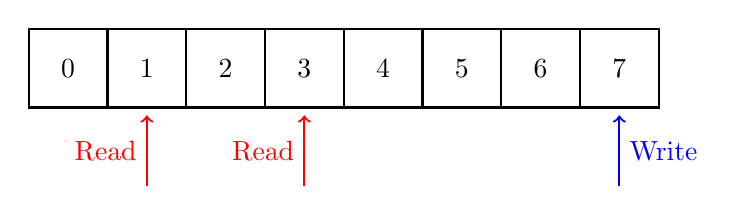
\begin{tikzpicture}
\foreach \i in {0,1,2,3,4,5,6,7} {
    \draw[thick] (\i,0) rectangle (\i+1,1); % Draw each spot in the queue
    \node at (\i+0.5, 0.5) {\i}; % Label each spot
}
\draw[thick, ->, red] (1.5, -1) -- (1.5, -0.1) node[midway, left] {Read};
\draw[thick, ->, red] (3.5, -1) -- (3.5, -0.1) node[midway, left] {Read}; % Added read pointer at position 3
\draw[thick, ->, blue] (7.5, -1) -- (7.5, -0.1) node[midway, right] {Write};
\end{tikzpicture}
\end{center}

\section{Design}

Some of the design limitation include:
\begin{itemize}
    \item A resource is exclusively updated by one owner, and read by one or more readers
    \item For shared resource that can be updated by multiple owners, the CPU
    can guarantee exclusive update from a single resource 
\end{itemize}

For the design:
\begin{itemize}
    \item SPMC is implemented as a circular queue with size of N
    \item The status of individual index is represented as a status array of size N
    \item The status of each index is either UNUSED, WRITTEN, or READING
    \item Each reader maintain its own read pointer
    \item A \textit{outstanding} counter is incremented by the writer when write is complete, 
    and decremented by the reader when it reserves a read
\end{itemize}

Whenever the write finishes a write, it increments \textit{outstanding} to
indicate some buffer is ready to read.\newline 

To read, a reader performs a two-step reservation: 
\begin{itemize}
    \item The reader decrements \textit{outstanding}. A successful decrement means
    the reader is \textit{guaranteed} a read index.
    \item After successful decrement of \textit{outstanding}, the reader walk
    its read pointer until it successfully reserve the next available index to
    read. This is done by attempting to CAS update an index from \textit{WRITTEN} to
    \textit{READING}. If the update fails, then the index was already reserved by another 
    reader.
\end{itemize}

There may be more than one approach in implementing SPMC, the above description
is what we will implement in this chapter.

\section{Spec}

The following is the core reader implementation:
\newline
\begin{pcal}
procedure reader() 
variable 
    i = self;
begin
r_chk_empty:        
    if outstanding # 0 then 
        outstanding := outstanding - 1; 
    else 
    r_early_ret:            
        return;
    end if;
r_try_lock:         
    if status[rptr[i]] = WRITTEN then 
        status[rptr[i]] := READING;
    else 
    r_retry:                
        rptr[i] := (rptr[i] + 1) % N;
            goto r_try_lock;
    end if;
r_data_chk:         
    assert buffer[rptr[i]] = rptr[i] + 1000;
r_read_buf:         
    buffer[rptr[i]] := 0;
r_unlock:           
    status[rptr[i]] := UNUSED;
r_done:             
    return;
end procedure; 
\end{pcal}
\begin{tlatex}
\@x{ {\p@procedure} reader {\p@lparen} {\p@rparen}}%
\@x{ {\p@variable}}%
\@x{\@s{16.4} i \.{=} self {\p@semicolon}}%
\@x{ {\p@begin}}%
\@x{ r\_chk\_empty\@s{.5}\textrm{:}\@s{3}}%
\@x{\@s{16.4} {\p@if} outstanding \.{\neq} 0 {\p@then}}%
\@x{\@s{20.5} outstanding \.{:=} outstanding \.{-} 1 {\p@semicolon}}%
\@x{\@s{16.4} {\p@else}}%
\@x{\@s{16.4} r\_early\_ret\@s{.5}\textrm{:}\@s{3}}%
\@x{\@s{32.8} {\p@return} {\p@semicolon}}%
\@x{\@s{16.4} {\p@end} {\p@if} {\p@semicolon}}%
\@x{ r\_try\_lock\@s{.5}\textrm{:}\@s{3}}%
\@x{\@s{16.4} {\p@if} status [ rptr [ i ] ] \.{=} WRITTEN {\p@then}}%
\@x{\@s{20.5} status [ rptr [ i ] ] \.{:=} READING {\p@semicolon}}%
\@x{\@s{16.4} {\p@else}}%
\@x{\@s{16.4} r\_retry\@s{.5}\textrm{:}\@s{3}}%
 \@x{\@s{32.8} rptr [ i ] \.{:=} ( rptr [ i ] \.{+} 1 ) \.{\%} N
 {\p@semicolon}}%
\@x{\@s{32.8} {\p@goto} r\_try\_lock {\p@semicolon}}%
\@x{\@s{16.4} {\p@end} {\p@if} {\p@semicolon}}%
\@x{ r\_data\_chk\@s{.5}\textrm{:}\@s{3}}%
 \@x{\@s{16.4} {\p@assert} buffer [ rptr [ i ] ] \.{=} rptr [ i ] \.{+} 1000
 {\p@semicolon}}%
\@x{ r\_read\_buf\@s{.5}\textrm{:}\@s{3}}%
\@x{\@s{16.4} buffer [ rptr [ i ] ] \.{:=} 0 {\p@semicolon}}%
\@x{ r\_unlock\@s{.5}\textrm{:}\@s{3}}%
\@x{\@s{16.4} status [ rptr [ i ] ] \.{:=} UNUSED {\p@semicolon}}%
\@x{ r\_done\@s{.5}\textrm{:}\@s{3}}%
\@x{\@s{16.4} {\p@return} {\p@semicolon}}%
\@x{ {\p@end} {\p@procedure} {\p@semicolon}}%
\end{tlatex}
\newline

The reader performs a non-zero check on outstanding. If the outstanding is zero,
the queue is empty, and the reader early returns.\\

If outstanding is K, then at most K readers can reserve an index to read. If system 
has M readers, then M-K readers will fail to reserve a read index. The readers now 
compete to reserve a read. More specifically: 
\begin{itemize}
    \item Reader loads outstanding, stores that onto local variable counter.
    \item Reader early returns if counter is zero 
    \item Reader attempts to update outstanding with CAS using counter and counter - 1.
    \item If CAS fails, go back to the top and retry.
\end{itemize}

If rv is non-success, another reader has \textit{won} the reservation. The
current reader can attempt to reserve again if \textit{outstanding} is
non-zero.\newline

If rv is a success, the reader is \textit{guaranteed} a read. However, readers
may still compete during index reservation. To reserve an index, a reader issues
CAS to update the index status from \textit{WRITTEN} to \textit{READING}. CAS
failure indicates another reader has already reserved this index. The reader
will bump the read pointer and try to reserve the next index.\\

Now let us take a look at the writer implementation:\\

\begin{pcal}
procedure writer() begin
w_chk_full:         
    if outstanding = N - 1 then 
    w_early_ret:            
        return; 
    end if;
w_chk_st:           
    if status[wptr] # UNUSED then 
    w_early_ret2:           
        return;
    end if;
w_write_buf:        
    buffer[wptr] := wptr + 1000;
w_mark_written:     
    status[wptr] := WRITTEN;
w_inc_wptr:         
    wptr := (wptr + 1) % N;
w_inc:              
    outstanding := outstanding + 1;
w_done:             
    return;
end procedure; 
\end{pcal}
\begin{tlatex}
\@x{ {\p@procedure} writer {\p@lparen} {\p@rparen} {\p@begin}}%
\@x{ w\_chk\_full\@s{.5}\textrm{:}\@s{3}}%
\@x{\@s{16.4} {\p@if} outstanding \.{=} N \.{-} 1 {\p@then}}%
\@x{\@s{16.4} w\_early\_ret\@s{.5}\textrm{:}\@s{3}}%
\@x{\@s{32.8} {\p@return} {\p@semicolon}}%
\@x{\@s{16.4} {\p@end} {\p@if} {\p@semicolon}}%
\@x{ w\_chk\_st\@s{.5}\textrm{:}\@s{3}}%
\@x{\@s{16.4} {\p@if} status [ wptr ] \.{\neq} UNUSED {\p@then}}%
\@x{\@s{16.4} w\_early\_ret2\@s{.5}\textrm{:}\@s{3}}%
\@x{\@s{32.8} {\p@return} {\p@semicolon}}%
\@x{\@s{16.4} {\p@end} {\p@if} {\p@semicolon}}%
\@x{ w\_write\_buf\@s{.5}\textrm{:}\@s{3}}%
\@x{\@s{16.4} buffer [ wptr ] \.{:=} wptr \.{+} 1000 {\p@semicolon}}%
\@x{ w\_mark\_written\@s{.5}\textrm{:}\@s{3}}%
\@x{\@s{16.4} status [ wptr ] \.{:=} WRITTEN {\p@semicolon}}%
\@x{ w\_inc\_wptr\@s{.5}\textrm{:}\@s{3}}%
\@x{\@s{16.4} wptr \.{:=} ( wptr \.{+} 1 ) \.{\%} N {\p@semicolon}}%
\@x{ w\_inc\@s{.5}\textrm{:}\@s{3}}%
\@x{\@s{16.4} outstanding \.{:=} outstanding \.{+} 1 {\p@semicolon}}%
\@x{ w\_done\@s{.5}\textrm{:}\@s{3}}%
\@x{\@s{16.4} {\p@return} {\p@semicolon}}%
\@x{ {\p@end} {\p@procedure} {\p@semicolon}}%
\end{tlatex}
\newline

The writer first checks outstanding, and early return if queue is full. After
fullness check, the writer then checks if the current index is UNUSED.  This is
to account for the edge case where a reader has performed the reservation first
step to decrement outstanding but haven't done the actual read. If both checks
pass, then writer now has an UNUSED index it can write to.\newline

The SPMC algorithm can be tricky to get right. There are many things to consider when 
designing a SPMC queue. Considerations include:
\begin{itemize}
    \item Readers can lapse each other
    \item Readers can lapse writer 
    \item One reader can starve other readers
    \item A slow reader can block the system
\end{itemize}

And under all circumstances, system \textit{correctness} must be maintained.

\section{Safety}

When a reader reserves an index to read, the reader must have exclusive access. 
This can be described as: For any pair of readers inside critical section, they
must operate on different indices:\newline

\begin{tla}
ExclusiveReservation == 
    \A x, y \in READERS: 
        (x /= y /\ pc[x] = "r_read_buf" /\ pc[y] = "r_read_buf") 
            => (rptr[x] # rptr[y])
\end{tla}
\begin{tlatex}
\@x{ ExclusiveReservation \.{\defeq}}%
\@x{\@s{16.4} \A\, x ,\, y \.{\in} READERS \.{:}}%
 \@x{\@s{16.4} ( x \.{\neq} y \.{\land} pc [ x ] \.{=}\@w{r\_read\_buf}
 \.{\land} pc [ y ] \.{=}\@w{r\_read\_buf} )}%
\@x{\@s{20.5} \.{\implies} ( rptr [ x ] \.{\neq} rptr [ y ] )}%
\end{tlatex}
\newline

Similarly, for any reader and writer inside critical section, they musut operate
on different indices as well:\newline
\begin{tla}
ExclusiveReadWrite == 
    \A x \in READERS: 
        (pc[x] = "r_read_buf" /\ pc[WRITER] = "w_write_buf") => (rptr[x] # wptr)
\end{tla}
\begin{tlatex}
\@x{ ExclusiveReadWrite \.{\defeq}}%
\@x{\@s{16.4} \A\, x \.{\in} READERS \.{:}}%
 \@x{\@s{20.5} ( pc [ x ] \.{=}\@w{r\_read\_buf} \.{\land} pc [ WRITER ]
 \.{=}\@w{w\_write\_buf} ) \.{\implies} ( rptr [ x ] \.{\neq} wptr )}%
\end{tlatex}

\section{Liveness}

All indices must be used as the system runs. The following verifies all unused
indices are eventually used, and all used indicies are eventually unused:
\newline
\begin{tla}
Liveness ==
    /\ \A k \in 0..N-1:
        buffer[k] = 0 ~> buffer[k] # 0
    /\ \A k \in 0..N-1:
        buffer[k] # 0 ~> buffer[k] = 0
\end{tla}
\begin{tlatex}
\@x{ Liveness \.{\defeq}}%
\@x{\@s{16.4} \.{\land} \A\, k \.{\in} 0 \.{\dotdot} N \.{-} 1 \.{:}}%
\@x{\@s{20.5} buffer [ k ] \.{=} 0 \.{\leadsto} buffer [ k ] \.{\neq} 0}%
\@x{\@s{16.4} \.{\land} \A\, k \.{\in} 0 \.{\dotdot} N \.{-} 1 \.{:}}%
\@x{\@s{20.5} buffer [ k ] \.{\neq} 0 \.{\leadsto} buffer [ k ] \.{=} 0}%
\end{tlatex}
\newline

The following describes a more subtle scenario. We need to ensure the system
remains functional even if readers complete out-of-order. The following describe
such scenario, where two non-contiguous indicies have been reserved for reading.
In this case we expect the indicies to eventually be re-used. This means the
system remains functional after such scenario.\newline

\begin{tla}
Liveness2 == 
    \A k \in 0..N-3:
    /\ (status[k] = READING /\ status[k+1] = UNUSED /\ status[k+2] = READING)
        ~> (status[k] = WRITTEN)
    /\ (status[k] = READING /\ status[k+1] = UNUSED /\ status[k+2] = READING)
        ~> (status[k+2] = WRITTEN)
\end{tla}
\begin{tlatex}
\@x{ Liveness2 \.{\defeq}}%
\@x{\@s{16.4} \A\, k \.{\in} 0 \.{\dotdot} N \.{-} 3 \.{:}}%
 \@x{\@s{16.4} \.{\land} ( status [ k ] \.{=} READING \.{\land} status [ k
 \.{+} 1 ] \.{=} UNUSED \.{\land} status [ k \.{+} 2 ] \.{=} READING )}%
\@x{\@s{16.4} \.{\leadsto} ( status [ k ] \.{=} WRITTEN )}%
 \@x{\@s{16.4} \.{\land} ( status [ k ] \.{=} READING \.{\land} status [ k
 \.{+} 1 ] \.{=} UNUSED \.{\land} status [ k \.{+} 2 ] \.{=} READING )}%
\@x{\@s{16.4} \.{\leadsto} ( status [ k \.{+} 2 ] \.{=} WRITTEN )}%
\end{tlatex}

% \end{document}


\part{System Modeling}

Specifications described so far have been designed to with finite state space to
allow model checker to explore all states and prove correctness. In this
section, we will relax this and allow infinite state space.\\

This uses TLA+ as a \textit{prototyping} tool. By definition, the model checker
cannot verify infinite sate space. However, for all states it does explore, it
will verify safety properties and highlight all the violations. This enables
designer to quickly iterate on design to flesh out what may or may not work. Per
80/20 rule, the model checker will very quickly identify obvious violations in
the design.\\

Once settled on a design and model checker no longer reports violation in any 
practical amount of time, one can always reduce the specification into finite
space to exhaustively prove correctness. 

% \begin{document}

\usetikzlibrary{arrows.meta} % For double arrows

\chapter{KV Store with Cache}

LRU cache, or least-re cently-used cache, is a finite-sized cache that evicts 
the least-recently-used entry when full. Modern CPU architecture supports
multi-layer cache. Caches closer to the CPU are faster, but also smaller. Cache is 
designed to take advantage of temporal locality, where recently accessed data isgenerally likely to be re-accessed in near future.\\

Caches are also applied more broadly: CDNs (content delivery
networks) are a group of geographically distributed servers close to
users in different parts of the world. Redis is a high-performance in-memory
key-value store, effectively a cache layer without underlying storage. The list of
examples goes on and on.

\section{Design}

In this chapter, we will describe a simple key-value store with a fixed-sized 
write-back LRU cache. The size of the key-value store is assumed unbounded. LRUcache acts as a fast access buffer until it's full. When it's full, the
least-recently-used entry key-value pair is evicted into the main memory.\\

Similar to a system with a cache, a key may exist in both the cache and memory
with different values. The key-value pair in the cache is assumed up-to-date,
while the key-value pair in memory may be stale. When the key-value pair is
evicted from the cache, the key in memory is synchronized by write-back from
the cache.\\

We will implement three specifications in this chapter: LRU cache, KV store, and
Test, with one building on another. The KV store is implemented using the LRU
cache, and Test verifies the KV stores.

\section{LRU Cache}

LRU cache can be implemented using three data structures: 
\begin{itemize}
    \item Linked list to track key access recency 
    \item Lookup table to track key and recency list iterator 
    \item Lookup table to track the key-value pair
\end{itemize}

Recency list is a doubly-linked list where the most recently accessed item is at
the tail. On read or write of an existing key, the key/iterator lookup table is
used to identify the key to update. The identified key is then moved to the tail
of the recency list to indicate recent access. Finally, the key-value table is
updated if needed. When inserting a new key-value pair, the head of the recency list
is evicted to make space, if required.\\

When specifying the LRU cache with TLA+, we can omit the key/iterator table to
simplify the specification. Recency list can be implemented as a \textit{tuple},
and a key-value table as a \textit{function}.\\

\subsection{Spec}

The following implements the LRU put function:\\

\begin{tla}
Put(k, v) == 
    IF k \in DOMAIN lru_kv THEN 
        \* replace
        /\ lru_recency' = Append(SelectSeq(lru_recency, LAMBDA x : x # k), k)
        /\ lru_kv' = [n \in DOMAIN lru_kv |-> IF n = k THEN v ELSE lru_kv[n]]
        /\ UNCHANGED lru_size
    ELSE 
        IF Len(lru_recency) # lru_size THEN 
            \* add 
            /\ lru_recency' = Append(lru_recency, k)
            /\ lru_kv' = [n \in DOMAIN lru_kv \cup {k} |-> n]
            /\ UNCHANGED lru_size
        ELSE 
            \* replace oldest 
            /\ lru_recency' = Append(SelectSeq(lru_recency,         
                                LAMBDA x : x # lru_recency[1]), k)
            /\ lru_kv' = [n \in (DOMAIN lru_kv \cup {k}) \ {lru_recency[1]} |-> 
                            IF n # k THEN lru_kv[n] ELSE v]
            /\ UNCHANGED lru_size
\end{tla}
\begin{tlatex}
\@x{ Put ( k ,\, v ) \.{\defeq}}%
\@x{ {\IF} k \.{\in} {\DOMAIN} lru\_kv \.{\THEN}}%
\@x{\@s{4.1}}%
\@y{%
  replace
}%
\@xx{}%
 \@x{\@s{4.1} \.{\land} lru\_recency \.{'} \.{=} Append ( SelectSeq (
 lru\_recency ,\, {\LAMBDA} x \.{:} x \.{\neq} k ) ,\, k )}%
 \@x{\@s{4.1} \.{\land} lru\_kv \.{'} \.{=} [ n \.{\in} {\DOMAIN} lru\_kv
 \.{\mapsto} {\IF} n \.{=} k \.{\THEN} v \.{\ELSE} lru\_kv [ n ] ]}%
\@x{\@s{4.1} \.{\land} {\UNCHANGED} lru\_size}%
\@x{ \.{\ELSE}}%
\@x{\@s{16.4} {\IF} Len ( lru\_recency ) \.{\neq} lru\_size \.{\THEN}}%
\@x{\@s{20.5}}%
\@y{%
  add 
}%
\@xx{}%
 \@x{\@s{20.5} \.{\land} lru\_recency \.{'} \.{=} Append ( lru\_recency ,\, k
 )}%
 \@x{\@s{20.5} \.{\land} lru\_kv \.{'} \.{=} [ n \.{\in} {\DOMAIN} lru\_kv
 \.{\cup} \{ k \} \.{\mapsto} n ]}%
\@x{\@s{20.5} \.{\land} {\UNCHANGED} lru\_size}%
\@x{\@s{16.4} \.{\ELSE}}%
\@x{\@s{32.8}}%
\@y{%
  replace oldest 
}%
\@xx{}%
 \@x{\@s{32.8} \.{\land} lru\_recency \.{'} \.{=} Append ( SelectSeq (
 lru\_recency ,\,}%
\@x{\@s{41.0} {\LAMBDA} x \.{:} x \.{\neq} lru\_recency [ 1 ] ) ,\, k )}%
 \@x{\@s{32.8} \.{\land} lru\_kv \.{'} \.{=} [ n \.{\in} ( {\DOMAIN} lru\_kv
 \.{\cup} \{ k \} ) \.{\,\backslash\,} \{ lru\_recency [ 1 ] \} \.{\mapsto}}%
\@x{\@s{32.8} {\IF} n \.{\neq} k \.{\THEN} lru\_kv [ n ] \.{\ELSE} v ]}%
\@x{\@s{32.8} \.{\land} {\UNCHANGED} lru\_size}%
\end{tlatex}
\\

When the implementation needs to extract a key and move it to the end, it uses
\textit{SelectSeq} to remove the targeted key and \textit{Append} to append the
key to the end. When updating \textit{lru\_kv}, the keyspace is expanded with
\textit{k}. In the case keyspace is full, then \textit{lru\_recency[1]} (least 
recent entry in LRU) is evicted.

\subsection{Safety}

For safety, we want to ensure values in \textit{lru\_recency} match with keys
in \textit{lru\_function}. Similarly, LRU size cannot exceed \textit{lru\_size}.\\

\begin{tla}
    Consistent ==
    /\ {lru_recency[k] : k \in DOMAIN lru_recency} = DOMAIN lru_kv
    /\ Cardinality(DOMAIN lru_kv) <= lru_size
\end{tla}
\begin{tlatex}
\@x{\@s{16.4} Consistent \.{\defeq}}%
 \@x{\@s{16.4} \.{\land} \{ lru\_recency [ k ] \.{:} k \.{\in} {\DOMAIN}
 lru\_recency \} \.{=} {\DOMAIN} lru\_kv}%
\@x{\@s{16.4} \.{\land} Cardinality ( {\DOMAIN} lru\_kv ) \.{\leq} lru\_size}%
\end{tlatex}

\subsection{Liveness}

There isn't any notable converging property for the LRU cache. Omitted from this chapter. 

\section{KV Store}

The KV store itself is pretty straightforward in design, naively we need a single 
\textit{function} to implement a table that holds the key-value pairs. The slight complexity 
is integrating LRU into the KV store. This is described in the \textit{Update} function:

\begin{tla}
Update(k, v) == 
    IF LRU!Contains(k) THEN 
         /\ LRU!Put(k, v)
         /\ UNCHANGED kv
         /\ latency' = CACHED
    ELSE \* LRU does not contain k
        /\ IF LRU!IsFull THEN 
                LET 
                    pair == LRU!GetLeastRecent
                    key == CHOOSE only \in DOMAIN pair: TRUE
                    value == pair[key]
                IN 
                    \* Evicted from LRU and write to memory
                    /\ kv' = [x \in DOMAIN kv \cup {key} |-> 
                                IF x = key THEN value ELSE kv[x]]
            ELSE 
                UNCHANGED kv 
        /\ LRU!Put(k, v)
        /\ latency' = EVICT
\end{tla}
\begin{tlatex}
\@x{ Update ( k ,\, v ) \.{\defeq}}%
\@x{\@s{16.4} {\IF} LRU {\bang} Contains ( k ) \.{\THEN}}%
\@x{\@s{24.59} \.{\land} LRU {\bang} Put ( k ,\, v )}%
\@x{\@s{24.59} \.{\land} {\UNCHANGED} kv}%
\@x{\@s{24.59} \.{\land} latency \.{'} \.{=} CACHED}%
\@x{\@s{16.4} \.{\ELSE}}%
\@y{%
  LRU does not contain k
}%
\@xx{}%
\@x{\@s{32.8} \.{\land} {\IF} LRU {\bang} IsFull \.{\THEN}}%
\@x{\@s{41.0} \.{\LET}}%
\@x{\@s{57.4} pair \.{\defeq} LRU {\bang} GetLeastRecent}%
 \@x{\@s{57.4} key \.{\defeq} {\CHOOSE} only \.{\in} {\DOMAIN} pair \.{:}
 {\TRUE}}%
\@x{\@s{57.4} value \.{\defeq} pair [ key ]}%
\@x{\@s{41.0} \.{\IN}}%
\@x{\@s{57.4}}%
\@y{%
  Evicted from LRU and write to memory
}%
\@xx{}%
 \@x{\@s{57.4} \.{\land} kv \.{'} \.{=} [ x \.{\in} {\DOMAIN} kv \.{\cup} \{
 key \} \.{\mapsto}}%
\@x{\@s{57.4} {\IF} x \.{=} key \.{\THEN} value \.{\ELSE} kv [ x ] ]}%
\@x{\@s{36.89} \.{\ELSE}}%
\@x{\@s{53.29} {\UNCHANGED} kv}%
\@x{\@s{32.8} \.{\land} LRU {\bang} Put ( k ,\, v )}%
\@x{\@s{32.8} \.{\land} latency \.{'} \.{=} EVICT}%
\end{tlatex}
\\

If the LRU contains the key (full or not), we simply update the LRU. The LRU will
update its internal recency list. If LRU doesn't contain the key, we have two
possible scenarios. If the LRU is not full, we can simply insert it into the LRU.
If the LRU is full, we need to evict the least recently used key-value pair 
write back to KV store, and insert the new key-value pair into the LRU.
\subsection{Safety}

Omitted.

\subsection{Liveness}

Omitted.

\section{Test}

Putting everything together, we want to characterize the design and
confirm wget get the expected latency improvement. 

\subsection{Spec}

The core of the test is pretty straightforward, we assume the usual 80/20 rule
where 80\% of the traffic are cache hits and 20\% are cache misses. This can be
simulated using the existential qualifier:\\

\begin{tla}
Next ==
    \/ \E p \in 1..10:
        /\  IF p > 2 THEN
                \* cached
                /\ \E k \in DOMAIN lru_kv:
                    /\ KV!Update(k, lru_kv[k])
                    /\ written' = [x \in DOMAIN written \ {k} |-> 
                                    IF x = k THEN k ELSE written[x]]
            ELSE 
                \* cache miss
                \* /\ PrintT(p)
                /\ \E k \in DataSet \ DOMAIN lru_kv:
                    /\ KV!Update(k, k)
                    /\ written' = [x \in DOMAIN written \ {k} |-> 
                                    IF x = k THEN k ELSE written[x]]
\end{tla}
\begin{tlatex}
\@x{ Next \.{\defeq}}%
\@x{\@s{16.4} \.{\lor} \E\, p \.{\in} 1 \.{\dotdot} 10 \.{:}}%
\@x{\@s{20.5} \.{\land}\@s{4.1} {\IF} p \.{>} 2 \.{\THEN}}%
\@x{\@s{28.7}}%
\@y{%
  cached
}%
\@xx{}%
\@x{\@s{28.7} \.{\land} \E\, k \.{\in} {\DOMAIN} lru\_kv \.{:}}%
\@x{\@s{32.8} \.{\land} KV {\bang} Update ( k ,\, lru\_kv [ k ] )}%
 \@x{\@s{32.8} \.{\land} written \.{'} \.{=} [ x \.{\in} {\DOMAIN} written
 \.{\,\backslash\,} \{ k \} \.{\mapsto}}%
\@x{\@s{36.89} {\IF} x \.{=} k \.{\THEN} k \.{\ELSE} written [ x ] ]}%
\@x{\@s{24.6} \.{\ELSE}}%
\@x{\@s{41.0}}%
\@y{%
  cache miss
}%
\@xx{}%
\@x{\@s{41.0}}%
\@y{%
  /\ PrintT(p)
}%
\@xx{}%
 \@x{\@s{41.0} \.{\land} \E\, k \.{\in} DataSet \.{\,\backslash\,} {\DOMAIN}
 lru\_kv \.{:}}%
\@x{\@s{45.1} \.{\land} KV {\bang} Update ( k ,\, k )}%
 \@x{\@s{45.1} \.{\land} written \.{'} \.{=} [ x \.{\in} {\DOMAIN} written
 \.{\,\backslash\,} \{ k \} \.{\mapsto}}%
\@x{\@s{49.19} {\IF} x \.{=} k \.{\THEN} k \.{\ELSE} written [ x ] ]}%
\end{tlatex}
\\

\subsection{Safety}

We want to verify the KV store with cache returns the correct value for 
all the key-value pairs written:\\

\begin{tla}
Consistent == 
    \A k \in DOMAIN written: 
        KV!Read(k) = written[k]
\end{tla}
\begin{tlatex}
\@x{ Consistent \.{\defeq}}%
\@x{\@s{16.4} \A\, k \.{\in} {\DOMAIN} written \.{:}}%
\@x{\@s{20.5} KV {\bang} Read ( k ) \.{=} written [ k ]}%
\end{tlatex}

\subsection{Liveness}

Omitted.

\section{Statistical Sampling}

To collect statistical latency numbers for the design, include the Community
Module CSV and define Safety property:\\

\begin{tla}
CSVFile ==
    "stat.csv"

Stats ==
    /\ CSVWrite("%1$s", <<latency>>, CSVFile)
\end{tla}
\begin{tlatex}
\@x{ CSVFile \.{\defeq}}%
\@x{\@s{16.4}\@w{stat.csv}}%
\@pvspace{8.0pt}%
\@x{ Stats \.{\defeq}}%
 \@x{\@s{16.4} \.{\land} CSVWrite (\@w{\%1\$s} ,\, {\langle} latency {\rangle}
 ,\, CSVFile )}%
\end{tlatex}
\\

The Safety property \textit{Stats} will be triggered in every state, collecting
the latency number in a .csv. To generate the .csv: 

\begin{verbatim}
rm -rf *.csv 
    && java -cp tla2tools.jar tlc2.TLC \
        -generate -note ~/dev/tla/tla/test_kv
\end{verbatim}

The latency numbers have now been collected into stat.csv. Now let us count the
latency numbers:

\begin{verbatim}
cat stat.csv  | grep 10 -ws | wc 
    && cat stat.csv  | grep 100 -ws | wc

  34674   34674  104022
   9239    9239   36956
\end{verbatim}

With a total of 43913 samples, cache hit happens about 78.9\% of the time. This 
closely matches the desired 80\% cache hit defined in the test.

% \end{document}




SPECIFICATION
    Spec

INVARIANTS 
    \* Consistent
    Consistent2
    \* Type_OK

PROPERTIES 
    \* AlwaysEventually
    \* EventuallyAlways
    \* LeadsTo


% \begin{document}

\usetikzlibrary{arrows.meta} % For double arrows

\chapter{Decentralized Database}

In the era of big-data today, localized instance of relational database is no
longer enough to hold the volume of data for toady's requirement. Distributed
key-value store has been of a key area of interest in the past few decades. 
Offering such as DynamoDB, Cassandra, Azure Cloud are a few examples of what
industry leaders are offering to address the data problem.\\

Service provided by a distributed key-value store is collectively offered by a
cluster of nodes. The nodes independently restart, update, crash, join or leave 
the cluster, while the service remains uninterrupted (though with possibly
reduced service). As the user base scales, the service must scale accordingly.\\

Two of the key design principles in a distributed data are partition and
replication.\\

A replica group (RG) is a group of nodes that maintain the same set of data.
Nodes in a RG often spans multiple availability zone (AZ) to maximize uptime.
In case of a regional value that wipes out an entire AZ, the other nodes in the
RG can still maintain the service albeit at reduced QoS. The nodes in the RG are
kept in sync using consensus protocol such as Raft. Typically, a write is only
considered complete and ack'd to client once it has been recorded by the
majority of nodes in the RG.

Partition is a way to split the keyspace into slices. When the keyspace is
partitioned, a RG is only responsible for a slice of the keyspace. Bandwidth
demand is also amortized across all RGs. Partition is typically done using 
consistent hashing. Different from traditional hashing, consistent hashing
minimizes data movement when nodes join and leave the clusters. Consistent
hashing will be covered in detail in a later part of the chapter.\\

Some of the early distributed database design requires a centralized server for
meta management (eg. ZooKeeper). In this chapter, we will specify a fully
decentralized key-value store. To simplify the specification, we will assume 
each node itself is a functioning RG with associated reliability property (this
is considered a solved problem with Raft).This chapter will focus on system
behavior correctness as RGs join or leave the cluster and associated data
migration.

\section{Consistent Hashing}

Before we dive into design detail, we must first describe consistent hashing.
With a traditional hashing algorithm, changing the size of the hash space
requires data movement of the entire cluster. This is very undesirable.
Consistent hashing was introduced to minimize data movement, where movement is
only required when adding or removing nodes in the affected range. 

In consistent hashing, the hash space is assumed to be a ring, where the largest
hash value plus one wraps around to the hash of 0. Servers in a consistent
hashing cluster take up different ranges in the ring. For a given request, the
client where the request lands by hashing the request first, then walks the ring
clockwise until it finds a server. \\ 

Assume the following example:

\begin{center}
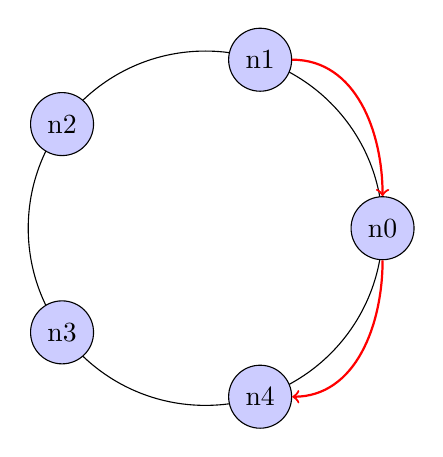
\begin{tikzpicture}[scale=1.5]

    \draw (0,0) circle (1.5cm);

    Draw the nodes on the circle with updated labels
    \foreach \angle/\label in {0/n0, 72/n1, 144/n2, 216/n3, 288/n4} {
        \node[draw, circle, fill=blue!20, minimum size=8mm] at (\angle:1.5cm) (\label) {\label};
    }

    \draw[->, thick, red] (n1) to[out=0, in=90] (n0); % 2 -> 1
    \draw[->, thick, red] (n0) to[out=270, in=0] (n4); % 1 -> 5

\end{tikzpicture}
\end{center}

If the request lands between n1 (exclusive) and n0 (inclusive), the request will
be processed by n0. Similarly, if the request lands between n0 (exclusive) and
n4 (inclusive), the request is to be processed by n4.\\

Assume a case where n4 goes offline: 

\begin{center}
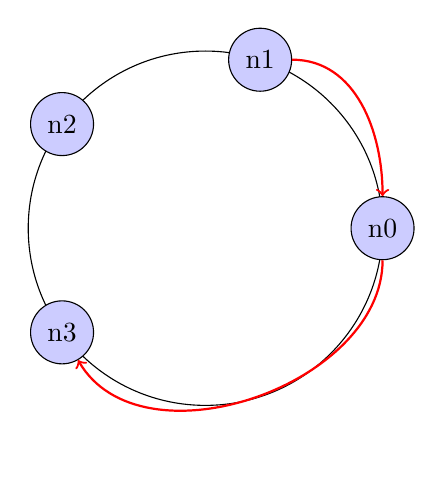
\begin{tikzpicture}[scale=1.5]

    \draw (0,0) circle (1.5cm);

    % Draw the nodes on the circle with updated labels
    \foreach \angle/\label in {0/n0, 72/n1, 144/n2, 216/n3} {
        \node[draw, circle, fill=blue!20, minimum size=8mm] at (\angle:1.5cm) (\label) {\label};
    }

    \draw[->, thick, red] (n1) to[out=0, in=90] (n0); % 2 -> 1
    \draw[->, thick, red] (n0) to[out=270, in=300] (n3); % 1 -> 5

\end{tikzpicture}
\end{center}

In such a case, requests previously processed by n4 will land on n3 instead.
Similarly, if a new node n5 is added:

\begin{center}
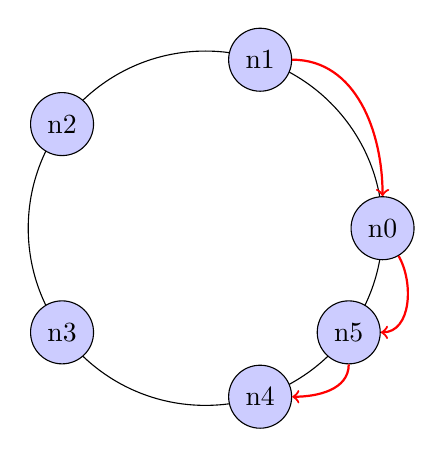
\begin{tikzpicture}[scale=1.5]

    % Draw the circle
    \draw (0,0) circle (1.5cm);

    % Draw the nodes on the circle with updated labels
    \foreach \angle/\label in {0/n0, 72/n1, 144/n2, 216/n3, 288/n4, 324/n5} {
        \node[draw, circle, fill=blue!20, minimum size=8mm] at (\angle:1.5cm) (\label) {\label};
    }

    % Draw arrows
    \draw[->, thick, red] (n1) to[out=0, in=90] (n0); % n1 -> n0
    \draw[->, thick, red] (n0) to[out=300, in=0] (n5); % n0 -> n4
    \draw[->, thick, red] (n5) to[out=270, in=0] (n4); % n0 -> n4

\end{tikzpicture}
\end{center}

Part of what n4 used to service will now be serviced by n5.

\section{Gossip Protocol}

Without a centralized metadata controller, the nodes learn about the peers using
gossip protocol. As a new RG enters the cluster, the design relies on gossip
protocol to spread the information. This is a critical part of the design as
will be described later.

\section{Design}

In our design, a RG can be in one of the following states: Offline, Joining,
Online, Leaving. The service starts with a single RG responsible for the entire
hash space. Since this is the epoch RG, it directly transitions into Online
state and can claim any token on the ring. For simplicity, epoch RG always claim
token 0.\\

The design assumes node failure handling are handled within the RG, the
specification will not model RG crash or restart. 

\subsection{Offline}

RG is offline, no impact to cluster.

\subsection{Joining}

By definition, the goal of adding a RG U into the cluster is to reduce the load
on another RG V. Since RG U is a new member of the cluster, it may not have the
latest cluster topology. Once RG U announces its presence via gossip protocol,
it waits for RG V to reach out.\\

When RG V realizes a new RG can share its burden, RG V will coordinate with RG U
to migrate a subset of its data to RG U (the subset RG U will be responsible
for). Once data migration completes: RG U transitions to Online state and start
servicing request in its range, while RG V rejects request to the range RG U has
taken over. This range update is also reflected in both RG U and V's local ring
cache, and communicated during next round of gossip protocol.

\subsection{Online}

RG is \textit{Online} and responds and records requests in its hash range. 

\subsection{Leaving}

Symmetrically, when a RG U is leaving the cluster, a RG V needs to take over the
range and data RG U is currently responsible for. Similarly to join, RG U 
announce its intent to leave, and wait for RG V to reach out and coordinate the
hand off.\\

Note when RG U is still waiting or in the middle of hand-off, it is still
\textit{Online} and must respond to request, until RV V fully takes over.

% Note this is a \textit{graceful} hand-off. The design assumes any failure
% mitigation is implemented within the RG. 


% Since the entire hash space is always covered by the cluster, a RG U joining 
% the cluster needs to coordinate with another RG V to take over part of RG V's 
% hash space. 
% take over a certain hash range needs to coordinate with RG V which is currently 
% responsible for that 
% cluster needs to coordinate with RG V that is currently responsible for the
% range. When RG U joins the cluster, it will announce its presence via gossip
% protocol. Eventually RG V will realize it can volunteer a part of its range to
% RG U, and 


% In this chapter, we will implement a simple distributed key-value store that
% supports horizontal scale-out. The service provider can add servers into the
% cluster dynamically to reduce the load on individual servers. Similarly, the
% service provider can also remove servers dynamically during off hours to
% minimize server costs.\\

% A new server \textit{K} joining the cluster claims a token \textit{T} on the
% ring. Starting from \textit{T}, walk the ring counter-clockwise to find the
% first neighboring token \textit{P}, \textit{K} owns the range of keys from
% \textit{P} (exclusive) to \textit{T} (inclusive).\\

% The design does not include replication or fault recovery to limit the scope.

\section{Specification}

\textit{Init} is defined below:\\

\begin{tla}
offline == [k \in RGState |-> 
            IF k = "version" THEN 0 
            ELSE IF k = "token" THEN -1
            ELSE IF k = "state" THEN "offline"
            ELSE "unused"]
seed == [k \in RGState |-> 
            IF k = "version" THEN 1 
            ELSE IF k = "token" THEN 0
            ELSE IF k = "state" THEN "online"
            ELSE "unused"]
Init ==
    /\ local_ring = [i \in RGs |-> 
                        [j \in RGs |-> 
                            IF i = SeedRG /\ j = SeedRG
                            THEN seed
                            ELSE offline ]] 
    /\ local_kv = [i \in RGs |-> {}]
    /\ debug_kv = {}
    /\ debug = {}
\end{tla}
\begin{tlatex}
\@x{ offline \.{\defeq} [ k \.{\in} RGState \.{\mapsto}}%
\@x{ {\IF} k \.{=}\@w{version} \.{\THEN} 0}%
\@x{ \.{\ELSE} {\IF} k \.{=}\@w{token} \.{\THEN} \.{-} 1}%
\@x{ \.{\ELSE} {\IF} k \.{=}\@w{state} \.{\THEN}\@w{offline}}%
\@x{ \.{\ELSE}\@w{unused} ]}%
\@x{ seed \.{\defeq} [ k \.{\in} RGState \.{\mapsto}}%
\@x{\@s{4.1} {\IF} k \.{=}\@w{version} \.{\THEN} 1}%
\@x{\@s{4.1} \.{\ELSE} {\IF} k \.{=}\@w{token} \.{\THEN} 0}%
\@x{\@s{4.1} \.{\ELSE} {\IF} k \.{=}\@w{state} \.{\THEN}\@w{online}}%
\@x{\@s{4.1} \.{\ELSE}\@w{unused} ]}%
\@x{ Init \.{\defeq}}%
\@x{\@s{16.4} \.{\land} local\_ring \.{=} [ i \.{\in} RGs \.{\mapsto}}%
\@x{\@s{20.5} [ j \.{\in} RGs \.{\mapsto}}%
\@x{\@s{24.6} {\IF} i \.{=} SeedRG \.{\land} j \.{=} SeedRG}%
\@x{\@s{24.6} \.{\THEN} seed}%
\@x{\@s{24.6} \.{\ELSE} offline ] ]}%
\@x{\@s{16.4} \.{\land} local\_kv \.{=} [ i \.{\in} RGs \.{\mapsto} \{ \} ]}%
\@x{\@s{16.4} \.{\land} debug\_kv \.{=} \{ \}}%
\@x{\@s{16.4} \.{\land} debug \.{=} \{ \}}%
\end{tlatex}
\\

Since RGs operate independently, each RG maintain its view of the ring. This is
tracked by \textit{local\_ring}. The cluster is initialized with a single RG
\textit{SeedRG} with \textit{version} set to 1, \textit{state} set to online and
claims \textit{token} 0 on the ring.\\

\textit{local\_kv} represents the per RG KV store. \textit{debug\_kv} records
what the client has written, this is used to verify consistency of the
distributed database. Finally, a \textit{debug} variable is used to hold a token
in a failure trace.\\

The core set of actions permitted by \textit{Spec} is defined below:\\
\begin{tla}
Next ==
    \/ \E u, v \in RGs:
        /\ Gossip(u, v)
    \/ \E u \in RGs:
        \/ Join(u) 
        \/ JoinMigrate(u)
        \/ Leave(u)
        \/ LeaveMigrate(u)
    \/ \E u \in RGs:
        /\ \E k \in KeySpace:
            /\ k \notin debug_kv
            /\ Write(u, k)
\end{tla}
\begin{tlatex}
\@x{ Next \.{\defeq}}%
\@x{\@s{16.4} \.{\lor} \E\, u ,\, v \.{\in} RGs \.{:}}%
\@x{\@s{20.5} \.{\land} Gossip ( u ,\, v )}%
\@x{\@s{16.4} \.{\lor} \E\, u \.{\in} RGs \.{:}}%
\@x{\@s{20.5} \.{\lor} Join ( u )}%
\@x{\@s{20.5} \.{\lor} JoinMigrate ( u )}%
\@x{\@s{20.5} \.{\lor} Leave ( u )}%
\@x{\@s{20.5} \.{\lor} LeaveMigrate ( u )}%
\@x{\@s{16.4} \.{\lor} \E\, u \.{\in} RGs \.{:}}%
\@x{\@s{20.5} \.{\land} \E\, k \.{\in} KeySpace \.{:}}%
\@x{\@s{24.6} \.{\land} k \.{\notin} debug\_kv}%
\@x{\@s{24.6} \.{\land} Write ( u ,\, k )}%
\end{tlatex}
\\

A RG can \textit{Join} or \textit{Leave} the cluster. However, both are graceful
operations requiring coordination of other nodes from the cluster. To complete
join or leave, another RG has to either offload of take over the range of the
joining or leaving RG.  This is described by \textit{JoinMigrate} and
\textit{LeaveMigrate}. Any pair of nodes can \textit{Gossip} to share their
understanding of the current cluster state. Finally, a client can \textit{Write}
to the database by sending request to a RG.\\

Let us take a look at definition for \textit{Join}:\\
\begin{tla}
ClaimedToken == 
    LET 
        not_offline == {v \in RGs: local_ring[v][v]["state"] # StateOffline}
    IN 
        {local_ring[k][k]["token"]: k \in not_offline}

Join(u) == 
    LET 
        key == CHOOSE any \in KeySpace \ ClaimedToken: TRUE
    IN 
        \* Only ever one node joining at a time
        /\ local_ring[u][u]["state"] = StateOffline
        /\ local_ring' = [local_ring EXCEPT ![u] 
                            = [local_ring[u] EXCEPT ![u]
                                = [k \in RGState |-> 
                                    IF k = "version" THEN local_ring[u][u][k] + 1
                                    ELSE IF k = "token" THEN key
                                    ELSE IF k = "state" THEN StatePrepare
                                    ELSE "unused"]]]
        /\ UNCHANGED <<local_kv, debug_kv, debug>>
\end{tla}
\begin{tlatex}
\@x{ ClaimedToken \.{\defeq}}%
\@x{\@s{16.4} \.{\LET}}%
 \@x{\@s{32.8} not\_offline \.{\defeq} \{ v \.{\in} RGs \.{:} local\_ring [ v
 ] [ v ] [\@w{state} ] \.{\neq} StateOffline \}}%
\@x{\@s{16.4} \.{\IN}}%
 \@x{\@s{32.8} \{ local\_ring [ k ] [ k ] [\@w{token} ] \.{:} k \.{\in}
 not\_offline \}}%
\@pvspace{8.0pt}%
\@x{ Join ( u ) \.{\defeq}}%
\@x{ \.{\LET}}%
 \@x{\@s{16.4} key \.{\defeq} {\CHOOSE} any \.{\in} KeySpace
 \.{\,\backslash\,} ClaimedToken \.{:} {\TRUE}}%
\@x{ \.{\IN}}%
\@x{\@s{16.4}}%
\@y{%
  Only ever one node joining at a time
}%
\@xx{}%
 \@x{\@s{16.4} \.{\land} local\_ring [ u ] [ u ] [\@w{state} ] \.{=}
 StateOffline}%
 \@x{\@s{16.4} \.{\land} local\_ring \.{'} \.{=} [ local\_ring {\EXCEPT}
 {\bang} [ u ]}%
\@x{\@s{24.59} \.{=} [ local\_ring [ u ] {\EXCEPT} {\bang} [ u ]}%
\@x{\@s{28.69} \.{=} [ k \.{\in} RGState \.{\mapsto}}%
 \@x{\@s{32.8} {\IF} k \.{=}\@w{version} \.{\THEN} local\_ring [ u ] [ u ] [ k
 ] \.{+} 1}%
\@x{\@s{32.8} \.{\ELSE} {\IF} k \.{=}\@w{token} \.{\THEN} key}%
\@x{\@s{32.8} \.{\ELSE} {\IF} k \.{=}\@w{state} \.{\THEN} StatePrepare}%
\@x{\@s{32.8} \.{\ELSE}\@w{unused} ] ] ]}%
 \@x{\@s{16.4} \.{\land} {\UNCHANGED} {\langle} local\_kv ,\, debug\_kv ,\,
 debug {\rangle}}%
\end{tlatex}
\\

A RG can only join the cluster if it is currently \textit{Offline}. To join the
cluster, the RG must claim an unclaimed token, enter \textit{Joining} state, and
announces its intent via \textit{Gossip}.\\

The design has taken a shortcut to claim an unclaimed token. In a production
implementation, a newly joined RG will not know which token is unclaimed. Since
the design relies on another RG to \textit{admit} the new RG into the cluster,
in the case of a collision the admitting RG can simply ask the RG that wishes to
join to pick a different token and restart the process. Practically, the hash
space is large enough that collision is unlikely.\\


The following describes \textit{JoinMigrate}:\\
\begin{tla}
RECURSIVE FindPrevToken(_, _)
FindPrevToken(key, ring) ==
    LET 
        condition(v) == ring[v]["state"] # StateOffline 
                    /\ ring[v]["token"] = key
        exists == \E v \in DOMAIN ring: condition(v)
        owner == CHOOSE only \in DOMAIN ring: condition(only)
    IN 
        IF exists THEN
            owner
        ELSE 
            FindPrevToken((key + N - 1) \% N, ring)

JoinMigrate(u) == 
    LET 
        \* previous token
        v == FindPrevToken((local_ring[u][u]["token"] + N - 1) % N, 
                            local_ring[u])
        all_keys == local_kv[u]
        all_online_tokens == AllOnlineTokens(u)
        v_token == local_ring[u][v]["token"]
        v_data == DataSet(v_token, all_online_tokens, all_keys)
        updated == [k \in RGState |-> 
                            IF k = "version" THEN local_ring[u][v]["version"] + 1
                            ELSE IF k = "token" THEN local_ring[u][v]["token"]
                            ELSE IF k = "state" THEN StateOnline
                            ELSE "unused"]
        merged == Merge(u, v)
        local_ring_u == [merged EXCEPT ![u] 
                            = [merged[u] EXCEPT ![v] = updated]]
        local_ring_uv == [local_ring_u EXCEPT ![v] 
                            = [local_ring_u[v] EXCEPT ![v] = updated]]
    IN 
        /\ Cardinality(AllTokens(u)) >= 2
        /\ local_ring[u][u]["state"] = StateOnline
        /\ local_ring[u][v]["state"] = StatePrepare
        /\ Cardinality(all_keys) # 0
        /\ IF v_data # {} THEN 
                /\ local_ring' = local_ring_uv
                /\ local_kv' = [k \in RGs |-> 
                                IF k = u THEN local_kv[k] \ v_data
                                ELSE IF k = v THEN local_kv[k] \cup v_data
                                ELSE local_kv[k]]
            ELSE 
                UNCHANGED <<local_ring, local_kv>>
        /\ UNCHANGED <<debug_kv, debug>>
\end{tla}
\begin{tlatex}
\@x{ {\RECURSIVE} FindPrevToken ( \_ ,\, \_ )}%
\@x{ FindPrevToken ( key ,\, ring ) \.{\defeq}}%
\@x{\@s{16.4} \.{\LET}}%
 \@x{\@s{32.8} condition ( v ) \.{\defeq} ring [ v ] [\@w{state} ] \.{\neq}
 StateOffline}%
\@x{\@s{36.89} \.{\land} ring [ v ] [\@w{token} ] \.{=} key}%
 \@x{\@s{32.8} exists \.{\defeq} \E\, v \.{\in} {\DOMAIN} ring \.{:} condition
 ( v )}%
 \@x{\@s{32.8} owner \.{\defeq} {\CHOOSE} only \.{\in} {\DOMAIN} ring \.{:}
 condition ( only )}%
\@x{\@s{16.4} \.{\IN}}%
\@x{\@s{32.8} {\IF} exists \.{\THEN}}%
\@x{\@s{36.89} owner}%
\@x{\@s{32.8} \.{\ELSE}}%
 \@x{\@s{49.19} FindPrevToken ( ( key \.{+} N \.{-} 1 ) \.{\,\backslash\,}
 \.{\%} N ,\, ring )}%
\@pvspace{8.0pt}%
\@x{ JoinMigrate ( u ) \.{\defeq}}%
\@x{\@s{16.4} \.{\LET}}%
\@x{\@s{32.8}}%
\@y{%
  previous token
}%
\@xx{}%
 \@x{\@s{32.8} v \.{\defeq} FindPrevToken ( ( local\_ring [ u ] [ u ]
 [\@w{token} ] \.{+} N \.{-} 1 ) \.{\%} N ,\,}%
\@x{\@s{32.8} local\_ring [ u ] )}%
\@x{\@s{32.8} all\_keys \.{\defeq} local\_kv [ u ]}%
\@x{\@s{32.8} all\_online\_tokens \.{\defeq} AllOnlineTokens ( u )}%
\@x{\@s{32.8} v\_token \.{\defeq} local\_ring [ u ] [ v ] [\@w{token} ]}%
 \@x{\@s{32.8} v\_data \.{\defeq} DataSet ( v\_token ,\, all\_online\_tokens
 ,\, all\_keys )}%
\@x{\@s{32.8} updated \.{\defeq} [ k \.{\in} RGState \.{\mapsto}}%
 \@x{\@s{41.0} {\IF} k \.{=}\@w{version} \.{\THEN} local\_ring [ u ] [ v ]
 [\@w{version} ] \.{+} 1}%
 \@x{\@s{41.0} \.{\ELSE} {\IF} k \.{=}\@w{token} \.{\THEN} local\_ring [ u ] [
 v ] [\@w{token} ]}%
\@x{\@s{41.0} \.{\ELSE} {\IF} k \.{=}\@w{state} \.{\THEN} StateOnline}%
\@x{\@s{41.0} \.{\ELSE}\@w{unused} ]}%
\@x{\@s{32.8} merged \.{\defeq} Merge ( u ,\, v )}%
\@x{\@s{32.8} local\_ring\_u \.{\defeq} [ merged {\EXCEPT} {\bang} [ u ]}%
\@x{\@s{45.1} \.{=} [ merged [ u ] {\EXCEPT} {\bang} [ v ] \.{=} updated ] ]}%
 \@x{\@s{32.8} local\_ring\_uv \.{\defeq} [ local\_ring\_u {\EXCEPT} {\bang} [
 v ]}%
 \@x{\@s{41.0} \.{=} [ local\_ring\_u [ v ] {\EXCEPT} {\bang} [ v ] \.{=}
 updated ] ]}%
\@x{\@s{16.4} \.{\IN}}%
\@x{\@s{32.8} \.{\land} Cardinality ( AllTokens ( u ) ) \.{\geq} 2}%
 \@x{\@s{32.8} \.{\land} local\_ring [ u ] [ u ] [\@w{state} ] \.{=}
 StateOnline}%
 \@x{\@s{32.8} \.{\land} local\_ring [ u ] [ v ] [\@w{state} ] \.{=}
 StatePrepare}%
\@x{\@s{32.8} \.{\land} Cardinality ( all\_keys ) \.{\neq} 0}%
\@x{\@s{32.8} \.{\land} {\IF} v\_data \.{\neq} \{ \} \.{\THEN}}%
\@x{\@s{41.0} \.{\land} local\_ring \.{'} \.{=} local\_ring\_uv}%
\@x{\@s{41.0} \.{\land} local\_kv \.{'} \.{=} [ k \.{\in} RGs \.{\mapsto}}%
 \@x{\@s{41.0} {\IF} k \.{=} u \.{\THEN} local\_kv [ k ] \.{\,\backslash\,}
 v\_data}%
 \@x{\@s{41.0} \.{\ELSE} {\IF} k \.{=} v \.{\THEN} local\_kv [ k ] \.{\cup}
 v\_data}%
\@x{\@s{41.0} \.{\ELSE} local\_kv [ k ] ]}%
\@x{\@s{36.89} \.{\ELSE}}%
\@x{\@s{53.29} {\UNCHANGED} {\langle} local\_ring ,\, local\_kv {\rangle}}%
\@x{\@s{32.8} \.{\land} {\UNCHANGED} {\langle} debug\_kv ,\, debug {\rangle}}%
\end{tlatex}

A RG U walks its local ring counter-clockwise to find the first neighboring RG
V. If RG V is in \textit{Joining} state, this allows RG U to offload part of
its range to RG V and admit RG V into the cluster. This coordination also
includes data migration, since some of the keys RG U have will be owned by RG V
as well. At the end of the process, both RG U and V update their local ring cache of
each others state, and propagate that in subsequent round of \textit{Gossip}.\\

In a practical implementation, the data migration process might take a while.
The RGs maintains merkle-trees for its data and uses that to determine
migration status. Once data migration completes, the range switch over is atomic. 
RG U stops servicing requests to the range RG V has taken over, and redirects 
the requests to RG V either explicitly or implicitly via gossip protocol.\\

The following defines \textit{Leave}:\\

\begin{tla}
Leave(u) == 
    LET 
        updated == [k \in RGState |-> 
                     IF k = "version" THEN local_ring[u][u][k] + 1
                     ELSE IF k = "token" THEN local_ring[u][u][k]
                     ELSE IF k = "state" THEN StateExit
                     ELSE "unused"]
    IN 
        \* can only leave if we are already online 
        /\ local_ring[u][u]["state"] = StateOnline
        \* can only leave if there's at least another server to migrate data to
        /\ Cardinality(AllOnlineTokens(u)) >= 2
        /\ local_ring' = [local_ring EXCEPT ![u] 
                            = [local_ring[u] EXCEPT ![u]
                                = updated]] 
        /\ UNCHANGED <<local_kv, debug_kv, debug>>
\end{tla}
\begin{tlatex}
\@x{ Leave ( u ) \.{\defeq}}%
\@x{\@s{16.4} \.{\LET}}%
\@x{\@s{32.8} updated \.{\defeq} [ k \.{\in} RGState \.{\mapsto}}%
 \@x{\@s{36.89} {\IF} k \.{=}\@w{version} \.{\THEN} local\_ring [ u ] [ u ] [
 k ] \.{+} 1}%
 \@x{\@s{36.89} \.{\ELSE} {\IF} k \.{=}\@w{token} \.{\THEN} local\_ring [ u ]
 [ u ] [ k ]}%
\@x{\@s{36.89} \.{\ELSE} {\IF} k \.{=}\@w{state} \.{\THEN} StateExit}%
\@x{\@s{36.89} \.{\ELSE}\@w{unused} ]}%
\@x{\@s{16.4} \.{\IN}}%
\@x{\@s{32.8}}%
\@y{%
  can only leave if we are already online 
}%
\@xx{}%
 \@x{\@s{32.8} \.{\land} local\_ring [ u ] [ u ] [\@w{state} ] \.{=}
 StateOnline}%
\@x{\@s{32.8}}%
\@y{%
  can only leave if there's at least another server to migrate data to
}%
\@xx{}%
\@x{\@s{32.8} \.{\land} Cardinality ( AllOnlineTokens ( u ) ) \.{\geq} 2}%
 \@x{\@s{32.8} \.{\land} local\_ring \.{'} \.{=} [ local\_ring {\EXCEPT}
 {\bang} [ u ]}%
\@x{\@s{41.0} \.{=} [ local\_ring [ u ] {\EXCEPT} {\bang} [ u ]}%
\@x{\@s{45.1} \.{=} updated ] ]}%
 \@x{\@s{32.8} \.{\land} {\UNCHANGED} {\langle} local\_kv ,\, debug\_kv ,\,
 debug {\rangle}}%
\end{tlatex}

Similar to \textit{Join}, a RG can leave if it is \textit{Online}, and not the
only RG in the cluster.


% \end{document}


\part{Reference}

\chapter{Fairness}
\label{chap:fairness}

For rigorous definition and proof, please refer to \cite{ss}. This chapter focus
on the application fairness by describing an elevator that eventually makes it to the 
top floor:\newline

\begin{center}
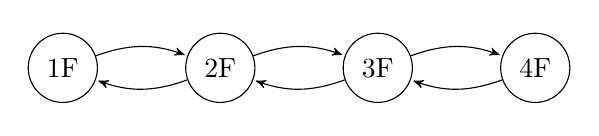
\begin{tikzpicture}[>=stealth',shorten >=1pt,auto,node distance=2cm]
  \node[state]  (q1)                {1F};
  \node[state]  (q2) [right of=q1]  {2F};
  \node[state]  (q3) [right of=q2]  {3F};
  \node[state]  (q4) [right of=q3]  {4F};

  \path[->]          (q1)  edge   [bend left=20]   node {} (q2);
  \path[->]          (q2)  edge   [bend left=20]   node {} (q1);

  \path[->]          (q2)  edge   [bend left=20]   node {} (q3);
  \path[->]          (q3)  edge   [bend left=20]   node {} (q2);

  \path[->]          (q3)  edge   [bend left=20]   node {} (q4);
  \path[->]          (q4)  edge   [bend left=20]   node {} (q3);

\end{tikzpicture}
\end{center}

\section{Liveness}

Consider the following elevator \textit{Spec}:
\begin{tla}
--------------------------- MODULE elevator ----------------------------
EXTENDS Integers
VARIABLES a
vars == <<a>>
TOP     == 4
BOTTOM  == 1
Init ==
    /\ a = BOTTOM
Up == 
    /\ a # TOP
    /\ a' = a + 1
Down == 
    /\ a # BOTTOM
    /\ a' = a - 1
Spec ==
  /\ Init
  /\ [][Up \/ Down]_a
=============================================================================
\end{tla}
\begin{tlatex}
\@x{}\moduleLeftDash\@xx{ {\MODULE} elevator}\moduleRightDash\@xx{}%
\@x{ {\EXTENDS} Integers}%
\@x{ {\VARIABLES} a}%
\@x{ vars \.{\defeq} {\langle} a {\rangle}}%
\@x{ TOP\@s{28.75} \.{\defeq} 4}%
\@x{ BOTTOM\@s{4.10} \.{\defeq} 1}%
\@x{ Init \.{\defeq}}%
\@x{\@s{16.4} \.{\land} a \.{=} BOTTOM}%
\@x{ Up \.{\defeq}}%
\@x{\@s{17.27} \.{\land} a \.{\neq} TOP}%
\@x{\@s{17.27} \.{\land} a \.{'} \.{=} a \.{+} 1}%
\@x{ Down \.{\defeq}}%
\@x{\@s{16.4} \.{\land} a \.{\neq} BOTTOM}%
\@x{\@s{16.4} \.{\land} a \.{'} \.{=} a \.{-} 1}%
\@x{ Spec \.{\defeq}}%
\@x{\@s{8.2} \.{\land}\@s{0.16} Init}%
\@x{\@s{8.2} \.{\land}\@s{0.16} {\Box} [ Up \.{\lor} Down ]_{ a}}%
\@x{}\bottombar\@xx{}%
\end{tlatex}

The building has a set of floors and the elevator can go either up or down. The
elevator keeps going up until it's the top floor, or keep going down until it's
the bottom floor. TLC will pass the spec as is.\newline

Let's introduce a liveness property. The elevator should always at least go 
to the second floor:\newline
\begin{tla}
Liveness == 
    /\ a = 1 ~> a = 2
\end{tla}
\begin{tlatex}
\@x{ Liveness \.{\defeq}}%
\@x{\@s{16.4} \.{\land} a \.{=} 1 \.{\leadsto} a \.{=} 2}%
\end{tlatex}
\newline

Model checker will report a violation on this property:

\begin{verbatim}
Error: Temporal properties were violated.
Error: The following behavior constitutes a counter-example:
State 1: <Initial predicate>
a = 1
State 2: Stuttering
\end{verbatim}

Since the \textit{Spec} permits \textit{suttering}, the state machine is allowed
to perpetually stay on 1F and \textit{never} go to 2F. This can be fixed by
introducing fairness description.

\section{Weak Fairness}

Weak fairness is defined as:\newline
\begin{equation} 
\Diamond\Box(ENABLED\langle A \rangle _v) \implies \Box\Diamond\langle A \rangle _v
\end{equation}
$ENABLED\langle A \rangle$ represents \textit{conditions required} for action A.
The above translates to: if conditions required for action A to occur is
\textit{eventually always} true, then action A will \textit{always eventually}
happen.\newline 

Without weak fairness defined, the elevator may \textit{stutter} at 1F and
never go to 2F. Weak fairness states that if the conditions of an action is
\textit{eventually always} true (ie. elevator decides to stay on 1F but 
\textit{can} go up), the elevator \textit{always eventually} go up.\newline

\begin{tla}
Spec ==
  /\ Init
  /\ [][Down \/ Up]_a
  /\ WF_a(Down)
  /\ WF_a(Up)
\end{tla}
\begin{tlatex}
\@x{ Spec \.{\defeq}}%
\@x{\@s{8.2} \.{\land}\@s{0.16} Init}%
\@x{\@s{8.2} \.{\land}\@s{0.16} {\Box} [ Down \.{\lor} Up ]_{ a}}%
\@x{\@s{8.2} \.{\land}\@s{0.16} {\WF}_{ a} ( Down )}%
\@x{\@s{8.2} \.{\land}\@s{0.16} {\WF}_{ a} ( Up )}%
\end{tlatex}
\newline

Running the spec against model checker passes again. What if we want to verify
the elevator eventually always goes to the top, not just to 2F? Let's modify the
Liveness property again:\newline
\begin{tla}
Liveness == 
    /\ a = BOTTOM ~> a = TOP
\end{tla}
\begin{tlatex}
\@x{ Liveness \.{\defeq}}%
\@x{\@s{16.4} \.{\land} a \.{=} BOTTOM \.{\leadsto} a \.{=} TOP}%
\end{tlatex}
\newline

Model checker now reports the following violation: 
\begin{verbatim}
Error: Temporal properties were violated.
Error: The following behavior constitutes a counter-example:
State 1: <Initial predicate>
a = 1
State 2: <Up line 10, col 5 to line 11, col 17 of module elevator>
a = 2
Back to state 1: <Down line 13, col 5 to line 14, col 17 of module elevator>
\end{verbatim}

Model checker identified a case where the elevator is perpetually stuck going
between 1F and 2F, but never go to 3F. Weak fairness is no longer enough,
because the the elevator is not stuck on 2F repeatedly, but stuck going
\textit{between} 1F and 2F. This is where we need strong fairness.

\section{Strong Fairness}

Strong fairness is defined as:\newline
\begin{equation} 
\Box\Diamond(ENABLED\langle A \rangle _v) \implies \Box\Diamond\langle A \rangle _v
\end{equation}
The difference between weak and strong fairness is the \textit{eventually
always} vs. \textit{always eventually}. \newline 

In weak fairness, once the state machine is stuck in a state forever, the state
machine always transition to a possible next state permitted by the
\textit{Spec} (eg. if the elevator is stuck on 1F but can go to 2F, it will).
With strong fairness, the elevator doesn't need to be stuck on 2F to go to 3F.
If the elevator \textit{always eventually} makes it to 2F, it \textit{always
eventually} go to 3F.\newline 

Intuitively we are tempted to enable strong fairness like so: \newline
\begin{tla}
Spec ==
  /\ Init
  /\ [][Up \/ Down]_a
  /\ WF_a(Down)
  /\ SF_a(UP)
\end{tla}
\begin{tlatex}
\@x{ Spec \.{\defeq}}%
\@x{\@s{8.2} \.{\land}\@s{0.16} Init}%
\@x{\@s{8.2} \.{\land}\@s{0.16} {\Box} [ Up \.{\lor} Down ]_{ a}}%
\@x{\@s{8.2} \.{\land}\@s{0.16} {\WF}_{ a} ( Down )}%
\@x{\@s{8.2} \.{\land}\@s{0.16} {\SF}_{ a} ( UP )}%
\end{tlatex}
\newline 

However, model checker \textit{still} reports the same violation.\newline

If we take a closer look at the enabling condition for \textit{Up}, it only
requires current floor to be not the \textit{top floor}. When the elevator is
stuck in a loop going Up and Down between 1F and 2F indefinitely, strong
fairness for Up is \textit{already satisfied}. What we really want is strong
fairness on \textit{Up} for \textit{every floor}, instead of \textit{any floor
except top floor}. So if elevator makes to 2F once, it will \textit{always
eventaully} go to 3F. If elevator makes to 3F once, it will \textit{always
eventaully} go to 4F, so on and so forth. The following is the change
required:\newline

\begin{tla}
Spec ==
  /\ Init
  /\ [][Up \/ Down]_a
  /\ WF_a(Down)
  /\ \A f \in BOTTOM..TOP-1: 
    /\ WF_a(Up /\ f = a)
\end{tla}
\begin{tlatex}
\@x{ Spec \.{\defeq}}%
\@x{\@s{8.2} \.{\land}\@s{0.16} Init}%
\@x{\@s{8.2} \.{\land}\@s{0.16} {\Box} [ Up \.{\lor} Down ]_{ a}}%
\@x{\@s{8.2} \.{\land}\@s{0.16} {\WF}_{ a} ( Down )}%
 \@x{\@s{8.2} \.{\land}\@s{0.16} \A\, f \.{\in} BOTTOM \.{\dotdot} TOP \.{-} 1
 \.{:}}%
\@x{\@s{16.4} \.{\land} {\WF}_{ a} ( Up \.{\land} f \.{=} a )}%
\end{tlatex}
\newline

With this change the model checker will pass.

SPECIFICATION Spec
INVARIANTS 
    \* Type_OK
PROPERTIES 
    \* EventuallyStep


\chapter{General Guideline}

\section{Spec Debug}

Debugging in TLC is a bit different than debugging with normal programs. A step
in the model checker is a state transition. Even if the model checker completes,
it's still worthwhile to dump and audit the states just to make sure
\textit{Spec} is defined correctly.

\begin{verbatim}
tlc elevator -dump out > /dev/null && cat out.dump | head -n5
State 1:
a = 1
State 2:
a = 2
\end{verbatim}

You may want to grep the output to look for the state being set to expected
value to confirm your spec is working as intended.

\section{Dead Lock}

Deadlock typically happens when the model checker runs out of things to do. This
can be a result of an incomplete \textit{Spec} definition, where certain edge
cases were not accounted for. The model checker typically provides a fairly
comprehensive backtrace leading up to the deadlock to simplify debugging.

\section{Live Lock}

Livelock happens when the model checker identifies a case where the liveness
property is violated. An example is the elevator stuck going between two floors 
instead of going to the top floor, or the system is stuck dropping and
retransmitting the same packet.\\

These are typically fixed by providing additional fairness descriptions to the
Spec, telling the model checker how to continue in the case of a live lock.\newline 

For a detailed fairness description please refer to Chapter~\ref{chap:fairness}.

\section{Model Refinement}

This is the \textit{art} of enabling a TLA+ spec to be verifiable. Model
checking is only valuable if it can be verified within a reasonable amount of
time. Since the model complexity grows exponentially, there's little value in
attempting to hyper-optimize the details.  Designers should focus on simplifying
the model by removing non-critical features and focus on features with highest
return on investment.\\

One useful way of trimming out the low-value portion of a spec is to audit the
state dump. Even in the case of a non-terminating run, a partial state dump may
help identify low-value abstractions that can be removed from the spec.\newline

One key value of TLA+ is it highlights all the corner cases in the system. Even
if the designer ends up simplifying the spec, it still likely highlights certain
conditions the designer was previously unaware of.\newline

In general, when the spec has millions or higher more states, it likely cannot 
be verified within a few seconds. If a fault is caught after verifying a million
states, the model likely can be simplified to reproduce the fault in much less
states.



% \begin{document}

\chapter{Language}

Like other languages, TLA+ provides its data structure. I assume the readers are
already familiar with common data structure, and this chapter will only focus on
the TLA+ language semantics. 

\section{Data Structure}

\subsection{Set}

This is the most common data structure used in TLA+ spec. The following is a few examples on
how a set can be used:\newline
\begin{tla}
a == {0, 1, 2}
b == {2, 3, 4}
c == a \union b         \* \{0, 1, 2, 3, 4\}
d == a \intersect b     \* \{2\}
e == \E x \in c: x > 3  \* TRUE - because 4 in c is bigger than 3
f == \E x \in c: x > 5  \* FALSE - nothing in c is bigger than 5
g == \A x \in c: x < 3  \* FALSE - not all elements in c are smaller than 3
h == \A x \in c: x < 5  \* TRUE - all elements in c are smaller than 3
i == {x \in c: x < 3}   \* \{0, 1, 2\} - all elementse less than 3
j == Cardinality(c)     \* 5 - the number of elements in c
k == c \ d              \* \{0, 1, 3, 4\} - c substracts d
\end{tla}
\begin{tlatex}
\@x{ a \.{\defeq} \{ 0 ,\, 1 ,\, 2 \}}%
\@x{ b \.{\defeq} \{ 2 ,\, 3 ,\, 4 \}}%
\@x{ c \.{\defeq} a \.{\cup} b\@s{32.8}}%
\@y{%
  \{0, 1, 2, 3, 4\}
}%
\@xx{}%
\@x{ d \.{\defeq} a \.{\cap} b\@s{32.8}}%
\@y{%
  \{2\}
}%
\@xx{}%
\@x{ e \.{\defeq} \E\, x \.{\in} c \.{:} x \.{>} 3\@s{32.8}}%
\@y{%
  TRUE - because 4 in c is bigger than 3
}%
\@xx{}%
\@x{ f \.{\defeq} \E\, x \.{\in} c \.{:} x \.{>} 5\@s{32.8}}%
\@y{%
  FALSE - nothing in c is bigger than 5
}%
\@xx{}%
\@x{ g \.{\defeq} \A\, x \.{\in} c \.{:} x \.{<} 3\@s{32.8}}%
\@y{%
  FALSE - not all elements in c are smaller than 3
}%
\@xx{}%
\@x{ h \.{\defeq} \A\, x \.{\in} c \.{:} x \.{<} 5\@s{32.8}}%
\@y{%
  TRUE - all elements in c are smaller than 3
}%
\@xx{}%
\@x{ i \.{\defeq} \{ x \.{\in} c \.{:} x \.{<} 3 \}\@s{32.8}}%
\@y{%
  \{0, 1, 2\} - all elementse less than 3
}%
\@xx{}%
\@x{ j \.{\defeq} Cardinality ( c )\@s{32.8}}%
\@y{%
  5 - the number of elements in c
}%
\@xx{}%
\@x{ k \.{\defeq} c \.{\,\backslash\,} d\@s{32.8}}%
\@y{%
  \{0, 1, 3, 4\} - c substracts d
}%
\@xx{}%
\end{tlatex}

\subsection{Tuple}

\begin{tla}
A == <<0, 1, 2>>                    
B == <<2, 3, 4>>
C == A \o B                         \* tuple: 0, 1, 2, 2, 3, 4
D == Len(C)                         \* 6
E == \A x \in 1..Len(C) : C[x] # 10 \* TRUE - every C[x] is not 10
                                    \* First tuple element is at index 1 (not 0)
F == \E x \in 1..Len(C) : C[x] = 2  \* TRUE - there exists a C[x] that is 2
G == {x \in 1..Len(C) : C[x] = 2}   \* \{3, 4\} - when index is 3 or 4, C[x] = 2
\end{tla}
\begin{tlatex}
\@x{ A \.{\defeq} {\langle} 0 ,\, 1 ,\, 2 {\rangle}}%
\@x{ B \.{\defeq} {\langle} 2 ,\, 3 ,\, 4 {\rangle}}%
\@x{ C \.{\defeq} A \.{\circ} B\@s{98.39}}%
\@y{%
  tuple: 0, 1, 2, 2, 3, 4
}%
\@xx{}%
\@x{ D \.{\defeq} Len ( C )\@s{98.39}}%
\@y{%
  6
}%
\@xx{}%
 \@x{ E \.{\defeq} \A\, x \.{\in} 1 \.{\dotdot} Len ( C ) \.{:} C [ x ]
 \.{\neq} 10\@s{98.39}}%
\@y{%
  TRUE - every C[x] is not 10
}%
\@xx{}%
\@x{\@s{98.39}}%
\@y{%
  First tuple element is at index 1 (not 0)
}%
\@xx{}%
 \@x{ F \.{\defeq} \E\, x \.{\in} 1 \.{\dotdot} Len ( C ) \.{:} C [ x ] \.{=}
 2\@s{98.39}}%
\@y{%
  TRUE - there exists a C[x] that is 2
}%
\@xx{}%
 \@x{ G \.{\defeq} \{ x \.{\in} 1 \.{\dotdot} Len ( C ) \.{:} C [ x ] \.{=} 2
 \}\@s{98.39}}%
\@y{%
  \{3, 4\} - when index is 3 or 4, C[x] = 2
}%
\@xx{}%
\end{tlatex}

\subsection{Function}

\begin{tla}
SetA == {"a", "b", "c"}
SetB == {"c", "d", "e"}

\* Create a mapping with keys a, b, c with values 0, 0, 0
a == [k \in SetA |-> 0]
b == [k \in SetB |-> 1]
\* Concatenate 
c == a @@ b
\* Subtraction
d == [x \in (DOMAIN c \ DOMAIN b) |-> c[x]]
\* Create a mapping with keys a, b, c with values {}, {}, {}
e == [k \in SetA |-> {}]
\* Create a mapping that is the same as e, except key a's value is {"a", "b", "c"}
f == [e EXCEPT !["a"] = {"a", "b", "c"}] 

\end{tla}
\begin{tlatex}
\@x{ SetA \.{\defeq} \{\@w{a} ,\,\@w{b} ,\,\@w{c} \}}%
\@x{ SetB \.{\defeq} \{\@w{c} ,\,\@w{d} ,\,\@w{e} \}}%
\@pvspace{8.0pt}%
\@x{}%
\@y{%
  Create a mapping with keys a, b, c with values 0, 0, 0
}%
\@xx{}%
\@x{ a \.{\defeq} [ k \.{\in} SetA \.{\mapsto} 0 ]}%
\@x{ b \.{\defeq} [ k \.{\in} SetB \.{\mapsto} 1 ]}%
\@x{}%
\@y{%
  Concatenate 
}%
\@xx{}%
\@x{ c \.{\defeq} a \.{\,@@\,} b}%
\@x{}%
\@y{%
  Subtraction
}%
\@xx{}%
 \@x{ d \.{\defeq} [ x \.{\in} ( {\DOMAIN} c \.{\,\backslash\,} {\DOMAIN} b )
 \.{\mapsto} c [ x ] ]}%
\@x{}%
\@y{%
  Create a mapping with keys a, b, c with values {}, {}, {}
}%
\@xx{}%
\@x{ e \.{\defeq} [ k \.{\in} SetA \.{\mapsto} \{ \} ]}%
\@x{}%
\@y{%
 Create a mapping that is the same as e, except key a's value is {"a", "b",
 "c"}
}%
\@xx{}%
 \@x{ f \.{\defeq} [ e {\EXCEPT} {\bang} [\@w{a} ] \.{=} \{\@w{a} ,\,\@w{b}
 ,\,\@w{c} \} ]}%
\@pvspace{8.0pt}%
\end{tlatex}

\section{Liveness Property}


TLA+ 




\chapter{Reference}

\begin{thebibliography}{9}

\bibitem{ss}
Specifying Systems, 
https://lamport.azurewebsites.net/tla/book.html

\bibitem{hyper}
Verifying Hyperproperties with TLA,
https://lamport.azurewebsites.net/pubs/hyper2.pdf

\bibitem{toolbox}
TLA Toolbox,
https://github.com/tlaplus/tlaplus

\bibitem{tla_comm}
TLA+ Community Modules,
https://github.com/tlaplus/CommunityModules

\bibitem{}
Fairness in TLA+,
https://sriku.org/posts/fairness-in-tlaplus/
% \bibitem{}
% https://www.cds.caltech.edu/~murray/courses/afrl-sp12/L3_ltl-24Apr12.pdf
% Richard M. Murray, Nok Wongpiromsarn
% \textit{Linear Temporal Logic, Lecture 3}, 2012

\bibitem{backblaze}
Backblaze Durability Calculates at 99.999999999\% — And Why It Doesn’t Matter,
https://www.backblaze.com/blog/cloud-storage-durability/

\bibitem{raft}
In Search of an Understandable Consensus Algorithm,
https://raft.github.io/raft.pdf

\bibitem{raft_tla}
raft.tla,
https://github.com/ongardie/raft.tla

\bibitem{finite}
Wrangling monotonic systems in TLA+,
https://ahelwer.ca/post/2023-11-01-tla-finite-monotonic/

\bibitem{c10k}
C10k problem,
https://en.wikipedia.org/wiki/C10k\_problem

\bibitem{dining}
Dining Philosophers,
https://en.wikipedia.org/wiki/Dining\_philosophers\_problem

\bibitem{gpu_scc}
A GPU Algorithm for Detecting Strongly Connected Components,
https://userweb.cs.txstate.edu/~mb92/papers/sc23c.pdf

\bibitem{}
Keynote Fifteen years of formal methods at AWS,
https://www.youtube.com/watch?v=HxP4wi4DhA0

\bibitem{aws_bug}
How Amazon Web Services Uses Formal Methods,
https://cacm.acm.org/research/how-amazon-web-services-uses-formal-methods/

\end{thebibliography}



\end{document}

